\documentclass[12pt]{report}
\usepackage{adjustbox}
\usepackage{enumitem}
\usepackage[T1]{fontenc}
\usepackage[utf8]{inputenc}
\usepackage{newtxtext}   % Times for the body text
\usepackage{carlito}     % Carlito (metric-compatible with Calibri) for headings
\usepackage{placeins}
\usepackage{amsmath}
\numberwithin{table}{subsection}
\usepackage{graphicx}
\usepackage{amsmath, amssymb}
\usepackage{newtxmath}   % mathematics to match the Times text
\usepackage{microtype}
\usepackage{subcaption}
\usepackage{array}
\usepackage{cellspace}
\setlength\cellspacetoplimit{5pt}
\setlength\cellspacebottomlimit{5pt}
% Table cells set ragged-right, so that long words and file names do not run into the next column
\newcolumntype{L}[1]{>{\raggedright\arraybackslash}p{#1}}
\newcolumntype{M}[1]{>{\raggedright\arraybackslash}m{#1}}
\emergencystretch=2em
\usepackage{titlesec}
\usepackage{framed}
\usepackage{fancybox}
\usepackage[english]{babel}
\usepackage{booktabs}
\usepackage{xcolor}
\usepackage{tabularx}
\usepackage{makecell}
\usepackage{multirow}
\usepackage{listings}
\usepackage{tikz}
\usetikzlibrary{shapes.geometric, arrows.meta, positioning, fit, backgrounds}
\usepackage{hyperref}
\usepackage{float}
\usepackage[a4paper, top=1.5cm, bottom=2.5cm, left=2.5cm, right=2.5cm]{geometry}

\hypersetup{hidelinks}

% All figures of this report are kept in this folder
\graphicspath{{DIagram fig tab/}}

% Code listing style
\lstset{
  basicstyle=\ttfamily\small,
  breaklines=true,
  frame=single,
  columns=fullflexible,
  keywordstyle=\bfseries,
  showstringspaces=false
}

% TikZ styles for block diagrams
\tikzset{
  block/.style={rectangle, rounded corners, draw=black, fill=blue!8, minimum width=2.6cm, minimum height=1cm, align=center, font=\small},
  io/.style={trapezium, trapezium left angle=70, trapezium right angle=110, draw=black, fill=orange!15, minimum height=1cm, align=center, font=\small},
  decision/.style={diamond, aspect=2, draw=black, fill=green!10, align=center, font=\small, inner sep=1pt},
  startstop/.style={rectangle, rounded corners=8pt, draw=black, fill=red!10, minimum width=2.6cm, minimum height=0.9cm, align=center, font=\small},
  arrow/.style={-{Stealth[length=2.5mm]}, thick}
}

\usepackage{csquotes}

% Bibliography with biblatex
\usepackage[
  backend=biber,
  style=numeric,
  sorting=none
]{biblatex}
\addbibresource{ref.bib}

% Continuous figure numbering
\usepackage{chngcntr}
\counterwithout{figure}{chapter}

% Section formatting
\definecolor{headingblue}{HTML}{4F81BD}
\newcommand{\headingfont}{\normalfont\sffamily\bfseries\color{headingblue}}
\titleformat{\chapter}[block]
  {\headingfont\huge}{\thechapter}{1em}{\Huge}
\titleformat{\section}
  {\headingfont\Large}{\thesection}{1em}{}
\titleformat{\subsection}
  {\headingfont\large}{\thesubsection}{1em}{}
\titleformat{\subsubsection}
  {\headingfont\normalsize}{\thesubsubsection}{1em}{}

% List of tables: table numbers such as 2.10.0.1 need more room than the default
\makeatletter
\renewcommand*\l@table{\@dottedtocline{1}{1.5em}{4.6em}}
\makeatother

\begin{document}

\begin{titlepage}
    \centering
    
\includegraphics[width=0.5\textwidth]{iub_logo.png}\par\vspace{0.2cm}
    {\scshape\Large \textbf{Savior Glass: An Offline, Bangla-First Assistive Smart Glass for Visually Impaired People with Text Reading, Object Detection, and Bangladeshi Currency Recognition and Authentication}\par}
    \vspace{0.5cm}
    {\Large Spring 2026 \par}
    \vspace{1cm}
    {\large Prepared by:\par}
    \vspace{0.5cm}
    {\large MD Abdun Fattah Lam\par}
    {\large ID: 2220014\par}
    \vspace{0.2cm}
    {\large Mukut Protim Memo\par}
    {\large ID: 2020086\par}
    \vspace{0.2cm}
    {\large Tanjila Hossain Tapti\par}
    {\large ID: 2130561\par}
    \vspace{1cm}
    {\large Department of Computer Science and Engineering\par}
    {\large Independent University, Bangladesh\par}
    \vspace{1cm}
    {\large Supervised by\par}
    \vspace{0.5cm}
    {\large Mohammad Shidujaman, PhD\par}
    {\large Assistant Professor\par}
    {\large Department of Computer Science and Engineering\par}
    {\large School of Engineering, Technology and Sciences\par}
    {\large Independent University, Bangladesh\par}
\end{titlepage}

\clearpage
\begin{center}
    \textbf{\LARGE Attestation}
\end{center}

\vspace{1.5cm}
We are aware of the fact that plagiarism is strictly prohibited and it conflicts with our university's
rules and regulations. We guarantee the authenticity of our work. We have used copyrighted material, public datasets and pre-trained models from others in our project, which have been properly cited in accordance with international standards and guidelines.

\vspace{2cm}

\begin{center}
    \begin{tabular}{p{7cm}p{7cm}}
        \text{Name: [Student Name 1]} & \\
        \vspace{0.1cm} & \\
        \vspace{0.1cm} & \\
        \makebox[7cm]{\dotfill} & \\

        Signature with Date & \\
        \vspace{0.1cm} & \\
        \makebox[7cm]{} & \\
        \vspace{1cm} & \\
        \text{Name: [Student Name 2]} & \\
        \vspace{0.1cm} & \\
        \vspace{0.1cm} & \\
        \makebox[7cm]{\dotfill} & \\

        Signature with Date & \\
        \vspace{0.1cm} & \\
        \makebox[7cm]{} & \\
        \vspace{1cm} & \\
        \text{Name: [Student Name 3]} & \\
        \vspace{0.1cm} & \\
        \vspace{0.1cm} & \\
        \makebox[7cm]{\dotfill} & \\

        Signature with Date & \\
        \vspace{0.1cm} & \\
        \makebox[7cm]{} & \\
    \end{tabular}
\end{center}

\clearpage
\begin{center}
    {\headingfont\LARGE Evaluation Committee}
\end{center}

\vspace{1.7cm}

\begin{center}
    \begin{framed}
        \textbf{Supervisor} \\
        \vspace{0.7cm}
        \begin{tabularx}{\linewidth}{@{}XX@{}}
            Name: \hrulefill & Signature: \hrulefill \\
            \vspace{0.2cm}
        \end{tabularx}
    \end{framed}

    \vspace{1cm}

    \begin{framed}
        \textbf{Internal Examiner 1} \\
        \vspace{0.7cm}
        \begin{tabularx}{\linewidth}{@{}XX@{}}
            Name: \hrulefill & Signature: \hrulefill \\
            \vspace{0.2cm}
        \end{tabularx}
    \end{framed}

    \vspace{1cm}

    \begin{framed}
        \textbf{Internal Examiner 2} \\
        \vspace{0.7cm}
        \begin{tabularx}{\linewidth}{@{}XX@{}}
            Name: \hrulefill & Signature: \hrulefill \\
            \vspace{0.2cm}
        \end{tabularx}
    \end{framed}

    \vspace{1cm}

    \begin{framed}
        \textbf{External Examiner} \\
        \vspace{0.7cm}
        \begin{tabularx}{\linewidth}{@{}XX@{}}
            Name: \hrulefill & Signature: \hrulefill \\
            \vspace{0.2cm}
        \end{tabularx}
    \end{framed}
\end{center}

\clearpage
\begin{center}
    {\headingfont\LARGE Acknowledgement}
\end{center}
\vspace{1.5cm}
\par

We commence by offering our heartfelt gratitude to the Almighty Allah for endowing us with the fortitude, perseverance, and capability to diligently embark on and successfully complete our senior project. Our profound appreciation extends to Mohammad Shidujaman, PhD, our esteemed Supervisor, Assistant Professor of Independent University, Bangladesh. The invaluable guidance, patience, and time our supervisor invested have been instrumental in steering us through the technical and practical challenges of building an assistive device, and in shaping the formulation of this report.
\vspace{0.5cm}

\par
We are grateful to the creators of the public datasets that made this work possible, in particular the BanglaTaka currency dataset, the JaalTaka genuine and counterfeit note collection, Microsoft COCO, RAF-DB, and the Ekush Bangla handwriting dataset, as well as the open-source communities behind Ultralytics YOLO, PyTorch, OpenCV, EasyOCR, Piper and espeak-ng.
\vspace{0.5cm}

\par
Moreover, we express our sincere gratitude to the committee members for their valuable contributions during the defence session. Their feedback and recommendations served to augment the depth and quality of our project significantly.
\vspace{0.5cm}

\par
In addition to our academic mentors, we are deeply indebted to our family and friends for their unwavering support and encouragement throughout our tenure in the B.Sc. program, particularly during the more challenging phases of our senior project.
\vspace{0.5cm}

\par
Furthermore, our heartfelt appreciation extends to Independent University, Bangladesh for fostering an enriching senior project program that has played an integral role in honing our skills and preparing us for research and industry.


\clearpage
\begin{center}
    {\headingfont\LARGE Abstract}

\end{center}
\vspace{1.5cm}
\par
A blind person in Bangladesh who wants to read a label, or to know which banknote is in the hand and whether it is real, usually has to ask someone. The assistive devices that could help are expensive, built for English, and often need a phone or the internet. This thesis presents \textit{Savior Glass}, a Bangla-first assistive smart glass built on a Raspberry Pi~5 with a camera, five push-buttons and audio output. It has five modes: Bangla and English text reading, object announcement, Bangladeshi Taka recognition with a cautious counterfeit check, facial-expression announcement, and an optional online scene description. Everything except the last runs on the device.

To recognise notes, we pasted 5,073 background-free note images onto real photographs and let the program write the labels, which gave 22,333 training images without any manual annotation. A YOLOv8s detector trained on them reaches 0.995 mAP@0.5 and 0.849 mAP@0.5:0.95 on 2,282 held-out composites. On 1,536 photographs taken by other people it names the right denomination 91.5\% of the time, but on hand-held close-ups only 18.5\%.

For counterfeit notes we worked with the JaalTaka dataset (1,390 notes, six views each). A model trained on all six views breaks down when a user captures fewer; training on random prefixes of the views fixes this and raises one-view accuracy from 71.2\% to 98.2\% over three seeds. We then found that the usual split of this dataset lets the same counterfeit print appear in both training and test data. On a split with prints the model has never seen, accuracy falls to about 90\%. Checking the banknote watermark, found by a learned 4.3~MB localizer, brings it back to 95.0\%, level with a fine-tuned ResNet-50. Because a wrong verdict can hurt a blind user, the glass never says ``counterfeit''. It says ``likely genuine'' only above a threshold fixed on validation data and otherwise asks for a check by hand; none of 88 test counterfeits was passed as genuine.

For text reading we built a benchmark with correctly shaped Bangla and with separate phrases and fonts for validation and test. Keeping only the main block of text, tuning the detector and cleaning the output lowers the character error rate from 9.3\% to 2.4\% overall and from 11.9\% to 3.2\% for Bangla.

On the Raspberry Pi~5 the currency check takes a median of 327~ms and the system ran for 30~minutes without thermal throttling, but reading a text takes about 19~seconds. In the first hands-on test with the glass camera, currency recognition was unreliable and Bangla text was not read, so the laboratory figures do not yet describe the device as worn. A study with visually impaired participants is prepared, including a voice-driven questionnaire; trial sessions have started, but their results are not yet reported. Every number in this thesis comes from a saved result file, and results that went against us are reported.

\vspace{0.5cm}
\noindent\textbf{Keywords:} Assistive Technology, Smart Glass, Visually Impaired, Raspberry Pi, Bangla OCR, YOLOv8, Bangladeshi Currency, Counterfeit Detection, Multi-View Learning, Watermark, Selective Prediction, Edge AI
\clearpage



\tableofcontents
\renewcommand\listfigurename{List of Figures}
\listoffigures
\listoftables

\clearpage
% Introduction.tex
\chapter{Introduction}
\label{chap:introduction}

\section{Background}
\label{sec:background}
Vision is the sense through which people obtain most of the information about their surroundings. According to the World Health Organization, at least 2.2 billion people worldwide live with some form of near or distance vision impairment, and a large share of them live in low- and middle-income countries \cite{who2023vision}. For a person who is blind or has low vision, everyday actions that sighted people perform without thinking become difficult or impossible: reading a medicine label, a shop sign or a bus number, knowing what object is on the table, or checking which banknote is in the hand and whether it is genuine. Each of these tasks usually requires help from another person, which reduces independence, privacy and dignity.

Bangladesh faces this problem in a particular form. Most printed information in public places is written in Bangla, often mixed with English. Cash is still the main payment method in daily life, and the country has nine circulating denominations of Taka notes (2, 5, 10, 20, 50, 100, 200, 500 and 1000). Counterfeit notes are a recurring problem in markets. At the same time, internet connectivity and the purchasing power of many visually impaired users are limited. A visually impaired person in Bangladesh therefore needs an assistive device that (i) speaks Bangla, (ii) recognises Bangladeshi currency, (iii) works without the internet, and (iv) is affordable and simple to operate.

Commercial assistive products such as OrCam MyEye \cite{orcam}, Envision Glasses \cite{envision} and Microsoft Seeing AI \cite{seeingai} show that camera-based assistance is technically possible. However, these products are expensive, are designed mostly for English and other major languages, rely in many functions on a smartphone or a cloud service, and do not support Bangladeshi Taka. Research prototypes built on Raspberry Pi boards \cite{readingaid_rpi2023, visionvoice2024, cameraocr2023} are cheaper, but most of them read only English text with Tesseract and send speech through online services such as Google Text-to-Speech.

\begin{figure}[!htbp]
    \centering
    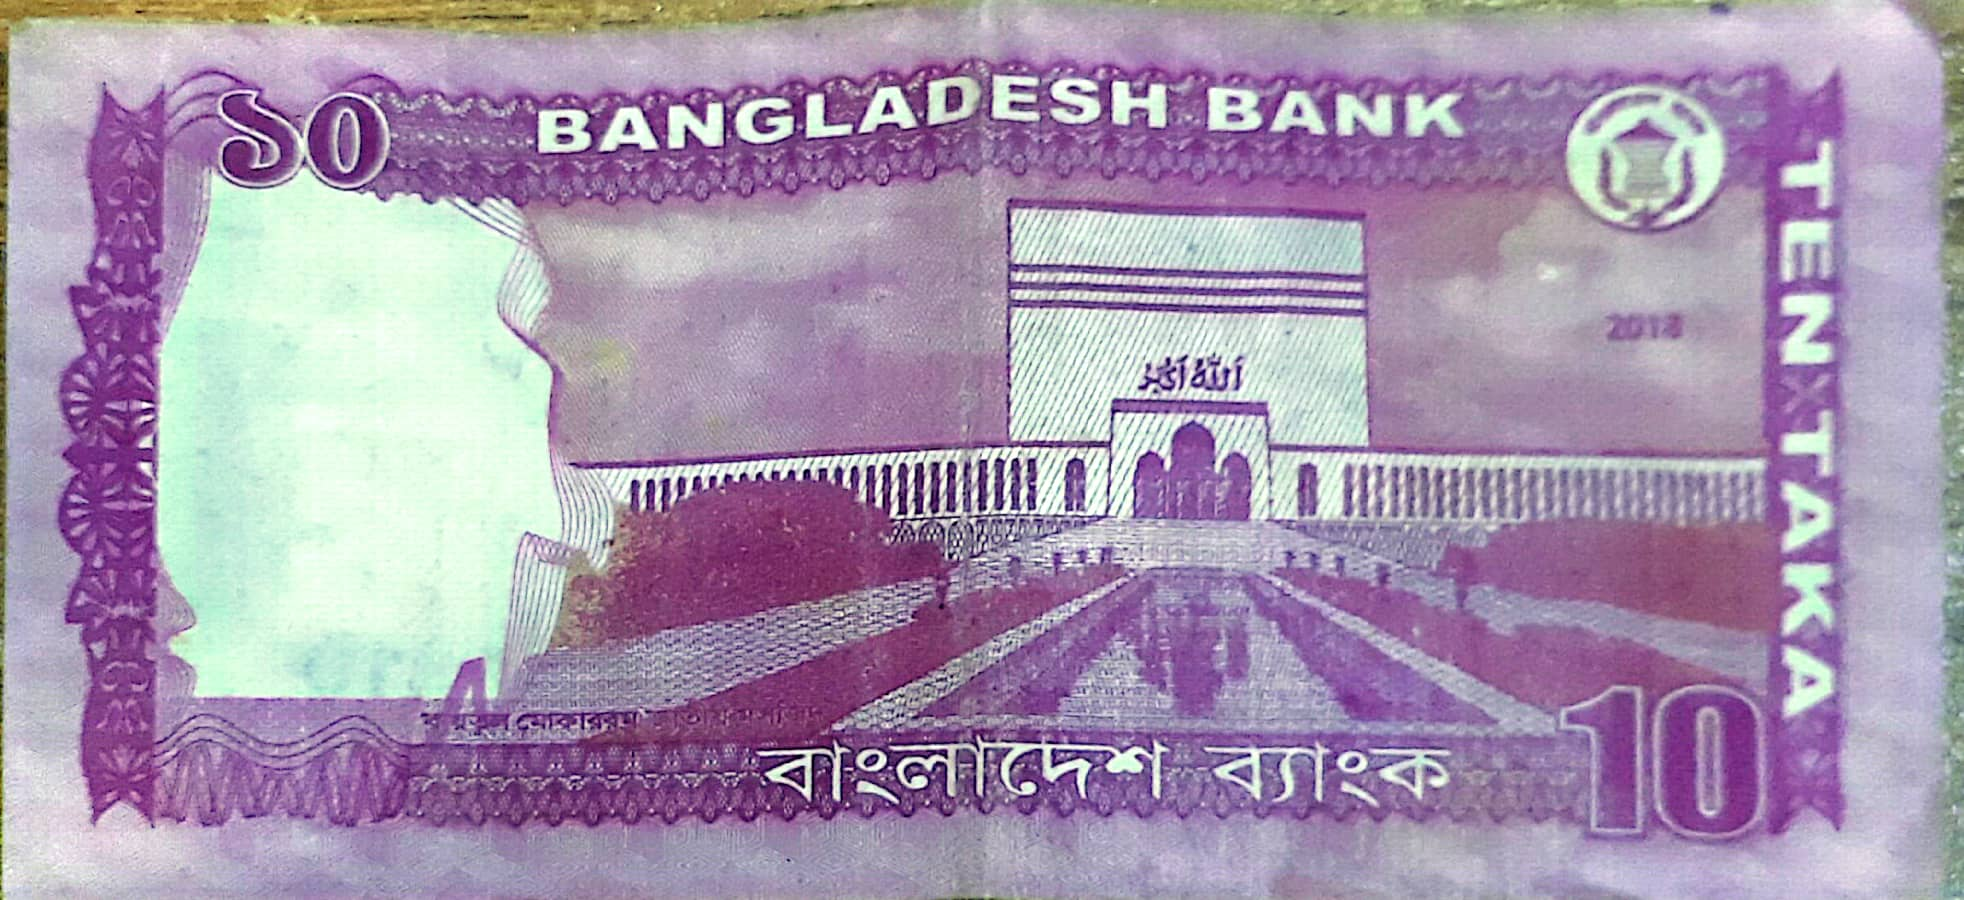
\includegraphics[width=0.45\textwidth]{sample_note_10_taka.jpg}
    \hspace{0.3cm}
    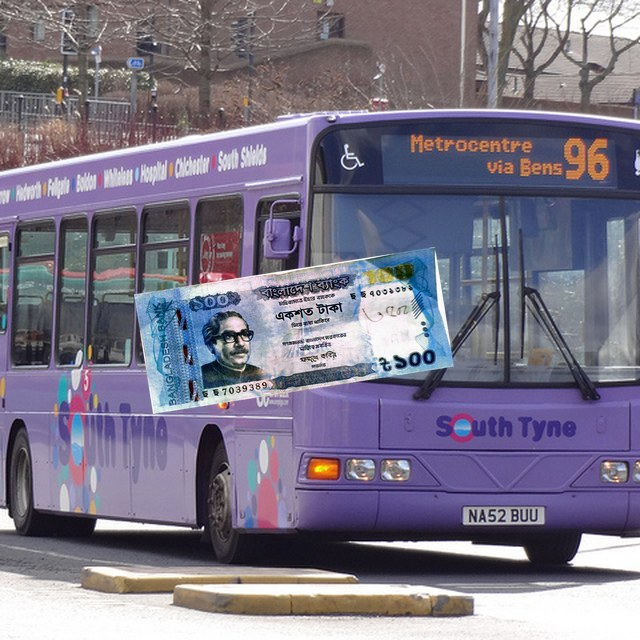
\includegraphics[width=0.45\textwidth]{sample_detection_100_taka.jpg}
    \caption{Left: a 10 Taka note from the local currency dataset. Right: a 100 Taka note placed on a real street background, the kind of cluttered scene the currency detector of Savior Glass is trained to handle.}
    \label{fig:intro_samples}
\end{figure}

This thesis presents \textbf{Savior Glass}, a wearable, offline, Bangla-first smart glass for visually impaired users. Savior Glass is designed around a Raspberry Pi~5 \cite{raspberrypi5}, a camera module mounted near the eyes, five physical push-buttons and an earphone or speaker. It offers three main modes that a user cycles with a single button: \textit{text reading} (Bangla and English OCR), \textit{object detection} (spoken names of everyday objects in Bangla), and \textit{currency detection} (denomination of Bangladeshi Taka notes). On top of these modes, the project developed a multi-view counterfeit-note authenticator, a facial-expression recogniser that makes the spoken feedback emotion-aware, haptic confirmation, and an optional online scene-description mode. All core functions run on the device itself without internet access once the models are installed.

The work is also a data-engineering study. Public Bangladeshi currency datasets consist mainly of clean, close-up scans of notes. A model trained only on them learns that ``the whole frame is the note'' and fails on a live camera. We therefore built a copy-paste compositing pipeline that places notes on real photographs and generates exact bounding boxes automatically. For counterfeit detection we worked with a six-view genuine/counterfeit note dataset and found that a model trained only on six views collapses when it sees one view, which led to a prefix-robust training protocol. Throughout the thesis, every accuracy number is taken from a saved evaluation file, and results that are not yet measured, such as Raspberry Pi~5 latency or a study with visually impaired participants, are stated as not measured.


\section{Problem Statement}
\label{sec:Problem Statement}
Visually impaired people in Bangladesh depend on family members, shopkeepers or passers-by to read text, identify objects and handle money. This dependence creates three concrete risks: loss of independence in daily activities, exposure to fraud when receiving change or counterfeit notes, and loss of privacy when others must read personal documents. Existing assistive technologies do not solve these problems for Bangladeshi users.

Common limitations in current solutions include:

\begin{itemize}[noitemsep]
    \item High cost of commercial smart glasses and dependence on a smartphone or subscription;
    \item Dependence on cloud services for OCR, recognition or speech, which fails without internet;
    \item English-centric design, with little or no support for Bangla text and Bangla speech;
    \item No support for recognising Bangladeshi Taka, and almost no support for detecting counterfeit notes;
    \item Touch-screen or app-based interfaces that are hard to use without sight.
\end{itemize}

On the technical side, two specific problems had to be solved. First, Bangladeshi currency recognition models trained on clean note images do not transfer to real camera frames in which the note is small, rotated, partly lit and surrounded by clutter. Second, counterfeit authentication needs several close views of a note, but a blind user cannot guarantee that all views will be captured; a model that is accurate only when all six views are present is not usable in practice.

This project addresses these gaps and develops Savior Glass, an offline assistive smart glass that uniquely integrates:

\begin{itemize}[noitemsep]
    \item Bangla and English text reading with a capture-then-read interaction;
    \item Everyday object announcement with Bangla labels and repetition control;
    \item Detection of all nine Bangladeshi Taka denominations in cluttered scenes;
    \item Multi-view genuine/counterfeit authentication that stays accurate with fewer views;
    \item Offline Bangla/English speech, haptic feedback and physical buttons for control.
\end{itemize}


\section{Objectives}
\label{sec:Objective}

The primary objective of this project is to design, implement and evaluate Savior Glass, an affordable, offline, Bangla-first assistive smart glass for visually impaired people. The specific goals are:

\begin{enumerate}[noitemsep]
    \item To build a wearable prototype on Raspberry Pi~5 that is operated entirely through physical buttons and audio feedback.
    \item To provide Bangla and English text reading using on-device OCR and offline text-to-speech.
    \item To announce everyday objects in front of the user in Bangla using a real-time object detector.
    \item To detect and name all nine denominations of Bangladeshi Taka in real-world scenes, by creating a large synthetic detection dataset without manual annotation.
    \item To develop a counterfeit-note authenticator that remains reliable when only one or a few views of the note are available.
    \item To add supporting features such as emotion-aware speech, haptic confirmation and a Windows development harness.
    \item To evaluate every module with standard metrics on held-out data and to report the results and gaps honestly.
\end{enumerate}

Ultimately, the objective is to create a human-centred, low-cost and privacy-preserving assistive device that increases the independence of visually impaired people in Bangladesh.

\section{Scope of the Study}
\label{sec:Scope of the Study}

This research is concerned with the design, development and technical evaluation of a camera-based wearable assistant. The main functions of the system are the following:

\begin{itemize}
    \item \textbf{Text Reading (OCR):} Recognition of printed Bangla and English text from the camera image and reading it aloud on request.

    \item \textbf{Object Detection:} Periodic detection of the 80 COCO object classes (person, chair, bottle, bus and so on) and announcement of the most relevant ones in Bangla.

    \item \textbf{Currency Detection:} Localisation and classification of the nine Bangladeshi Taka denominations, spoken in Bangla, with vibration confirmation.

    \item \textbf{Currency Authentication:} Classification of a note as genuine or counterfeit from one to six close-up views.

    \item \textbf{Emotion-Aware Feedback:} Recognition of the facial expression of a person in front of the user, used to adapt the spoken feedback.
\end{itemize}

The study does not cover navigation, obstacle distance measurement, GPS, or voice-command control in Bangla, although parts of these exist as experimental code. Model accuracy is evaluated on public and local datasets on a laptop; latency on the Raspberry Pi~5 itself and a formal study with visually impaired participants are outside what has been measured so far and are presented as future work. The glass is an aid; it does not replace a white cane, a guide or a bank's counterfeit-detection equipment.


\section{Research Questions}
\label{sec:Research Question}

This research addresses the following questions:

\begin{enumerate}
    \item How can a fully offline, multi-function assistive smart glass with Bangla support be designed and implemented on a low-cost embedded platform such as the Raspberry Pi~5?

    \item Can a detector trained on synthetically composited images, generated without any manual annotation, recognise Bangladeshi Taka notes in cluttered real-world scenes?

    \item Why does a multi-view counterfeit authenticator trained on a fixed number of views fail when fewer views are available, and can a training protocol fix this?

    \item How accurately can existing open OCR engines read Bangla and English text for assistive use, and where are their weaknesses?

    \item How can the interaction design (buttons, capture/read separation, cooldowns, Bangla speech) be made suitable for users without sight?
\end{enumerate}

\section{Contributions}
\label{sec:contributions}
The main contributions of this thesis are:
\begin{enumerate}[noitemsep]
    \item A complete, offline, three-mode assistive smart-glass system (Savior Glass) with Bangla-first speech, physical button control, systemd deployment on Raspberry Pi~5 and a Windows test harness.
    \item A copy-paste compositing pipeline that turns 5,073 clean note images and 1,500 COCO backgrounds into a 22,315-image detection dataset with automatic, pixel-exact bounding boxes, and a YOLOv8s Taka detector trained on it.
    \item A prefix-robust multi-view training protocol for counterfeit authentication that removes the train/test mismatch in the number of views and holds accuracy between 97.1\% and 98.1\% from one to six views on a note-disjoint test set.
    \item An honest, file-backed evaluation of every module, including negative results and a list of measurements that are still missing.
\end{enumerate}


\section{Thesis Structure}

This thesis is organized into seven chapters, each addressing a specific aspect of the project. The chapters are outlined as follows:

\begin{itemize}
    \item \textbf{Chapter 1: Introduction} \\
    This chapter provides the background, problem statement, objectives, scope, research questions, contributions and thesis structure.

    \item \textbf{Chapter 2: Literature Review} \\
    This chapter reviews assistive technologies for visually impaired people, smart glasses, OCR and text-to-speech systems, object detection, and Bangladeshi currency recognition.

    \item \textbf{Chapter 3: System Design and Methodology} \\
    This chapter describes the framework, hardware components, software design and the methodology of Savior Glass.

    \item \textbf{Chapter 4: Implementation Process} \\
    This chapter explains how each module was implemented, integrated and deployed.

    \item \textbf{Chapter 5: Dataset and Data Engineering} \\
    This chapter presents the datasets used, the synthetic compositing pipeline and the data splits.

    \item \textbf{Chapter 6: Results and Discussion} \\
    This chapter reports the measured performance of each module, discusses the findings and states the limitations.

    \item \textbf{Chapter 7: Conclusion and Future Work} \\
    This chapter summarises the work, its social impact and the directions for future research.
\end{itemize}


\clearpage
\chapter{Literature Review}
\label{chap:literature}

\section{Assistive Technology for the Visually Impaired}
\label{sec:assistive}

Assistive technology (AT) for blind and visually impaired (BVI) people aims to replace or supplement visual information with another channel, usually sound or touch. Traditional aids such as the white cane, guide dogs and Braille are reliable but provide limited information: a cane detects an obstacle but cannot say what it is, and Braille is available only for a small fraction of printed material. Over the last two decades, the combination of low-cost cameras, embedded processors and deep learning has made it possible to build devices that ``see'' on behalf of the user and describe the scene through speech \cite{at_review2025, wearable_review2024}.

A recent bibliometric review of 533 articles on wearable mobility aids published between 2014 and 2024 shows a clear shift from single-sensor prototypes towards user-centred, multi-function systems that combine computer vision, audio and haptic feedback \cite{wearable_review2024}. Reviews of image-to-voice systems describe a common two-stage pipeline: a vision model converts the image into text or labels, and a text-to-speech (TTS) engine converts that text into audio \cite{imgspeech_review2024}. Savior Glass follows the same general pipeline, but specialises each stage for Bangla and for offline use.

\section{Historical Background and Evolution}
\label{sec:history}

Early reading machines combined a scanner, a hand-crafted OCR engine and concatenative speech synthesis. Assistive reading systems of that period localised text with connected-component labelling and histogram analysis on binarised images and produced speech through recorded phoneme units \cite{assistreading2014, speechiface2013}. These systems worked on clean printed pages but not on natural scenes.

The next generation moved to portable hardware. FingerReader used a finger-worn camera to read printed text on the go \cite{fingerreader2014}, and product-label readers used motion to isolate a held object in front of a Pi camera \cite{labelreading2017}. With the arrival of the Raspberry Pi, many low-cost readers were built from a Pi board, a USB or Pi camera, Tesseract OCR and a speaker \cite{readingaid_rpi2023, visionvoice2024, cameraocr2023, itra2022, imgproc_text2019}. Most of these systems read English only and use Google Text-to-Speech, which requires an internet connection.

In parallel, smart glasses appeared. Student-GLASS built a camera glass with voice requests and auditory feedback on a microcontroller \cite{studentglass2017}. A Google Glass system used Microsoft Azure Custom Vision in the cloud for scene recognition and bone-conduction audio \cite{googleglass2021}. A deep learning smart glass published in \textit{Electronics} combined low-light enhancement, object recognition and salient object detection for night-time assistance \cite{smartglass_mdpi2021}. More recently, AIris placed a camera on eyewear and sent images to a remote server for face recognition, scene description and text reading \cite{airis2024}. The trend is towards richer functions, but also towards heavier dependence on remote computation.

\section{Key Technologies in Smart Assistive Glasses}
\label{sec:keytech}

\subsection{Embedded Computing Platforms}
Raspberry Pi boards dominate low-cost assistive prototypes because they run a full Linux system, support Python, OpenCV and PyTorch, and provide GPIO pins for buttons and motors. Earlier projects used the Raspberry Pi 3 or 4 \cite{readingaid_rpi2023, visionvoice2024, aiblind2025, voicereading2025}. The Raspberry Pi~5 used in this work has a quad-core Cortex-A76 CPU at 2.4~GHz, which is a large step in CPU performance over the Pi 4 \cite{raspberrypi5}. Arduino-based glasses \cite{lightweight_glass2025} are lighter and cheaper but cannot run deep neural networks.

\subsection{Optical Character Recognition}
OCR converts an image of text into machine-readable characters. Tesseract is the most common engine in assistive readers \cite{readingaid_rpi2023, cameraocr2023, itra2022, textreview2022}. It works well on clean, horizontal, printed text but struggles with scene text and non-Latin scripts. Deep learning OCR engines such as EasyOCR combine a CRAFT-style text detector with a recognition network and support more than 80 languages including Bangla \cite{easyocr, easyocr_reader2022}. Cloud OCR, for example Google Cloud Vision \cite{cloudocr2019}, gives higher accuracy but requires internet access and sends the user's images to a third party. Bangla OCR is a harder problem because of the large number of conjunct characters (\textit{juktakkhor}), the connecting head line (\textit{matra}) and vowel diacritics above and below the base letter. Deep learning classifiers such as Inception V3, VGG-16 and Vision Transformers have been applied to isolated handwritten Bangla characters \cite{banglaocr2021}, and datasets such as Ekush provide large, writer-labelled collections of Bangla characters \cite{ekush}.

\subsection{Object Detection}
Object detection locates and labels objects in an image. The YOLO family of single-stage detectors \cite{redmon2016yolo} is the most common choice in assistive devices because it runs in real time \cite{echolight2025, aiblind2025, voicereading2025, ai_nlp2025, ivsmart2024}. YOLOv8 from Ultralytics \cite{ultralytics} is anchor-free, uses a CSPDarknet backbone with C2f blocks, a PAN-FPN neck and a decoupled head, and is provided in nano, small, medium and larger sizes. Pre-trained YOLOv8 models detect the 80 classes of the COCO dataset \cite{coco}.

\subsection{Speech Output and Feedback}
Speech synthesis has progressed from concatenative synthesis to neural TTS \cite{stt_tts2023}. Online engines such as gTTS give natural voices but need the internet. Offline engines include espeak-ng, a compact formant synthesiser that supports Bangla \cite{espeakng}, and Piper, a fast local neural TTS system that runs on a Raspberry Pi \cite{piper}. Bone-conduction headsets and vibration motors are used as additional channels so that the user can still hear the environment \cite{googleglass2021, lightweight_glass2025}.

\section{Currency Recognition and Authentication}
\label{sec:currency_lit}

Currency recognition is an important task for visually impaired people because banknotes of different values often have similar size and texture. Classical systems identify the country and denomination with template matching, colour analysis in the LAB space and size measurements \cite{currency2017, currency2023}. For Bangladeshi Taka, an early neural network with axis-symmetrical masks reported 98.57\% average accuracy over eight denominations \cite{axissym}, lightweight CNNs have been used for real-time recognition for visually impaired users \cite{cnnrealtime}, and a dual-stream MobileNet/EfficientNet model has been proposed for robust recognition \cite{dualstream}. These methods are whole-image classifiers: they assume that one note fills the image.

Detection-based approaches localise the note in a full scene. The NSTU-BDTAKA dataset provides 3,111 manually annotated images for Taka detection with YOLOv5, reaching a precision of 0.95 and a recall of 0.93 \cite{nstubdtaka2024}. A YOLOv8-nano model with a squeeze-and-excitation head for US Dollar, Euro and Taka detection reported 0.972 mAP@0.5 and 0.804 mAP@0.5:0.95 \cite{yolov8nse}. Domain randomisation with synthetic images has been shown to transfer to real object detection \cite{domainrand}, which motivates the compositing approach used in this thesis. Among assistive applications, BLIND ASSIST \cite{blindassist2021}, Divya-Drishti \cite{divyadrishti2021} and VisioGuide \cite{visioguide2025} include a currency feature, usually for Indian Rupees and usually on a smartphone.

Counterfeit detection is much less studied in assistive systems. Bank equipment uses ultraviolet light, magnetic ink and infrared sensors, which are not available on a glass. With a visible-light camera, the security thread, hologram strip, watermark and micro-printing must be inspected from close views, and one view is often not enough. This motivates the multi-view authenticator in this work.

\section{Real-World Applications}
\label{sec:applications}

\subsection{Reading Assistants}
Reading assistants are the most common category. Raspberry Pi readers with Tesseract and gTTS \cite{readingaid_rpi2023, visionvoice2024, cameraocr2023}, translators from English to regional languages \cite{readingaid_rpi2023}, and deep learning readers that also describe images in printed documents \cite{dlreader2022} have been reported. Sinhala and Kannada readers \cite{visioguide2025} show that local-language support is a real need in South Asia.

\subsection{Multi-Function Wearables}
Multi-function devices combine several modules. The Third Eye clips a camera to spectacles and uses a smartphone for text, face and object recognition \cite{thirdeye2019}. A Raspberry Pi~4 system with LiDAR and Camera Module~3 combines YOLOv8n detection, Tesseract OCR, face detection and distance measurement \cite{aiblind2025}. Other systems add ultrasonic obstacle sensing, GPS and GSM alerts \cite{navassist2024, smartglass_vip2025, obstacle_rpi2020}. EchoLight uses YOLOv5, OCR and TTS through a bone-conduction headset \cite{echolight2025}.

\subsection{Mobile Applications}
Smartphone apps such as BLIND ASSIST \cite{blindassist2021}, IV Smart \cite{ivsmart2024} and assistants based on NLP \cite{ai_nlp2025} are convenient but require the user to aim a phone and use a touch screen, which many blind users find difficult.

\section{Comparative Evaluation of Assistive Vision Systems}
\label{sec:comparison}

Table~\ref{tab:assistive_compare} compares representative systems from the literature with the system developed in this work. The comparison shows that most systems have strong individual capabilities; however, few combine offline operation, local-language support and local currency handling in one wearable design.

\begin{table}[!htbp]
\centering
\caption{Overview of assistive vision systems for visually impaired users, with key technologies, strengths and limitations}
\label{tab:assistive_compare}
\begin{tabular}{|p{1.4cm}|p{2.4cm}|p{3.6cm}|p{3.3cm}|p{3.3cm}|}
\hline
\textbf{Citation} & \textbf{System} & \textbf{Key Technologies} & \textbf{Strengths} & \textbf{Limitations} \\ \hline
\cite{smartglass_mdpi2021} & Deep learning smart glass & Low-light enhancement CNN, transformer object recognition & Works at night, rich scene information & Heavy models, English labels, no currency \\ \hline
\cite{googleglass2021} & Google Glass scene analysis & Azure Custom Vision (cloud), bone conduction & Commercial glass hardware, real-time & Needs internet, expensive glass \\ \hline
\cite{airis2024} & AIris & Eyewear camera, Raspberry Pi, remote server & Face, text, scene description & Remote processing, English \\ \hline
\cite{aiblind2025} & RPi 4 blind assistance & YOLOv8n, Tesseract, LiDAR, Haar faces & Distance measurement, several modules & English OCR only, no currency \\ \hline
\cite{visionvoice2024} & Vision Voice & Raspberry Pi 3, PyTesseract, gTTS & Low cost, simple & Text only, online TTS \\ \hline
\cite{blindassist2021} & BLIND ASSIST & Android, TensorFlow Lite currency, OCR & One app, currency feature & Phone and touch screen needed \\ \hline
\cite{nstubdtaka2024} & NSTU-BDTAKA & YOLOv5, 3,111 labelled images & Bangladeshi Taka detection & Manual labels, no assistive device \\ \hline
\textbf{This work} & \textbf{Savior Glass} & \textbf{EasyOCR bn/en, YOLOv8, synthetic Taka data, multi-view authenticator, Piper/espeak-ng} & \textbf{Offline, Bangla speech, 9 Taka classes, counterfeit check, buttons} & \textbf{Pi~5 latency and user study not yet measured} \\ \hline
\end{tabular}
\end{table}
\FloatBarrier

Table~\ref{tab:currency_compare} focuses on currency recognition. Direct numerical comparison should be read with care because each study uses a different dataset, class set and test protocol.

\begin{table}[!htbp]
\centering
\caption{Comparison of currency recognition methods related to Bangladeshi Taka}
\label{tab:currency_compare}
\begin{tabular}{|p{3.6cm}|p{1.8cm}|p{2.2cm}|p{1.6cm}|p{1.6cm}|p{2.4cm}|}
\hline
\textbf{Work} & \textbf{Task} & \textbf{Labels} & \textbf{mAP@0.5} & \textbf{mAP@ 0.5:0.95} & \textbf{P / R or Acc.} \\ \hline
Axis-symmetrical masks \cite{axissym} & Classify & Image-level & -- & -- & 98.6\% acc. \\ \hline
YOLOv5 Taka \cite{nstubdtaka2024} & Detect & 3,111 manual & -- & -- & 0.95 / 0.93 \\ \hline
YOLOv8n-SE \cite{yolov8nse} & Detect (multi-currency) & Manual & 0.972 & 0.804 & 0.965 / 0.952 \\ \hline
\textbf{This work (YOLOv8s)} & \textbf{Detect (9 BDT)} & \textbf{22,315 automatic} & \textbf{0.995*} & \textbf{0.847*} & \textbf{0.998 / 0.997*} \\ \hline
\end{tabular}

\vspace{2pt}
{\footnotesize *Measured on held-out synthetic composites; see Chapter~\ref{chap:results} for the evaluation on raw phone photographs.}
\end{table}
\FloatBarrier

\section{Key Research Areas Relevant to Savior Glass}

Recent work relevant to this thesis falls into four areas, summarised in Table~\ref{tab:key_areas}.

\textbf{Text Reading Systems} use OCR and TTS to read printed material. They are mature for English but weak for Bangla and depend on online speech.

\textbf{Smart Glasses and Wearables} integrate cameras, processors and audio on the body. They increasingly rely on cloud processing for advanced functions.

\textbf{Object and Scene Recognition} relies on YOLO-family detectors and captioning models, usually with English labels.

\textbf{Currency Recognition and Authentication} covers denomination classification and detection; authentication with a visible-light camera is still largely unexplored in assistive devices.

\begin{table}[!htbp]
\centering
\begin{tabular}{|p{4cm}|p{10.5cm}|}
\hline
\textbf{Citation(s)} & \textbf{Category and Function/Details} \\
\hline
\cite{fingerreader2014,assistreading2014,readingaid_rpi2023,visionvoice2024,cameraocr2023,itra2022,dlreader2022} &
\textbf{Text Reading Systems:} Finger-worn and Raspberry Pi readers, Tesseract and EasyOCR engines, image description in printed documents, translation to regional languages. \\
\hline
\cite{studentglass2017,smartglass_mdpi2021,googleglass2021,airis2024,thirdeye2019,lightweight_glass2025,smartglass_vip2025} &
\textbf{Smart Glasses and Wearables:} Camera glasses with voice feedback, cloud scene analysis, lightweight Arduino glasses with vibration, IoT emergency glasses. \\
\hline
\cite{echolight2025,aiblind2025,voicereading2025,ivsmart2024,navassist2024,ai_nlp2025} &
\textbf{Object and Scene Recognition:} YOLOv4/v5/v8 object detection, LiDAR and ultrasonic distance, face detection, navigation with GPS. \\
\hline
\cite{currency2017,currency2023,axissym,nstubdtaka2024,yolov8nse,blindassist2021,divyadrishti2021} &
\textbf{Currency Recognition:} Template and colour matching, neural classifiers, YOLO detection of Taka and other currencies, currency features in mobile apps. \\
\hline
\end{tabular}
\caption{Key research categories in assistive vision technology}
\label{tab:key_areas}
\end{table}
\FloatBarrier

\section{Research Gap}
\label{sec:gap}
From the review, the following gaps are identified:
\begin{enumerate}[noitemsep]
    \item Very few assistive glasses work completely offline; most depend on cloud OCR, cloud recognition or online TTS.
    \item Bangla is rarely supported, either for reading text or for speaking results.
    \item Bangladeshi Taka detection has been studied as a stand-alone computer vision task, but it has not been integrated in a wearable, and detectors rely on small, manually labelled datasets.
    \item Counterfeit-note checking with a normal camera has not been addressed in assistive devices, and the problem of an unreliable number of captured views has not been studied.
    \item Many prototypes are reported without quantitative evaluation of each module.
\end{enumerate}
Savior Glass is designed to address these gaps.

\clearpage
\chapter{System Design and Methodology}
\label{chap:design}

\section{Framework of Savior Glass}
\label{sec:framework}

The framework of Savior Glass follows an input--process--output structure (Figure~\ref{fig:framework}). The user gives commands only through physical buttons, the camera provides the visual input, the on-board models interpret the scene according to the active mode, and the result is returned through speech and vibration.

\subsection*{Input}
\begin{itemize}[noitemsep]
    \item \textbf{Camera frames:} 640$\times$480 colour frames from a Raspberry Pi Camera Module~2 (Sony IMX219, fixed focus) read through the Picamera2 library \cite{picamera2}, or from a USB webcam.
    \item \textbf{Button events:} five push-buttons for MODE, ACTION, READ, VOLUME~UP and VOLUME~DOWN, read through GPIO interrupts.
\end{itemize}

\subsection*{Process}
\begin{itemize}[noitemsep]
    \item \textbf{Mode manager:} keeps the active mode (text, object, currency, online description, emotion) and routes frames and button events to it.
    \item \textbf{Vision models:} EasyOCR for Bangla/English text, YOLOv8 for COCO objects, a YOLOv8s Taka detector, a multi-view authenticator and a watermark classifier for genuine/counterfeit notes, and an EfficientNet-V2-S expression recogniser.
    \item \textbf{Language processing:} Bangla script detection, mixed-script segmentation and translation of labels to Bangla.
\end{itemize}

\subsection*{Output}
\begin{itemize}[noitemsep]
    \item \textbf{Speech:} Piper neural TTS or espeak-ng through the ALSA audio system, in Bangla or English.
    \item \textbf{Vibration:} a short pulse from a vibration motor that confirms a detected note.
    \item \textbf{Field log:} one line per event (button, mode, result, time taken) and periodic system readings in two CSV files.
\end{itemize}

\begin{figure}[htbp]
\centering
\begin{adjustbox}{max width=\textwidth}
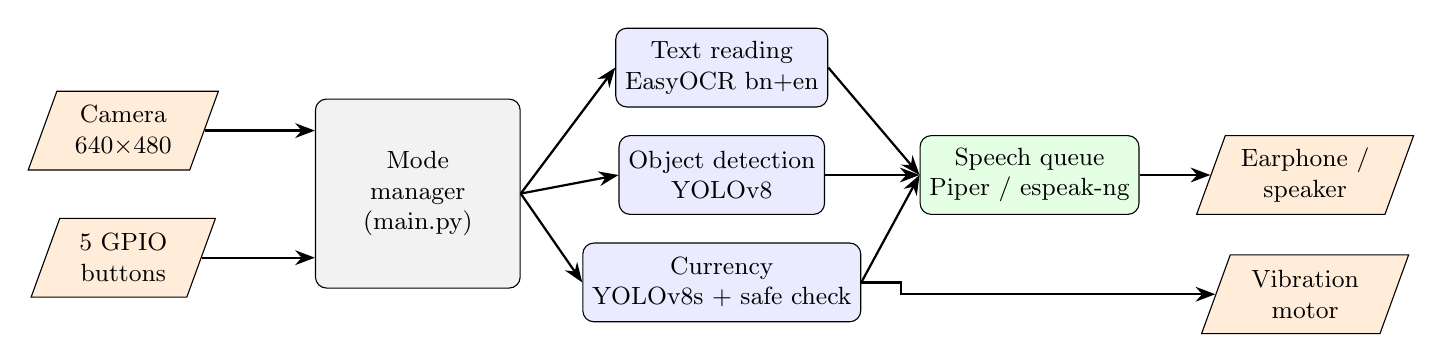
\begin{tikzpicture}[node distance=0.6cm and 1.0cm]
  \node[io] (cam) {Camera\\640$\times$480};
  \node[io, below=of cam] (btn) {5 GPIO\\buttons};
  \node[block, right=1.4cm of cam, yshift=-0.8cm, minimum height=2.4cm, fill=gray!10] (mgr) {Mode\\manager\\(main.py)};
  \node[block, right=1.2cm of mgr, yshift=1.6cm] (ocr) {Text reading\\EasyOCR bn+en};
  \node[block, below=0.35cm of ocr] (obj) {Object detection\\YOLOv8};
  \node[block, below=0.35cm of obj] (cur) {Currency\\YOLOv8s + safe check};
  \node[block, right=1.2cm of obj, fill=green!10] (tts) {Speech queue\\Piper / espeak-ng};
  \node[io, right=0.9cm of tts] (out) {Earphone /\\speaker};
  \node[io, below=0.5cm of out] (hap) {Vibration\\motor};
  \draw[arrow] (cam.east) -- (mgr.west |- cam.east);
  \draw[arrow] (btn.east) -- (mgr.west |- btn.east);
  \draw[arrow] (mgr.east) -- (ocr.west);
  \draw[arrow] (mgr.east) -- (obj.west);
  \draw[arrow] (mgr.east) -- (cur.west);
  \draw[arrow] (ocr.east) -- (tts.west);
  \draw[arrow] (obj.east) -- (tts.west);
  \draw[arrow] (cur.east) -- (tts.west);
  \draw[arrow] (tts.east) -- (out.west);
  \draw[arrow] (cur.east) -- ++(0.5,0) |- (hap.west);
\end{tikzpicture}
\end{adjustbox}
\caption{Input--process--output framework of Savior Glass. The emotion mode and the optional online mode use the same path and are omitted for clarity.}
\label{fig:framework}
\end{figure}


\section{Overview of Savior Glass System Design}
\label{sec:overview}

Savior Glass is designed as a pair of spectacles with a small camera at the bridge and a processing unit worn at the waist or in a pocket. The design follows five principles derived from the problems described in Chapter~\ref{chap:introduction}:

\begin{enumerate}[noitemsep]
    \item \textbf{Offline first:} every core function runs locally. The only online feature is an optional scene-description mode that the user must choose on purpose.
    \item \textbf{Bangla first:} mode names, object names and currency names are spoken in Bangla; text is read in the language in which it is written.
    \item \textbf{Buttons, not screens:} the device has no display. Every function is reachable with five buttons that can be found by touch.
    \item \textbf{On-demand heavy work:} slow tasks (OCR, currency) run only when the user presses ACTION; only the object mode scans continuously.
    \item \textbf{Safe before decisive:} when the device is not sure, it says so. It never tells the user that a note is counterfeit.
\end{enumerate}

\subsection{General Overview of Savior Glass}
When the device boots it announces that the smart glass is starting and then speaks the name of the active mode. The user cycles through the modes with the MODE button. In \textit{text reading mode}, ACTION captures and recognises text, speaks it once and stores it, and READ speaks the stored text again. In \textit{object mode}, the glass scans the scene every 1.5~seconds and announces up to three objects, for example ``in front: chair, person''. In \textit{currency mode}, ACTION detects the note, speaks its value in Bangla and gives a vibration pattern; for a 500 or 1,000 Taka note it then gives the result of the safe check, and it can ask the user to hold the note up to a light for the watermark check. In \textit{emotion mode}, ACTION announces the facial expression of the nearest face. The \textit{online mode} describes the scene when the internet and an API key are available. VOLUME~UP and VOLUME~DOWN change the volume in 10\% steps. The name of a mode is spoken immediately after MODE is pressed, while its model loads in the background.

\subsection{Structural Characteristics of Savior Glass}
The prototype consists of a spectacle frame carrying the camera module, a cable to the Raspberry Pi~5 in a small enclosure, a push-button pad, a vibration motor and an earphone. Separating the processing unit from the frame keeps the glasses light and moves the heat of the processor away from the face.

\subsection{Interactive Features and Interface Design}
Several interaction decisions were made specifically for users without sight:
\begin{itemize}[noitemsep]
    \item \textbf{Capture is separated from reading.} The user holds the camera still while pressing ACTION, and can then relax and listen by pressing READ. The text can be replayed as often as needed.
    \item \textbf{Repetition control.} In object mode, each object class has a 4-second cooldown so the glass does not repeat ``chair, chair, chair''.
    \item \textbf{Speech interruption.} Switching mode clears the speech queue immediately so the user does not wait for old messages.
    \item \textbf{Mixed-script speech.} A sentence such as ``Bus 96 Metrocentre'' inside Bangla text is split, and each part is sent to the correct voice.
    \item \textbf{Vibration confirmation.} A vibration confirms that a note was detected, even in a noisy market.
    \item \textbf{Guided capture.} For the watermark check the glass tells the user what is wrong with the picture (``too dark'', ``hold still'') instead of silently failing.
    \item \textbf{Cautious wording.} The counterfeit check has two spoken outcomes, ``likely genuine'' and ``check by hand''. The word ``counterfeit'' is never spoken.
\end{itemize}


\section{Hardware Components}
\label{sec:hardware}

Table~\ref{tab:hardware} summarises the hardware of the prototype. Each component is described below.

\begin{table}[!htbp]
\centering
\caption{Hardware components of Savior Glass}
\label{tab:hardware}
\begin{tabular}{|p{3.3cm}|p{5.4cm}|p{5.3cm}|}
\hline
\textbf{Component} & \textbf{Specification} & \textbf{Role} \\ \hline
Raspberry Pi~5 & Quad-core Cortex-A76, 2.4 GHz, 4/8 GB RAM & Runs all models and the application \\ \hline
Camera Module 2 & Sony IMX219 sensor, fixed focus, used at 640$\times$480 & Captures the scene \\ \hline
Push-buttons (5) & Momentary, wired to GND, BCM 17/27/24/22/23 & MODE, ACTION, READ, VOL+, VOL$-$ \\ \hline
Vibration motor & Driven by PWM on BCM 13 & Haptic feedback \\ \hline
Earphone / speaker & 3.5 mm or USB audio through ALSA & Speech output \\ \hline
Power bank & USB-C power bank (the official Pi~5 supply is rated 5 V, 5 A) & Portable power \\ \hline
Spectacle frame & Frame with camera mount at the bridge & Wearable form factor \\ \hline
\end{tabular}
\end{table}

\subsection*{Processing Unit}
The Raspberry Pi~5 is the brain of the system. It runs Raspberry Pi OS (64-bit), Python~3, OpenCV, PyTorch and ONNX Runtime. All inference runs on the CPU. The board also provides the GPIO pins for the buttons and the vibration motor, and the audio output.

\subsection*{Camera}
The Camera Module~2 (IMX219) is connected through the CSI ribbon cable and read with the Picamera2 library; the OpenCV video interface receives no frames from this camera on the Raspberry Pi~5. A USB webcam can be used instead: the camera manager tries Picamera2 first, then OpenCV, and the choice can be forced with one configuration value. The resolution of 640$\times$480 was chosen as a balance between detail and processing load. The lens has a fixed focus, so close text and notes are not sharp at every distance. The first field test (Section~\ref{sec:field_test}) suggests that this resolution and lens may be too weak for reading; the resolution can be raised with a configuration value.

\subsection*{Buttons}
Five push-buttons connect GPIO pins to ground with internal pull-up resistors. A 250~ms software debounce removes false double presses. The button map is given in Table~\ref{tab:buttons}.

\begin{table}[!htbp]
\centering
\caption{Button map of Savior Glass}
\label{tab:buttons}
\begin{tabular}{|c|c|p{9cm}|}
\hline
\textbf{BCM pin} & \textbf{Button} & \textbf{Behaviour} \\ \hline
17 & MODE & Cycle text $\rightarrow$ object $\rightarrow$ currency $\rightarrow$ online $\rightarrow$ emotion \\ \hline
27 & ACTION & Capture text / force object announcement / detect currency / describe scene / name expression \\ \hline
24 & READ & Speak the stored text \\ \hline
22 & VOL\_UP & Increase volume by 10\% \\ \hline
23 & VOL\_DOWN & Decrease volume by 10\% \\ \hline
\end{tabular}
\end{table}

\subsection*{Audio Output}
Audio is played with the ALSA tools \texttt{aplay} and \texttt{amixer}. The default volume is 80\%. An earphone keeps the information private; a small speaker can be used at home.

\subsection*{Vibration Motor}
A small vibration motor, driven from a PWM pin (BCM 13), gives one short pulse (50~ms) when a note is detected. Separate patterns for a genuine and a counterfeit verdict exist in the code but are not used under the safe policy of Section~\ref{sec:safe_policy}. The motor driver was tested with simulated GPIO on the laptop.

\subsection*{Power}
The system is powered by a USB-C power bank. Battery life has not been measured, because the Raspberry Pi~5 has no battery gauge and a USB-C power meter was not available; it is part of future work.


\section{Software Design}
\label{sec:software}

The software is written in Python and organised as a small core with plug-in modes (Table~\ref{tab:modules}). Every mode implements the same interface (\texttt{activate}, \texttt{deactivate}, \texttt{process\_frame}, \texttt{cleanup}), which allows modes to be added without changing the core.

\begin{table}[!htbp]
\centering
\caption{Software modules of Savior Glass}
\label{tab:modules}
\begin{tabular}{|p{4.2cm}|p{9.8cm}|}
\hline
\textbf{Module} & \textbf{Responsibility} \\ \hline
\texttt{main.py} (SmartGlass) & Life cycle, mode cycling, button routing, object-detection loop, signal handling \\ \hline
\texttt{config.py} & GPIO pins, camera settings, model paths, thresholds, TTS and logging settings \\ \hline
\texttt{button\_handler.py} & GPIO interrupts with debounce \\ \hline
\texttt{utils.py} & Logging, language detection and splitting, TTSEngine, CameraManager \\ \hline
\texttt{modes/ocr\_mode.py} & Bangla/English OCR with store-and-read \\ \hline
\texttt{modes/object\_mode.py} & YOLOv8 object detection, cooldown, Bangla labels \\ \hline
\texttt{ocr\_text\_region.py} & Main text block, line ordering and clean-up rules of the OCR pipeline \\ \hline
\texttt{modes/currency\_mode.py} & YOLOv8s Taka detection, announcement threshold, safe counterfeit check, haptics \\ \hline
\texttt{modes/watermark\_check.py} & Watermark window (learned localizer, SIFT fall-back) and watermark classifier \\ \hline
\texttt{modes/capture\_guide.py} & Brightness and sharpness test of back-lit frames, spoken prompts, study log \\ \hline
\texttt{modes/emotion\_mode.py} & Facial expression of the nearest face \\ \hline
\texttt{modes/claude\_mode.py} & Optional online scene description (internet and API key required) \\ \hline
\texttt{field\_log.py} & Event and system log in CSV, written by a background thread \\ \hline
\texttt{preview.py}, \texttt{live\_diag.py} & Test window with keyboard keys and a live panel of all model outputs \\ \hline
\texttt{voice\_study.py} & Voice-driven questionnaire for the user study \\ \hline
\texttt{roboeye/} package & Authenticator, emotion recogniser, haptics, speaker, Grad-CAM overlay \\ \hline
\texttt{scripts/deploy\_pi5.sh}, \texttt{smart\_glass.service} & Installation on the Pi and start at boot \\ \hline
\end{tabular}
\end{table}

\subsection{Text Reading Module}
\label{sec:ocr_method}
The text module uses EasyOCR \cite{easyocr}: a CRAFT text detector \cite{craft} and a CRNN recogniser with CTC decoding \cite{crnn, ctc}, with the Bangla and English recognisers loaded together. The pipeline used in the glass (called \textit{v2} in the code) was fixed by the experiments of Section~\ref{sec:ocr_results} and has five steps:
\begin{enumerate}[noitemsep]
    \item \textbf{Pre-processing.} The frame is converted to grey scale and its contrast is enhanced with CLAHE \cite{clahe}. Binarisation is not used; it increased the error rate.
    \item \textbf{Detection and recognition.} EasyOCR reads the whole frame once, with detector settings chosen on validation data (text threshold 0.8, low-text threshold 0.3, link threshold 0.4, beam-search decoding).
    \item \textbf{Confidence filter.} Boxes with a confidence below 0.2 are dropped.
    \item \textbf{Main text block.} Starting from the most confident tall box, boxes of similar height that touch it are added. This block is the sign or label the user faces; stray text in the background is dropped.
    \item \textbf{Line ordering and clean-up.} The boxes are grouped into lines and read from top to bottom and left to right. The text is normalised to Unicode NFC, invisible characters and stray symbols at word edges are removed, and digits are put in the script of the words around them.
\end{enumerate}
The main-text-block step reuses the boxes that EasyOCR already returns, so it costs no extra time. If EasyOCR cannot be loaded, the mode falls back to Tesseract~5 \cite{tesseract}, and for single handwritten letters to a small CNN trained on Ekush \cite{ekush}.

\subsection{Object Detection Module}
The object module runs a COCO-pretrained YOLOv8 model (small variant, with the nano variant as fall-back; the nano variant was the one timed on the Raspberry Pi~5) on a 320$\times$240 copy of the frame every 1.5 seconds with a confidence threshold of 0.50. The three most confident unique classes are translated to Bangla with a lookup table of the 80 COCO classes and announced, subject to a per-class cooldown of 4 seconds.

\subsection{Currency Detection Module}
The currency module is a cascade that degrades gracefully when models are missing:
\begin{enumerate}[noitemsep]
    \item \textbf{Stage 0 -- YOLOv8s Taka detector:} the detector trained in this work (Chapter~\ref{chap:dataset}) localises and classifies the nine denominations. On the Raspberry Pi~5 the INT8 ONNX export is used; on a laptop the PyTorch weights. A denomination is announced only when the detector's confidence is at least 0.60. This value was chosen on validation data so that notes of an unknown class, such as the 1 Taka note, are named less often.
    \item \textbf{Stage 1 -- HSV colour profile:} if no detector is available, the largest note-like contour (aspect ratio 1.5--2.8, area $\geq$ 8,000 pixels) is found and its colour histogram is compared with the dominant colour of each denomination.
    \item \textbf{Stage 2 -- MobileNetV3-Small classifier:} if trained weights exist, the note crop is classified and the result overrides Stage~1 when its softmax score is at least 0.65.
\end{enumerate}

\begin{figure}[H]
    \centering
    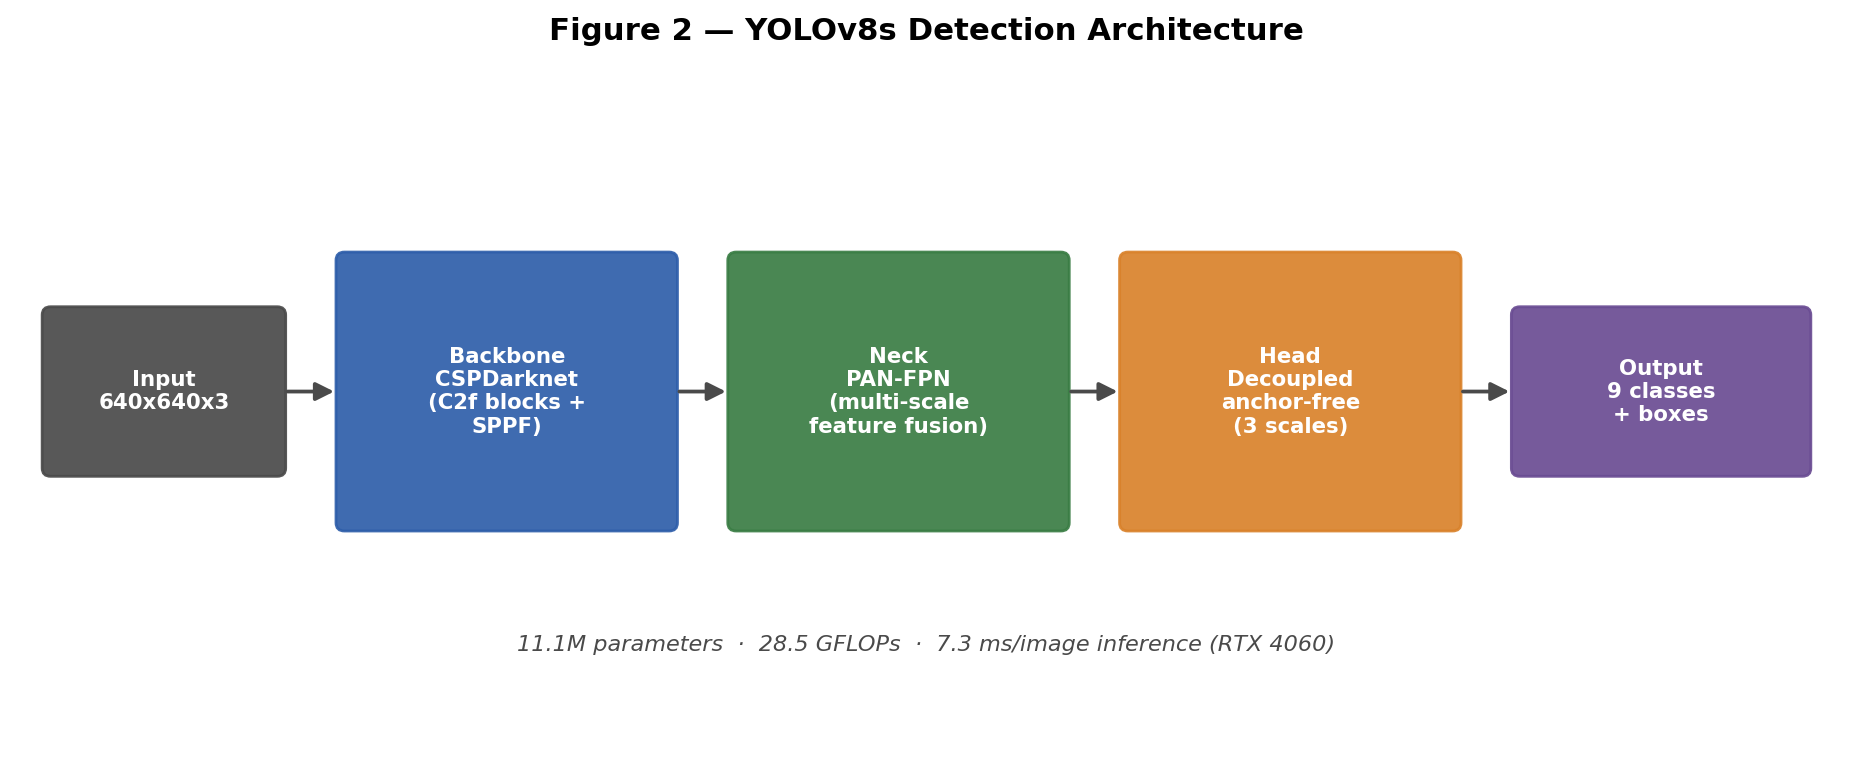
\includegraphics[width=0.9\textwidth]{fig_architecture.png}
    \caption{YOLOv8s detection architecture used for Taka detection: CSPDarknet backbone, PAN-FPN neck and decoupled anchor-free head predicting 9 classes and box coordinates}
    \label{fig:yolo_arch}
\end{figure}

\subsection{Currency Authentication Module}
The authenticator decides whether a note is genuine or counterfeit from up to six close-up views (for example the portrait, the security thread, the hologram strip and the serial number). Each view is resized to 128$\times$128 pixels, normalised, and encoded by a frozen MobileNetV3-Small \cite{mobilenetv3} feature extractor followed by a TinyViT \cite{tinyvit} block. The per-view features are fused by a quality-, diversity-, uncertainty- and information-gain-aware fusion head (called Q-DUIG in this project), which weights sharp, informative and non-redundant views more strongly. The fused feature produces one authenticity logit, whose sigmoid gives the probability $p$ that the note is genuine. In the experiments $p$ is thresholded at 0.5 (Figure~\ref{fig:auth_arch}); the glass uses the stricter policy of Section~\ref{sec:safe_policy}.

\begin{figure}[H]
\centering
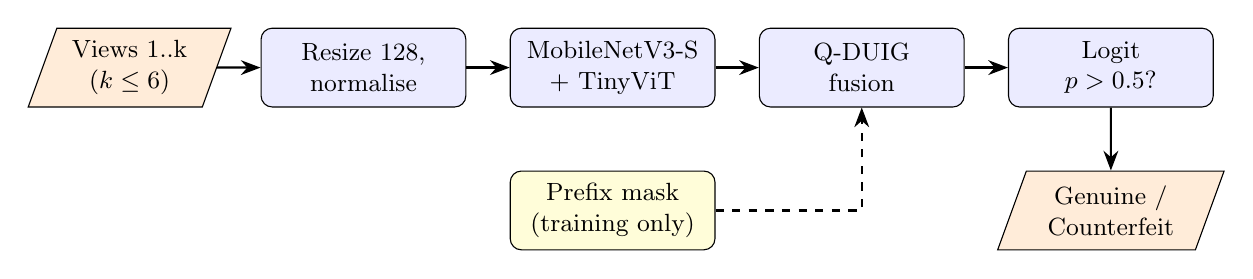
\begin{tikzpicture}[node distance=0.45cm and 0.55cm]
  \node[io] (v) {Views 1..k\\($k\le 6$)};
  \node[block, right=of v] (pre) {Resize 128,\\normalise};
  \node[block, right=of pre] (enc) {MobileNetV3-S\\+ TinyViT};
  \node[block, right=of enc] (fuse) {Q-DUIG\\fusion};
  \node[block, right=of fuse] (head) {Logit\\$p>0.5$?};
  \node[io, below=0.8cm of head] (out) {Genuine /\\Counterfeit};
  \node[block, below=0.8cm of enc, fill=yellow!15] (mask) {Prefix mask\\(training only)};
  \draw[arrow] (v) -- (pre);
  \draw[arrow] (pre) -- (enc);
  \draw[arrow] (enc) -- (fuse);
  \draw[arrow] (fuse) -- (head);
  \draw[arrow] (head) -- (out);
  \draw[arrow, dashed] (mask) -| (fuse);
\end{tikzpicture}
\caption{Multi-view currency authenticator. During prefix-robust training, a random prefix of 1 to 6 views is kept so the model learns to decide with any number of views.}
\label{fig:auth_arch}
\end{figure}

\subsection{Safe Verdict Policy on the Glass}
\label{sec:safe_policy}
The authenticator was trained on close-up views, but the glass sees a whole note. To give the model an input of the shape it knows, the note box found by the Taka detector is resized to 640 pixels in width and turned to landscape, and four windows are cut from it at the positions where JaalTaka views 1 to 4 lie on a note. The positions were measured on 200 training notes by registering each view to a whole-note template with SIFT features \cite{sift} and RANSAC \cite{ransac}. The four windows are scored by the authenticator, which returns $p$.

The spoken verdict follows a rule fixed before any test score was read (called policy~E in the project):
\begin{itemize}[noitemsep]
    \item if $p > \tau$, the glass says \textit{shombhoboto ashol} (``likely genuine'');
    \item otherwise it says \textit{ashol kina hate jachai korun} (``check by hand whether it is genuine'');
    \item it never says \textit{jaal} (``counterfeit'').
\end{itemize}
The threshold $\tau = 0.99959$ is the highest $p$ that any counterfeit note of the validation split received. This is selective prediction \cite{chow1970, selective2017} with a guarantee from conformal prediction \cite{vovk2005}: if a new counterfeit is exchangeable with the $n$ validation counterfeits, the probability that its score is above all of theirs, and so above $\tau$, is
\begin{equation}
P(p_{\text{new}} > \tau) = \frac{1}{n+1},
\end{equation}
which is $1/89 = 1.1\%$ for $n = 88$. The guarantee holds only for notes that resemble the validation notes; a change of camera or of counterfeit print weakens it by at most the total-variation distance between the two distributions. The policy applies to 500 and 1,000 Taka notes, the only denominations in JaalTaka; for other notes the glass says that the check was not done. An image-quality gate rejects dark, blurred or covered frames before any verdict is given.

\subsection{Watermark Check with Guided Capture}
\label{sec:watermark_method}
A genuine note has a watermark that becomes visible when the note is held against a light. The sixth JaalTaka view is such a back-lit photograph. The watermark check has three parts (Figure~\ref{fig:wm_flow}).

\textbf{Capture guide.} After the denomination is spoken, the glass asks the user to hold the note up to a light. Every frame is tested for brightness (mean grey level at least 73.9) and sharpness (variance of the Laplacian at least 106.7, a standard focus measure \cite{pechpacheco2000}). The two limits are the 2nd percentile of the validation back-lit photographs, so about 96\% of acceptable photographs pass. A rejected frame produces a spoken reason, at most every 2.5~seconds, and the guide gives up after 10~seconds.

\textbf{Watermark window.} The first version registered the photograph to a note template with SIFT and RANSAC and cut a fixed box. The current version is a MobileNetV3-Small \cite{mobilenetv3} that regresses the four corners of the window directly from a 320$\times$320 copy of the photograph. It needs no template and works on photographs where registration fails. Its training labels are the registration boxes mapped back into each photograph, so it learned where that box is; it did not discover the window by itself. A quadrilateral that is not convex or has an implausible area is rejected and the user is asked to hold the note straight. Registration remains as a fall-back.

\textbf{Watermark classifier.} The window is classified as ``watermark present'' or not by a MobileNetV2 \cite{mobilenetv2}, quantised to 8-bit integers (2.6~MB). In the research experiments its score is combined with the authenticator's score by a logistic regression fitted on the validation split (the \textit{hybrid}).

\begin{figure}[H]
\centering
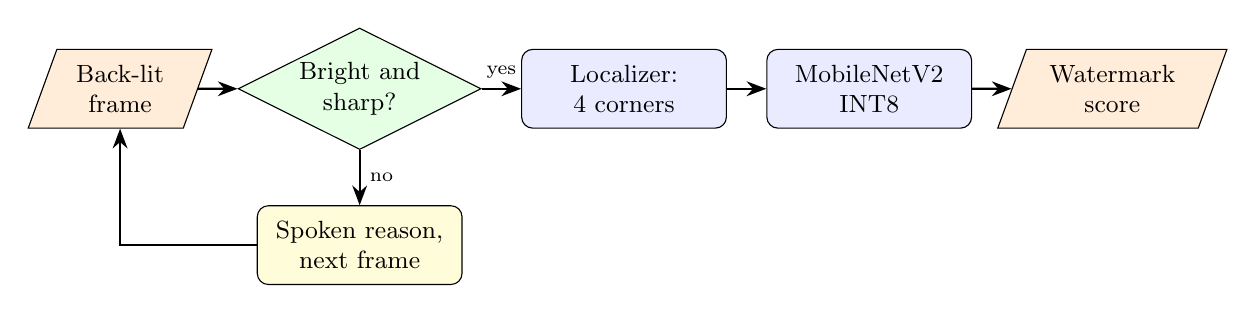
\begin{tikzpicture}[node distance=0.45cm and 0.5cm]
  \node[io] (f) {Back-lit\\frame};
  \node[decision, right=of f] (q) {Bright and\\sharp?};
  \node[block, right=of q] (loc) {Localizer:\\4 corners};
  \node[block, right=of loc] (cls) {MobileNetV2\\INT8};
  \node[io, right=of cls] (out) {Watermark\\score};
  \node[block, below=0.7cm of q, fill=yellow!15] (say) {Spoken reason,\\next frame};
  \draw[arrow] (f) -- (q);
  \draw[arrow] (q) -- node[above, font=\scriptsize]{yes} (loc);
  \draw[arrow] (loc) -- (cls);
  \draw[arrow] (cls) -- (out);
  \draw[arrow] (q) -- node[right, font=\scriptsize]{no} (say);
  \draw[arrow] (say) -| (f);
\end{tikzpicture}
\caption{Watermark check with guided capture}
\label{fig:wm_flow}
\end{figure}

\subsection{Emotion Mode}
The emotion mode finds the nearest face with the YuNet detector \cite{yunet} (an OpenCV Haar cascade is the fall-back) and classifies it into seven expressions (happy, sad, angry, surprise, fear, disgust, neutral) with an EfficientNet-V2-S network \cite{efficientnetv2} at 224$\times$224 pixels, averaging the prediction with that of the mirrored face. A FER+ model \cite{ferplus} is kept as a fall-back. When ACTION is pressed, the glass speaks the expression in Bangla. In the desktop harness the detected emotion can also change the style of the speech: slower with a short reassuring phrase for sad, fearful or angry expressions. Until 3~October 2026 the recogniser existed only in the desktop harness; it was added to the glass application as a mode on that date.

\subsection{Field Log}
\label{sec:fieldlog_method}
To study the glass in real use without loading the Raspberry Pi, every event is put on a queue and written by a background thread to \texttt{events.csv} (time, mode, button, result fields, duration); a second file, \texttt{system.csv}, records memory, CPU temperature and throttling state every 10~seconds. Saving the captured frame is optional. A report script summarises a run.

\subsection{Voice Interaction and Feedback}
All speech passes through one queue served by a worker thread, so that modes never block each other. The \texttt{TTSEngine} decides the language of each segment: if more than 25\% of the characters are in the Bangla Unicode block (U+0980--U+09FF) the segment is Bangla, otherwise English. Mixed text is split into Bangla and English runs and into sentences with a 0.15-second pause between them. Piper \cite{piper} is used for English when the binary and a voice model exist. Bangla is spoken with espeak-ng \cite{espeakng} at 135 words per minute, with a lower pitch and a small gap between words for clarity, because the only prebuilt Piper program for the Pi cannot use the public Bangla voice. In the desktop harness on Windows, Bangla is spoken with an online voice and English with the Windows speech engine. The queue holds at most five messages; older ones are dropped so that the user always hears current information.

\subsection{Overall System Flow and Logic}
Figure~\ref{fig:flow} shows the control flow of the application. The program runs several threads: the main thread, a camera thread that always keeps the latest frame, the speech worker, the object-scanning loop, an inference thread for ACTION requests, and GPIO interrupt threads. An \texttt{\_inferring} flag prevents two heavy OCR or currency jobs from running at the same time.

\begin{figure}[H]
\centering
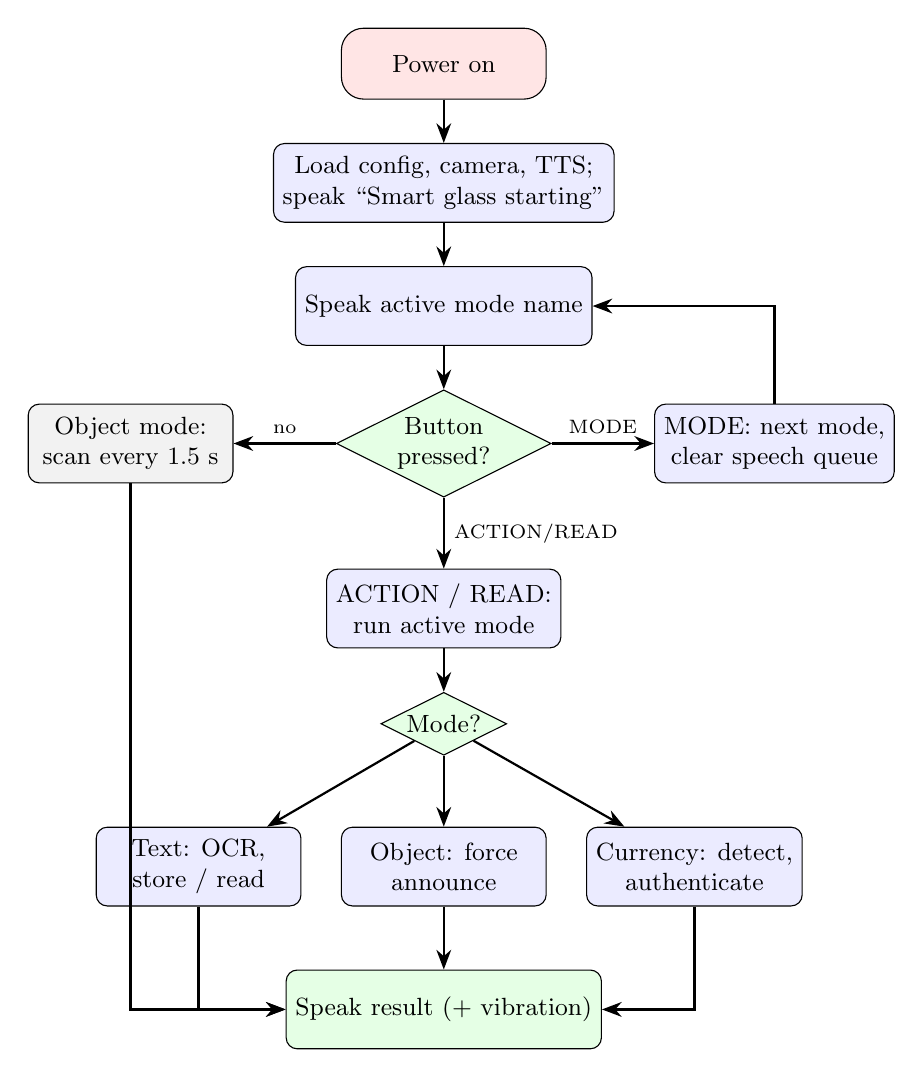
\begin{tikzpicture}[node distance=0.55cm]
  \node[startstop] (start) {Power on};
  \node[block, below=of start] (init) {Load config, camera, TTS;\\speak ``Smart glass starting''};
  \node[block, below=of init] (announce) {Speak active mode name};
  \node[decision, below=of announce] (btn) {Button\\pressed?};
  \node[block, right=1.3cm of btn] (mode) {MODE: next mode,\\clear speech queue};
  \node[block, below=0.9cm of btn] (act) {ACTION / READ:\\run active mode};
  \node[decision, below=of act] (which) {Mode?};
  \node[block, below=0.9cm of which] (o2) {Object: force\\announce};
  \node[block, left=0.5cm of o2] (o1) {Text: OCR,\\store / read};
  \node[block, right=0.5cm of o2] (o3) {Currency: detect,\\authenticate};
  \node[block, below=0.8cm of o2, fill=green!10] (speak) {Speak result (+ vibration)};
  \node[block, left=1.3cm of btn, fill=gray!10] (loop) {Object mode:\\scan every 1.5 s};
  \draw[arrow] (start) -- (init);
  \draw[arrow] (init) -- (announce);
  \draw[arrow] (announce) -- (btn);
  \draw[arrow] (btn) -- node[above, font=\scriptsize]{MODE} (mode);
  \draw[arrow] (mode) |- (announce);
  \draw[arrow] (btn) -- node[right, font=\scriptsize]{ACTION/READ} (act);
  \draw[arrow] (act) -- (which);
  \draw[arrow] (which) -- (o1);
  \draw[arrow] (which) -- (o2);
  \draw[arrow] (which) -- (o3);
  \draw[arrow] (o1) |- (speak);
  \draw[arrow] (o2) -- (speak);
  \draw[arrow] (o3) |- (speak);
  \draw[arrow] (loop) |- (speak);
  \draw[arrow] (btn.west) -- node[above, font=\scriptsize]{no} (loop.east);
\end{tikzpicture}
\caption{Overall control flow of Savior Glass}
\label{fig:flow}
\end{figure}


\section{Methodology: Building Savior Glass}
\label{sec:method}

The development of Savior Glass followed an iterative methodology in four phases: requirement analysis, data engineering and model development, system integration, and evaluation.

\subsection{Requirement Analysis}
The requirements were derived from the review of existing systems (Chapter~\ref{chap:literature}) and from the situation of visually impaired people in Bangladesh: the device must work offline, speak Bangla, read Bangla and English, recognise Taka notes, help with counterfeit notes, and be usable without a screen. These requirements defined the modes, the button interface and the choice of offline models.

\subsection{Data Engineering and Model Development}
Each vision task was developed as a separate machine learning problem with its own dataset, training procedure and held-out evaluation:
\begin{itemize}[noitemsep]
    \item \textbf{Currency detection:} a copy-paste compositing pipeline generated a large, automatically labelled detection dataset from clean note images and real backgrounds, and a COCO-pretrained YOLOv8s was fine-tuned on it (Figure~\ref{fig:method_pipeline}).
    \item \textbf{Currency authentication:} a CNN+ViT baseline was trained on six views; after observing its collapse with fewer views, the prefix-robust protocol was designed and compared against it on the same note-disjoint split. After the serial-number audit, the main methods were retrained and compared on a print-disjoint split, together with the watermark check and ResNet-50 baselines \cite{resnet}.
    \item \textbf{Emotion recognition:} several backbones were fine-tuned on the official RAF-DB training set and compared on the official test set.
    \item \textbf{Text reading:} EasyOCR was kept as the engine, and the pipeline around it was built in seven steps on a new benchmark (Section~\ref{sec:ocr_bench_data}).
    \item \textbf{Objects:} a COCO-pretrained YOLOv8 was used without retraining and evaluated on a COCO subset.
\end{itemize}

\begin{figure}[H]
    \centering
    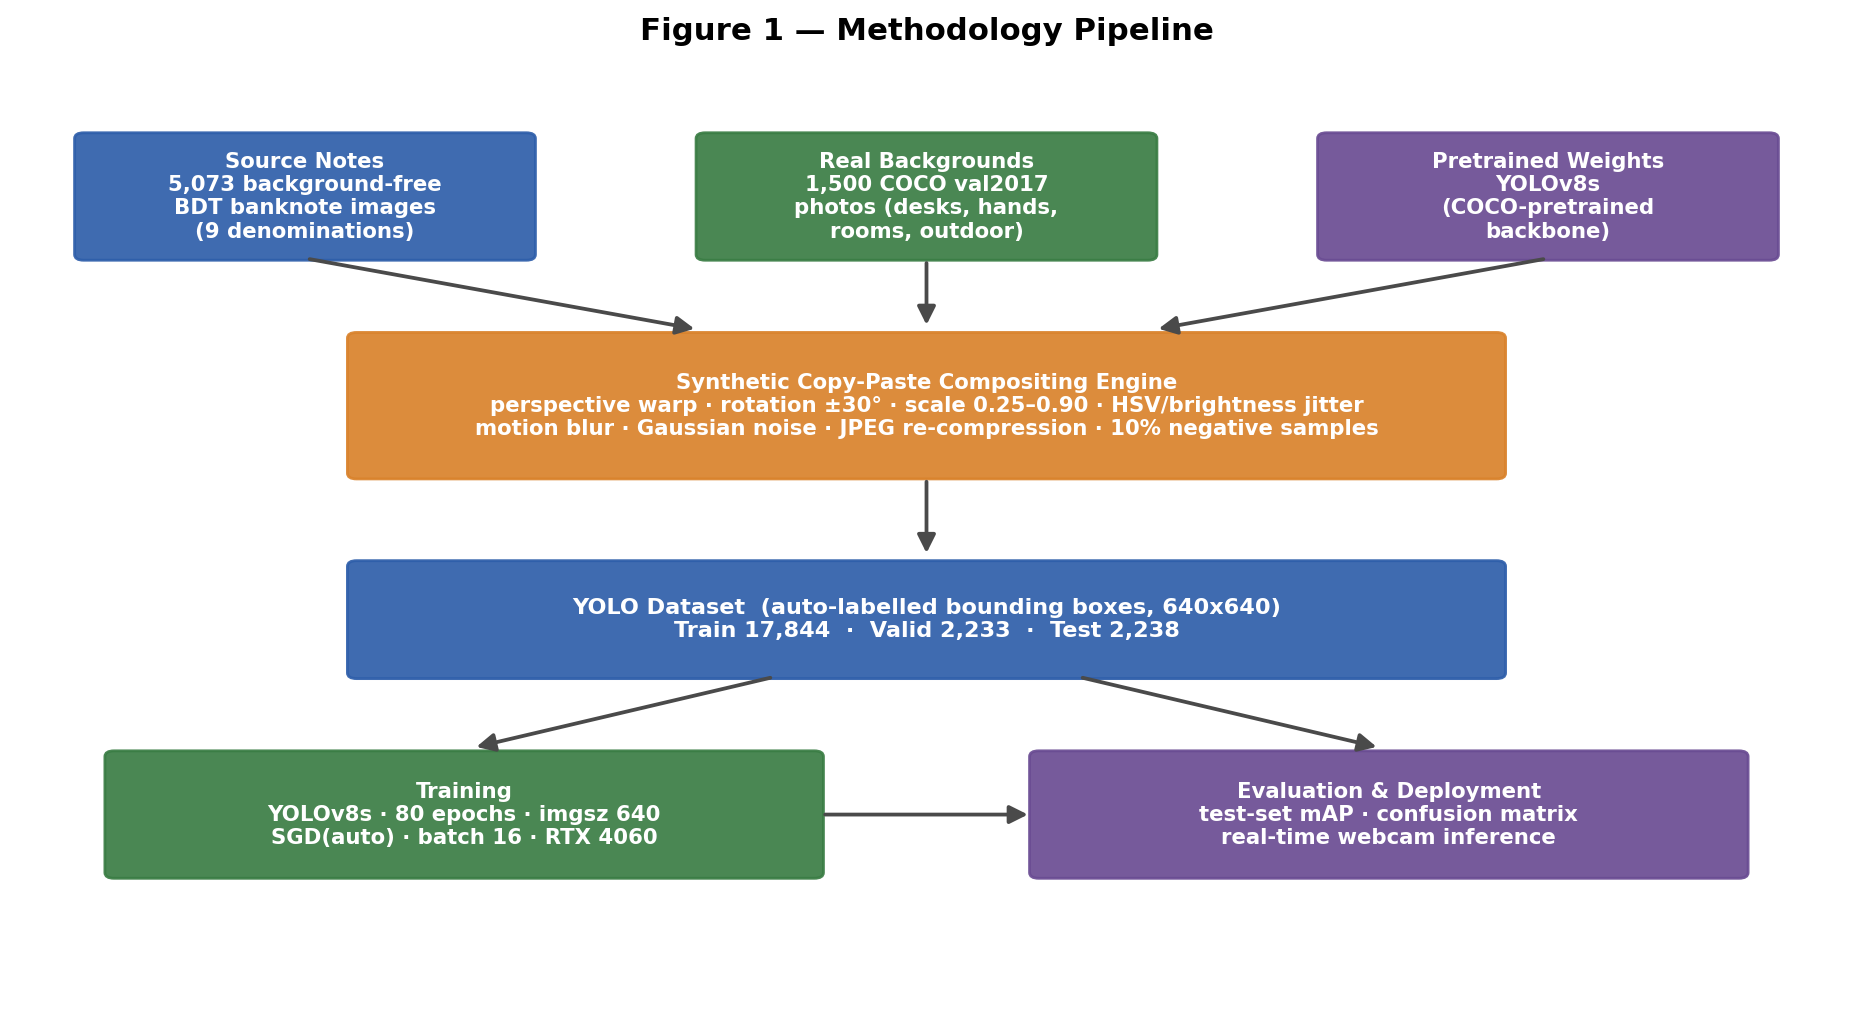
\includegraphics[width=0.9\textwidth]{fig_methodology.png}
    \caption{Currency detection methodology: source notes, COCO backgrounds and COCO-pretrained YOLOv8s weights feed the compositing engine, which produces the labelled dataset used for training, evaluation and deployment}
    \label{fig:method_pipeline}
\end{figure}

\subsubsection*{Prefix-Robust Multi-View Training}
A model trained with all six views on every sample sees only one ``number of views'' during training. At test time a blind user may capture only one or two views. This is a distribution shift in the number of views. The prefix-robust multi-view training (PRMVT) protocol removes it by sampling, for every training batch, a random prefix of the ordered views, so that every view count from 1 to 6 has positive probability during training. The protocol has two stages:
\begin{enumerate}[noitemsep]
    \item Six epochs of mixed view dropout with a per-view gate, batch normalisation per view count, an auxiliary single-view loss and a light contrastive loss.
    \item Three epochs of fine-tuning at learning rate $3\times10^{-4}$, where half of the batches use all six views so that six-view accuracy is not lost.
\end{enumerate}
The checkpoint is selected by the mean validation accuracy over one to six views; the test split is never used for selection. A simpler variant, the same network with one shared batch normalisation and prefix sampling only, was added later as a controlled comparison and turned out to be the most accurate (Section~\ref{sec:auth_results}).

\subsection{System Integration}
The trained models were integrated as modes of the glass application. Integration was first done on a Windows laptop with a webcam through a preview window, where the keyboard keys M, A, R, +, $-$ and Q replace the buttons, and then deployed on the Raspberry Pi~5 with a deployment script and a systemd service.

\subsection{Evaluation Protocol}
\label{sec:protocol}
The same rules were applied to every experiment:
\begin{itemize}[noitemsep]
    \item \textbf{Three splits.} Models are trained on the training split. Every choice (checkpoint, threshold, parameter, which method to adopt) is made on the validation split. The test split is read once for a finished method and is never used for a choice.
    \item \textbf{Split by physical unit.} Notes, writers and, for OCR, phrases and fonts are kept in one split only.
    \item \textbf{Three seeds.} Trained models are repeated with seeds 42, 43 and 44, and the mean and standard deviation are reported.
    \item \textbf{Paired tests.} Two methods on the same test items are compared with the exact McNemar test \cite{mcnemar1947} or, for error rates per image, the Wilcoxon signed-rank test \cite{wilcoxon1945}; families of tests are corrected with Holm's method \cite{holm1979}. Proportions are given with Wilson 95\% intervals \cite{wilson1927}.
    \item \textbf{Negative results.} A method that does not help is reported and not adopted, even if it looks better on the test split.
\end{itemize}
The metrics per module are:
\begin{itemize}[noitemsep]
    \item \textbf{Currency detection:} precision, recall, mAP@0.5 and mAP@0.5:0.95 on held-out composites; top-1 denomination accuracy on independent photographs.
    \item \textbf{Authentication:} accuracy for 1 to 6 views on the note-disjoint and the print-disjoint split; expected calibration error (ECE) \cite{guo2017calibration}; robustness under image corruptions; for the deployed policy, the number of counterfeits passed as genuine and of genuine notes confirmed.
    \item \textbf{Emotion:} accuracy, macro precision, recall and F1 on the official RAF-DB test set.
    \item \textbf{OCR:} character error rate (CER) and word error rate (WER), the edit distance \cite{levenshtein1966} between the recognised text and the ground truth divided by the length of the ground truth, after Unicode NFC normalisation.
    \item \textbf{Objects:} mAP@0.5 on a 250-image COCO val2017 subset.
    \item \textbf{Speed:} median and 95th-percentile time per call over 100 calls on the Raspberry Pi~5, and memory, temperature and throttling state during a 30-minute mixed run.
\end{itemize}
An append-only database (\texttt{research\_results/experiments.json}, 204 experiments in 11 comparison groups) records each experiment with its result file, and a claim registry links the 298 numerical claims of the project to their files; a script checks that each claimed value equals the value in the file.
All numbers in Chapter~\ref{chap:results} are copied from these files. Measurements that do not yet exist are marked as not measured.

\clearpage
\chapter{Implementation Process}
\label{chap:implementation}

\section{Design Overview}

The implementation of Savior Glass was guided by usability for people without sight, by the limited computing power of a Raspberry Pi, and by the need to work without the internet. The system was not designed as a single large model; instead, each function is a small, replaceable mode that uses the best available offline model and falls back to a simpler method if a model is missing. The work progressed in four stages: a user-centred interaction design, a desktop prototype with a webcam, deployment and measurement on the Raspberry Pi~5, and a first hands-on test of the glass.

\subsection{User-Centred Design}
A person who cannot see the device must be able to find every control by touch and must never need a screen. For this reason the glass uses five physical buttons with distinct positions, confirms every action with speech, and speaks the name of the mode after every mode change. Heavy tasks run only on request, so that the user decides when the device speaks. Messages are short, in Bangla, and can be repeated with the READ button in text mode. When the device cannot do what was asked, it says why: ``no note found, hold it in front of the camera'', ``hold the note closer to the light'', ``no face found''.

\subsection{Prototype Development Environment}
Most development and all model training were done on Windows~11 laptops with NVIDIA GPUs. The authentication, watermark, emotion and OCR experiments, and all evaluations reported in this thesis, were run on an RTX~3050 Laptop GPU with CUDA~12.4 and PyTorch~2.6 \cite{pytorch}. The same Python code runs on the Raspberry Pi~5; only the camera, button and audio back-ends differ.

\section{Hardware Implementation}

\subsection{Component Assembly}
The camera module is mounted above the bridge of the spectacle frame so that it points where the user's face points. In the first prototype the Raspberry Pi~5 is tied to the right temple of the frame and the ribbon cable loops over the head from the camera to the board (Figure~\ref{fig:prototype}); Figure~\ref{fig:worn} shows it being worn. In the intended design the cable runs along the temple to a separate enclosure, which carries the board and the button pad, the earphone connects to the audio output, and the vibration motor sits in the enclosure so that the user can feel it in the hand or pocket.

\begin{figure}[H]
    \centering
    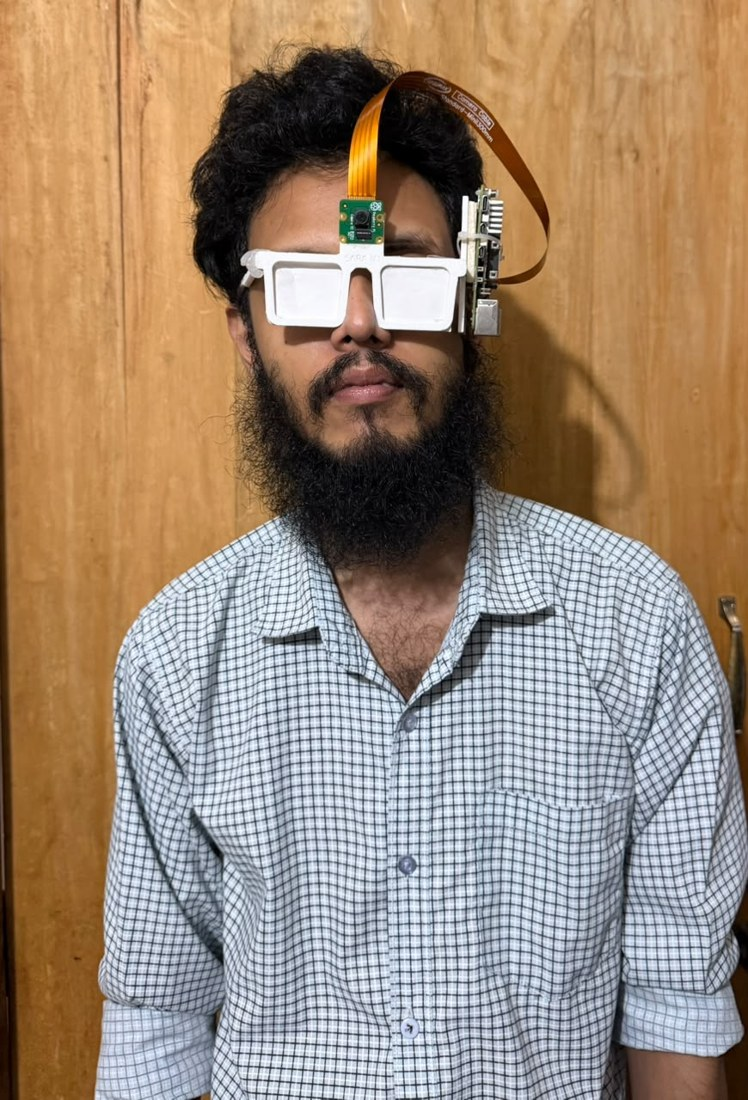
\includegraphics[height=6.2cm]{worn_front.jpg}
    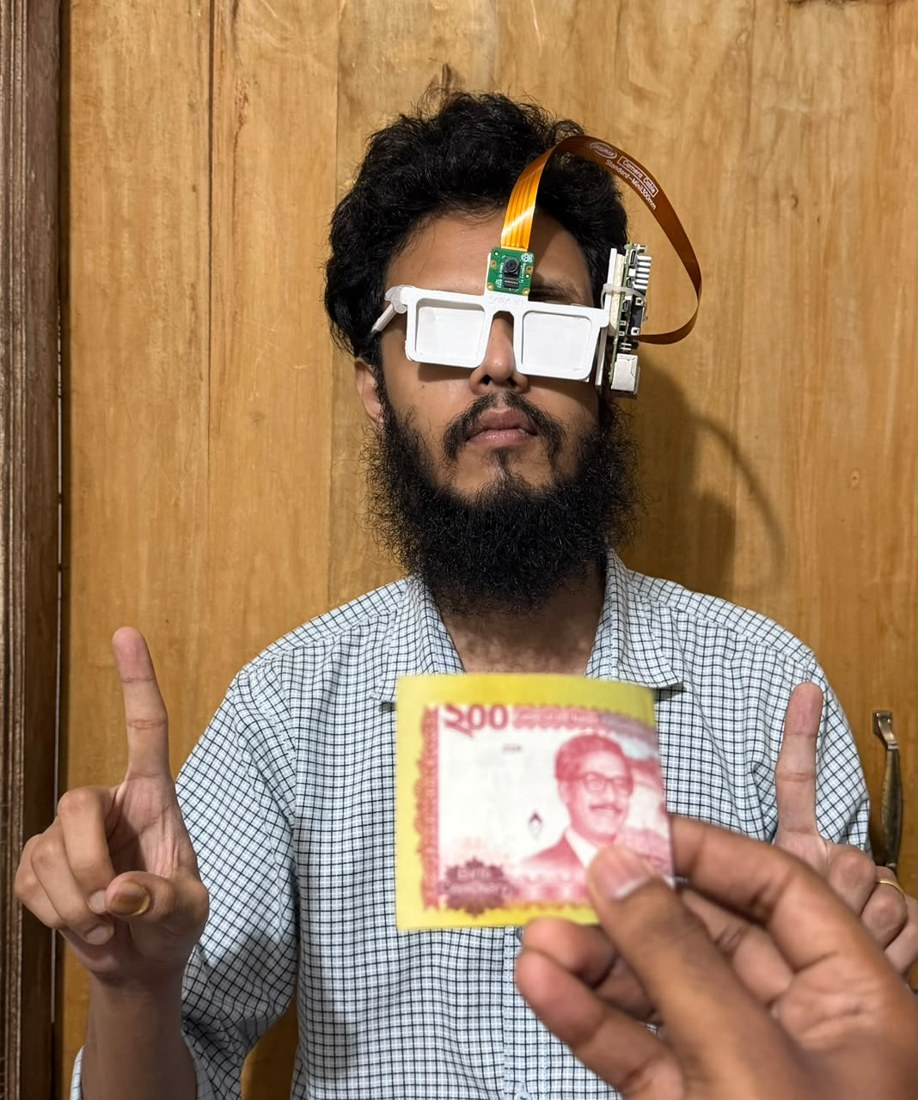
\includegraphics[height=6.2cm]{worn_200.jpg}
    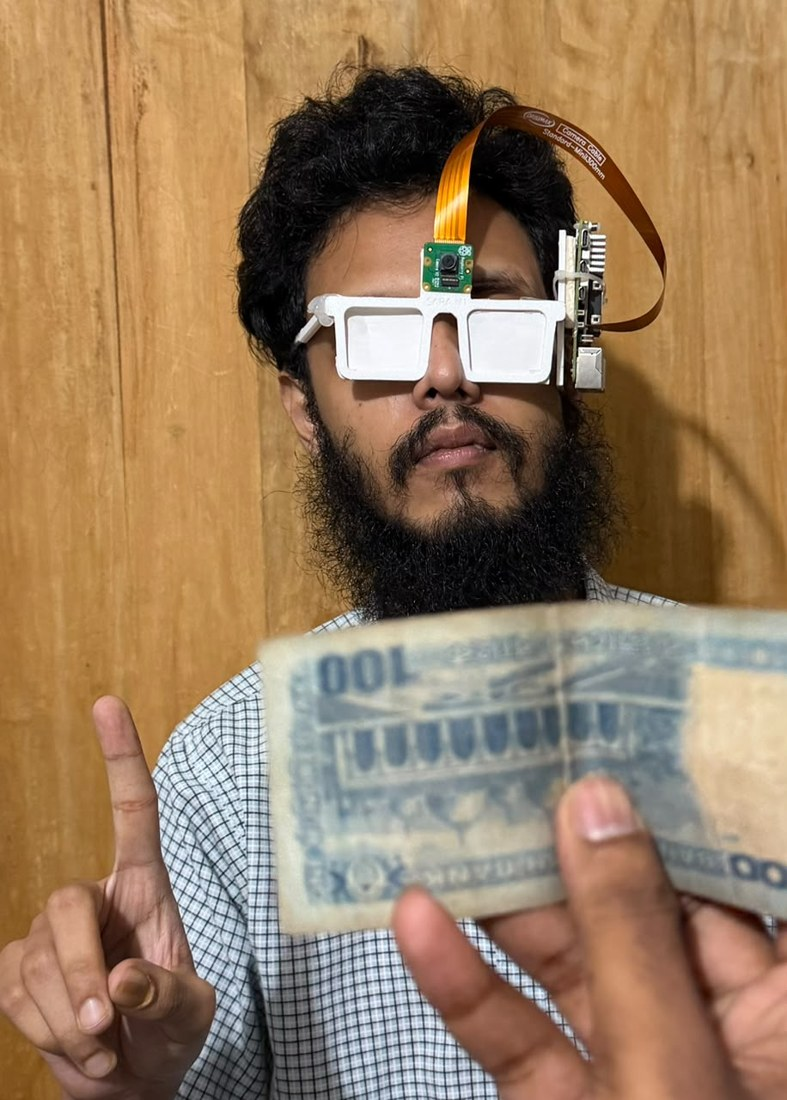
\includegraphics[height=6.2cm]{worn_100.jpg}
    \caption{The first prototype worn during a trial session. A 200 Taka and a 100 Taka note are held in front of the camera for the currency mode. The photographs are used with the wearer's consent.}
    \label{fig:worn}
\end{figure}

\subsection{Connectivity and Wiring}
\subsection*{1. Raspberry Pi~5 Power}
The Raspberry Pi~5 is powered through its USB-C port from a power bank. The system starts automatically when power is connected.

\subsection*{2. Camera Module~2}
The camera is connected to the CSI connector and read with Picamera2. On the Raspberry Pi~5 the OpenCV capture interface opened the camera device but received no frames, so the camera manager now tries Picamera2 first, then OpenCV, and finally scans the video devices while skipping the Pi's internal image-processing nodes. If the camera is already in use by another program, the manager stops with a message that says so. A USB webcam is selected with \texttt{CAMERA\_BACKEND} and \texttt{CAMERA\_INDEX}; the frame size is set with \texttt{CAMERA\_WIDTH} and \texttt{CAMERA\_HEIGHT}.

\subsection*{3. Push-Buttons}
Each button connects one GPIO pin (BCM 17, 27, 24, 22, 23) to ground. The pins are configured as inputs with internal pull-up resistors, and a falling edge generates an interrupt that is debounced in software for 250~ms using the \texttt{rpi-lgpio} library. The library creates a notification pipe in its working directory; because the project was kept on a FAT-formatted USB drive, which cannot hold pipes, the working directory of the library is set to the system's temporary folder. A pin that is already claimed by another process produces an error message with instructions instead of a stack trace.

\subsection*{4. Vibration Motor}
The vibration motor is driven with PWM from BCM pin 13. Patterns are defined as lists of (on, off) durations in milliseconds; a detected note gives one pulse of 50~ms.

\subsection*{5. Audio}
Speech is sent to the default ALSA device with \texttt{aplay}; the volume is changed with \texttt{amixer}. Piper produces 16-bit mono PCM at 22,050~Hz, which is streamed directly to \texttt{aplay} without writing a file.

\section{Software Deployment and Functional Integration}

\subsection{Environment Setup and Libraries}
The software stack is summarised in Table~\ref{tab:libraries}. On the Raspberry Pi, the deployment script \texttt{scripts/deploy\_pi5.sh} installs the system packages (libcamera, Picamera2, espeak-ng, ALSA utilities, OpenBLAS), creates a Python virtual environment, installs the Python requirements, the Piper ARM64 program and an English voice, and copies the model files. The virtual environment is created in the user's home folder with access to the system packages: Picamera2 is a system package, and the FAT-formatted drive that holds the project cannot store the symbolic links a virtual environment needs. A pre-flight script (\texttt{scripts/pi5\_preflight.py}) then checks that every model and library is present before the application is started.

\begin{table}[!htbp]
\centering
\caption{Main libraries and tools used in Savior Glass}
\label{tab:libraries}
\begin{tabular}{|p{3.6cm}|p{10.2cm}|}
\hline
\textbf{Library / Tool} & \textbf{Use in the project} \\ \hline
Python 3 & Application language \\ \hline
OpenCV \cite{opencv} & Pre-processing, YuNet or Haar face detection, SIFT registration, USB camera capture \\ \hline
Picamera2 & Capture from the Pi camera \\ \hline
PyTorch, torchvision & Training and inference of MobileNetV3, EfficientNet-V2-S, TinyViT models \\ \hline
Ultralytics YOLOv8 & Object and Taka detection, training, export to ONNX and TorchScript \\ \hline
ONNX Runtime & Inference of the INT8 Taka detector, the watermark localizer and classifier, FER+ fall-back \\ \hline
EasyOCR & Bangla and English text recognition \\ \hline
HarfBuzz, FreeType & Correct shaping of Bangla text in the OCR benchmark images \\ \hline
Tesseract, PaddleOCR, KenLM, SymSpell & OCR engines and correctors compared in the benchmark \\ \hline
sounddevice, SpeechRecognition & Microphone capture and speech recognition in the voice study tool \\ \hline
Piper, espeak-ng & Offline neural and formant speech synthesis \\ \hline
rpi-lgpio & GPIO buttons and PWM on Raspberry Pi~5 \\ \hline
pytorch-grad-cam & Grad-CAM visual explanations \\ \hline
systemd & Start at boot and automatic restart \\ \hline
\end{tabular}
\end{table}

\subsection*{Integration Stages}
Integration was carried out step by step:
\begin{enumerate}[noitemsep]
    \item Camera and speech alone: live frames and spoken test sentences.
    \item Button handling: mode cycling with spoken mode names.
    \item Each mode added and tested separately in the Windows harness.
    \item Concurrency: object scanning in parallel with on-demand OCR and currency, protected by an inference flag.
    \item Packaging: deployment script, systemd service and logging with rotation (5~MB, 3 backups).
    \item Deployment on the Raspberry Pi~5 and benchmark of every mode.
    \item Field log, live algorithm panel and study tools.
\end{enumerate}

\section*{Core Implementation Modules}

\subsection*{Camera Manager}
The \texttt{CameraManager} runs a background thread that reads frames continuously and keeps only the most recent one. Modes always receive a fresh frame, and a slow OCR call never causes a backlog of old frames.

\subsection*{Mode Switching}
Loading a model takes one to two seconds, which is too long to wait in silence. When MODE is pressed, the name of the mode is spoken at once and the model is loaded and warmed up in a background thread; a lock prevents two models from loading at the same time, and the currency mode is preloaded when the application starts. On the laptop CPU this reduced the first currency check after a mode change from 661~ms to 43~ms.

\subsection*{Language Detection and Speech Segmentation}
The speech engine decides the language of each piece of text by counting Bangla characters, and splits mixed-script text into runs that are spoken with the correct voice:

\begin{lstlisting}[language=Python]
def detect_language(text: str) -> str:
    """Return 'bn' if >25% of non-space characters are Bangla, else 'en'."""
    stripped = text.replace(" ", "")
    if not stripped:
        return "en"
    bangla_count = len(_BANGLA_RE.findall(stripped))
    return "bn" if (bangla_count / len(stripped)) > 0.25 else "en"
\end{lstlisting}

Speaking a mixed Bangla--English sentence as one block forces the wrong voice onto half of it, which made early OCR output sound garbled. Splitting on script boundaries fixed this while keeping the original reading order.

\subsection*{Text Reading with EasyOCR}
The OCR mode loads the EasyOCR reader for Bangla and English lazily on first use, because it needs about 600~MB of memory; on a machine with a GPU it uses the GPU, on the Pi the CPU. The frame is contrast-enhanced with CLAHE and read once with the tuned settings. The step that matters most is the selection of the main text block, shown below as it is in the code. It starts from the box with the largest product of height and confidence and repeatedly adds boxes that have a similar height and lie within one and a half text heights of the block:

\begin{lstlisting}[language=Python]
def dominant_block(det, min_conf=0.2, h_ratio=0.6, gap=1.5):
    boxes = [b for b in _boxes(det) if b["c"] >= min_conf]
    if not boxes:
        return []
    seed = max(boxes, key=lambda b: b["h"] * b["c"])
    block, rest = [seed], [b for b in boxes if b is not seed]
    grown = True
    while grown:
        grown = False
        for b in list(rest):
            hs = float(np.median([x["h"] for x in block]))
            if not (h_ratio <= b["h"] / max(hs, 1.0) <= 1 / h_ratio):
                continue                      # different text size
            if any(b["x0"] - x["x1"] < gap * hs and
                   x["x0"] - b["x1"] < gap * hs and
                   b["y0"] - x["y1"] < gap * hs and
                   x["y0"] - b["y1"] < gap * hs for x in block):
                block.append(b)               # touches the block
                rest.remove(b)
                grown = True
    return block
\end{lstlisting}

The boxes of the block are then grouped into lines by their vertical centre, each line is sorted from left to right, and the clean-up rules are applied. The text is spoken once directly after capture and stored, so that READ can repeat it.

EasyOCR enlarges the image towards a canvas size before detection. A canvas of 640 pixels makes OCR about three times faster on the Pi than the default of 2,560, but on a selection set of phrases that the OCR pipeline had never seen it missed the pre-set margin of 0.5 points (13.84\% against 13.29\% CER, Wilcoxon $p = 0.48$), so the default stays at 2,560 and the faster setting is available through \texttt{OCR\_CANVAS\_SIZE}.

\subsection*{Object Detection with YOLOv8}
The detection loop runs only in object mode. Every 1.5 seconds it takes the latest frame, resizes it to 320$\times$240, runs YOLOv8 with confidence 0.50, keeps the three most confident unique classes whose cooldown has expired, translates them to Bangla with \texttt{labels\_bn.json}, and queues a sentence of the form ``in front: \textit{object 1}, \textit{object 2}''. Pressing ACTION forces the next scan to ignore the cooldown.

\subsection*{Currency Detection and Authentication}
The currency mode first runs the YOLOv8s Taka detector. The logic that follows was shaped by three failures. An earlier version fell back to a colour guess when the detector found nothing, and announced wrong denominations; the colour guess is now used only when no detector is installed. An earlier version announced every detection, and named 1 Taka notes, which the detector does not know, as other notes; a detection is now announced only at a confidence of at least 0.60. And an earlier version spoke ``genuine'' or ``counterfeit'' from one crop of the note, which was wrong on 20--59\% of genuine whole-note photographs (Section~\ref{sec:jaal_deployed}); it was first switched off and then replaced by the safe policy. The simplified logic is:

\begin{lstlisting}[language=Python]
def process_frame(self, frame):               # simplified
    hits = self.detect_live(frame)            # YOLOv8s Taka + safe check
    if hits and hits[0]["conf"] < config.CURRENCY_ANNOUNCE_CONF:
        return NOT_SURE_HOLD_CLOSER           # possibly an unknown note
    if hits:
        self._buzz("detect")
        if hits[0]["auth"] in ("likely_genuine", "check_by_hand"):
            return hits[0]["text"]            # value + safe verdict
        return hits[0]["text"] + CHECK_NOT_DONE   # other denominations
    if self._yolo is not None:
        return NOTE_NOT_FOUND_MESSAGE
    ...                                       # no detector: colour fall-back
\end{lstlisting}

For a 500 or 1,000 Taka note the four view windows are cut from the detected box and scored, and the text becomes the denomination followed by ``likely genuine'' or ``check by hand''. When the watermark check is switched on (the default on the Pi), the capture guide then asks the user to hold the note up to a light and runs the watermark path of Section~\ref{sec:watermark_method}. Every watermark check is written to a study log with the participant, the condition (guided or not), the time, the rejected frames and the outcome.

The detector is also used in a live desktop application that draws boxes on the webcam image and speaks the detected note when SPACE is pressed (Figure~\ref{fig:webcam}). Frames darker than a mean intensity of 80 are brightened with a gain of 3.0 and a gamma of 0.5 before detection, which fixed a failure observed in dim rooms.

\begin{figure}[H]
    \centering
    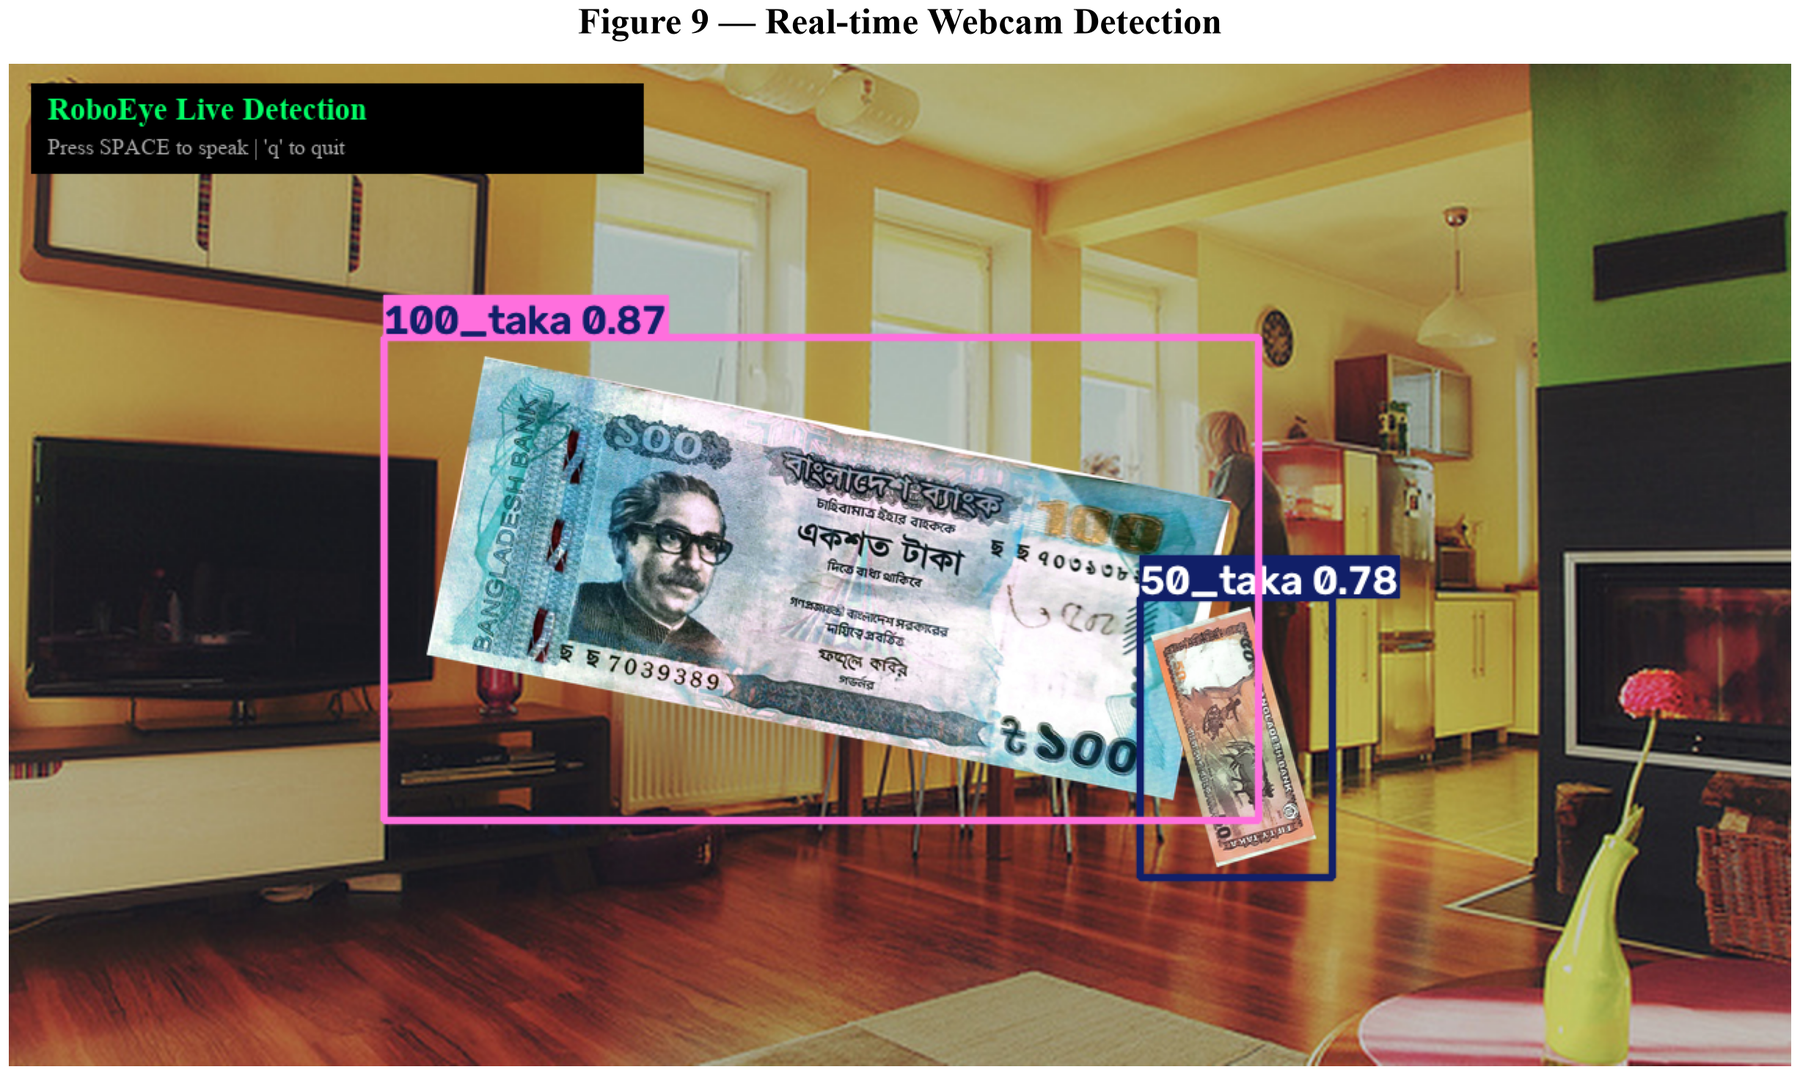
\includegraphics[width=0.85\textwidth]{fig9_webcam_detection.png}
    \caption{Live detection application: a 100 Taka and a 50 Taka note are detected with confidence 0.87 and 0.78 in an indoor scene}
    \label{fig:webcam}
\end{figure}

To check that the detector looks at meaningful parts of the note, Grad-CAM \cite{gradcam} heat maps were produced. Figure~\ref{fig:gradcam} shows that the activation concentrates on the portrait and the denomination numerals rather than on the background.

\begin{figure}[H]
    \centering
    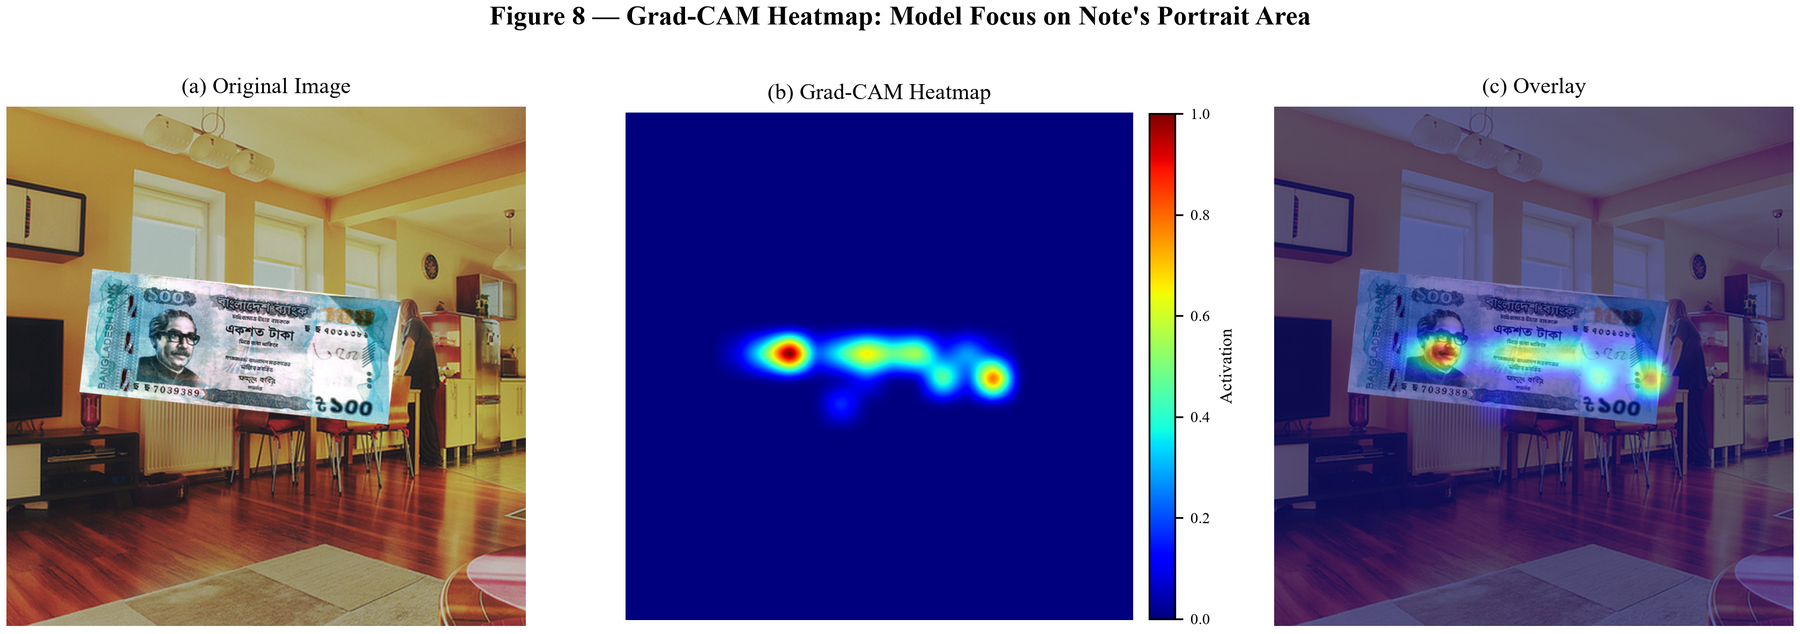
\includegraphics[width=\textwidth]{fig8_gradcam.png}
    \caption{Grad-CAM explanation for a 100 Taka note: (a) input, (b) heat map, (c) overlay. The model focuses on the portrait and numeral regions.}
    \label{fig:gradcam}
\end{figure}

\subsection*{Model Export for the Edge}
The Taka detector was exported to TorchScript, ONNX and INT8-quantised ONNX. The first INT8 export quantised the whole network, including the detection head; its class scores collapsed (highest score 0.007) and it detected no note on the test images, so it was discarded. The INT8 model now used is statically quantised with ONNX Runtime, calibrated on 200 validation images, with the detection head and the first convolution kept in 32-bit floating point. On the full synthetic test split it matches the FP32 ONNX model (mAP@0.5 0.995 for both; mAP@0.5:0.95 0.823 against 0.821), and the file is 18.0~MB compared with 22.5~MB for the PyTorch weights.

\subsection*{Emotion Mode}
The emotion mode detects the nearest face with YuNet, crops and resizes it to 224$\times$224, and classifies it with EfficientNet-V2-S, averaging the prediction with that of the mirrored face. It speaks one sentence, ``the person in front looks happy'' (in Bangla), or says that no face was found and that the camera should be pointed at a face. The model file is 82~MB. Until 3~October 2026 emotion recognition ran only in the desktop harness, where it adapted the speaking style; an earlier project report described it as working on the glass, which was wrong, and the mode was added after the first field test showed that it was missing. On the glass the camera faces outward, so the mode describes the person in front of the user, not the user.

\subsection*{Optional Online Scene Description}
The online mode sends the current frame to a cloud vision--language model and speaks a short Bangla or English description. It supports the Anthropic and the OpenAI API, requires an internet connection and an API key, and is never used by the other modes. Its accuracy and latency have not been measured: the account supplied for the test had no credit, and the evaluation script returned an error for every request.

\subsection*{Field Log and Live Algorithm Panel}
The field logger writes two CSV files per run. \texttt{events.csv} has one row per event with the columns time, event, mode, latency, result, denomination, confidence, verdict, score, language and detail; \texttt{system.csv} has the CPU temperature, throttling state, load, free memory and the memory of the application every 10~seconds. Rows are put on a queue and written by a separate thread, so logging does not slow the modes; if the queue is full, the event is counted as dropped. For demonstrations and debugging, the preview window has a panel (key L) that runs every model on the current picture and shows its output and time.

\subsection*{Voice Study Tool}
For the user study, a session runner asks the participant's name by voice, lets the participant use the glass, and, when the experimenter presses D, asks six yes/no questions in Bangla (ease of use, clarity of speech, help with currency, help with reading, trust, willingness to use daily). Answers are spoken. The microphone is read at its native sample rate, recording starts after 0.2~seconds of sound and stops after 1~second of silence, so that a click is not taken for an answer; the recording is sent to an online speech recogniser in Bangla and, if no yes or no is found, in English, and every alternative transcription is searched for a yes or no word. The experimenter can also answer with the Y and N keys. Each session receives an identifier (P001, P002, \dots) and is saved automatically with the recordings, the recognised text and whether each answer came by voice or key. This tool needs the internet and runs on the laptop, not on the Pi.

\subsection*{Start at Boot}
The glass runs as a systemd service so that it starts without a keyboard or screen and restarts automatically after a crash:

\begin{lstlisting}
[Service]
Type=simple
User=pi
WorkingDirectory=/home/pi/smart-glass
ExecStart=/home/pi/smart-glass-env/bin/python3 /home/pi/smart-glass/main.py
Restart=on-failure
RestartSec=5
SupplementaryGroups=gpio audio video
\end{lstlisting}

\subsection{Windows Development Harness}
Because hardware testing is slow, the same application runs on a Windows laptop with a webcam and a preview window. The keys M, A, R, +, $-$ and Q replace the five buttons and the power switch, L opens the algorithm panel, and in a study session D ends the use phase and N starts the next participant. The window shows the camera image, the detections and a status panel. On Windows, English is spoken with the system speech engine and Bangla with an online voice, because the system engine cannot speak Bangla; offline Bangla speech is tested on the Pi with espeak-ng.

\subsection{Error Handling and Functional Validation}
Every model is loaded inside a \texttt{try} block. If a model file is missing, the mode logs a warning and falls back to the next stage instead of crashing: the watermark window falls back from the learned localizer to SIFT registration, OCR from EasyOCR to Tesseract, object detection from YOLOv8s to YOLOv8n, speech from Piper to espeak-ng, and emotion recognition from EfficientNet-V2-S to FER+. One such fall-back had hidden a fault: when Piper failed on the Pi it produced no sound at all instead of falling back, which was found and fixed during the Pi benchmark. Camera failures produce a spoken message (``camera not ready''). The speech queue drops old messages when full, so that a burst of detections never delays the user by more than a few seconds.

\section{Testing and Calibration}
Testing proceeded from single functions to the complete system.

\subsubsection{Camera and OCR Testing}
The OCR pipeline was first tuned by comparing recognition confidence on rendered words. This was replaced by the benchmark of Section~\ref{sec:ocr_bench_data}, in which every choice is made on validation phrases and fonts and scored by the error rate, not by the engine's own confidence.

\subsubsection{Currency Detector Testing}
The detector was evaluated on held-out composites, run live twice for about five minutes each without errors, checked with diagnostic webcam captures in dim light (mean brightness 40 raised to 174 by the brightening step), and evaluated on independent photograph collections.

\subsubsection{Authenticator Testing}
All authentication models were evaluated with 1, 2, 3, 4, 5 and 6 views on the same note-disjoint test split, with 13 image corruptions and with calibration metrics, and the main models again on the print-disjoint split. The path used by the application (localizer and INT8 classifier) was checked against the research path on the 222 test photographs and made the same decision on 99.1\% of them.

\subsubsection{Voice and Audio Calibration}
The espeak-ng voice was slowed from the default 150 to 135 words per minute, the pitch was lowered from 50 to 45, and a word gap was added, which made Bangla speech easier to follow. A 0.15-second pause between segments separates sentences.

\subsubsection{End-to-End Interaction Testing}
Complete sequences (boot, mode change, capture, read, currency detection, volume change) were run in the Windows harness and then on the Raspberry Pi~5, where every mode was timed (Section~\ref{sec:pi5}). A first hands-on test of the glass followed (Section~\ref{sec:field_test}). A structured test with visually impaired users has not yet been carried out.

\section{Deployment Problems on the Raspberry Pi~5}
\label{sec:deploy_problems}
Bringing the application from the laptop to the Pi exposed problems that no laptop test could show. They are listed in Table~\ref{tab:deploy} because each of them stopped the glass from starting.

\begin{table}[!htbp]
\centering
\caption{Problems met when deploying on the Raspberry Pi~5, and their fixes}
\label{tab:deploy}
\begin{tabular}{|p{4.4cm}|p{4.6cm}|p{5.0cm}|}
\hline
\textbf{Symptom} & \textbf{Cause} & \textbf{Fix} \\ \hline
Virtual environment cannot be created & Project on a FAT USB drive, which cannot hold symbolic links & Environment in the home folder, with system packages visible \\ \hline
GPIO library fails with ``file not found'' & Its notification pipe cannot be created on the same drive & Working directory of the library set to the temporary folder \\ \hline
``Camera: no frames received'' & OpenCV capture does not deliver frames from the Pi camera & Picamera2 as the first back-end \\ \hline
``Camera in use'', ``GPIO busy'' & A second copy of the application was running & Clear error message; stop the other copy \\ \hline
Missing ONNX Runtime & Not in the requirements for the Pi & Added; pre-flight check of all libraries and models \\ \hline
No sound when Piper fails & Silent failure instead of fall-back & Fall-back to espeak-ng \\ \hline
Bangla Piper voice unusable & The prebuilt ARM64 Piper cannot phonemise the Bangla voice & espeak-ng for Bangla (open problem) \\ \hline
\end{tabular}
\end{table}

\clearpage
\chapter{Dataset and Data Engineering}
\label{chap:dataset}

\section{Dataset}
Savior Glass combines several vision tasks, and each task needs its own data. Table~\ref{tab:datasets} lists every dataset used in this project, what it was used for, and how it was split. All training, validation and test splits are disjoint; where the same physical note or person could appear in more than one image, the split was made by the physical unit (note or writer), not by image. For counterfeit notes even that is not enough, as Section~\ref{sec:serial_audit} shows.

\begin{table}[!htbp]
\centering
\caption{Datasets used in this project}
\label{tab:datasets}
\begin{tabular}{|p{3.2cm}|p{3.4cm}|p{3.1cm}|p{4.2cm}|}
\hline
\textbf{Dataset} & \textbf{Content} & \textbf{Task} & \textbf{Split / use} \\ \hline
BanglaTaka \cite{banglataka} & 5,073 background-free Taka photos, 9 denominations & Currency foregrounds & 80/10/10 by source note \\ \hline
COCO \cite{coco} & Natural photographs & Backgrounds; object test; OCR photo scenes & Random crops for compositing \\ \hline
Synthetic Taka detection set & 22,333 composites (this work) & Taka detection & 17,839 / 2,212 / 2,282 \\ \hline
Fresh composite test & 566 composites of test notes on other backgrounds & Taka detection & Test only \\ \hline
Bangla Money (Kaggle) & 1,536 photographs, 8 denominations; 101 photographs of 1 Taka & Taka detection & Independent test only \\ \hline
NSTU-BDTAKA \cite{nstubdtaka2024} & 186 detection images, 1,144 hand-held close-ups & Taka detection & Independent test only \\ \hline
JaalTaka \cite{jaaltaka} & 1,390 notes $\times$ 6 views = 8,340 images; 500 and 1,000 Taka & Genuine vs counterfeit & Note-disjoint 974 / 208 / 208; print-disjoint 946 / 222 / 222 \\ \hline
Bangladeshi Counterfeit Currency Image Dataset & Whole-note photographs: 1,199 genuine, 87 counterfeit (about 4 physical counterfeit notes) & Check of the deployed verdict & Test only \\ \hline
MVP-N \cite{mvpn}, ModelNet40 \cite{modelnet} & Multi-view object sets & Whether the view-count finding holds outside currency & Their own splits \\ \hline
RAF-DB \cite{rafdb} & 15,339 face images, 7 expressions & Emotion & Official 12,271 / 3,068 \\ \hline
OCR benchmark (this work) & Bangla and English phrases rendered with correct shaping; 432 images per phrase set & OCR development and test & Separate validation and test phrases and fonts \\ \hline
Ekush \cite{ekush} & 367,018 handwritten Bangla characters, 122 classes & Handwritten-letter fall-back & Writer-disjoint 2,429 / 303 / 305 writers \\ \hline
COCO val2017 subset & 250 images, 77 classes present & Object evaluation & Test only \\ \hline
\end{tabular}
\end{table}
\FloatBarrier

\subsection{Implications of These Datasets on Our Research}
The datasets define what each result means. The Taka detector is trained only on synthetic composites, so its test score on composites measures performance on data that is statistically similar to training; the raw photograph set is closer to real use. JaalTaka is split by physical note, so the authenticator is never tested on a note it has seen in training; but many of its counterfeit notes are copies of the same print, so the note-disjoint split measures the recognition of known prints, and a second, print-disjoint split is needed. All its notes come from one capture collection, so camera and session changes are not tested. RAF-DB is a standard benchmark with an official split, which allows comparison with published work. The OCR benchmark consists of rendered text, some of it placed in real photographs; it separates the effect of each pipeline step cleanly, but real signs, glare and curved packets will be harder. None of the datasets was photographed through the glass camera.

\section{Currency Detection Data Engineering}

\subsection{Source Currency Dataset (Foreground)}
The banknote images come from the BanglaTaka dataset, ``A Diverse Image Dataset for Bangladeshi Currency Recognition'', on Mendeley Data \cite{banglataka}. It contains 5,073 background-free images of Taka notes of all nine circulating denominations, captured with different mobile phones and cropped to the note (Table~\ref{tab:banglataka}). Because each image is a tight crop of one note, it is ideal foreground material for compositing.

\begin{table}[!htbp]
\centering
\caption{Per-denomination image counts in the BanglaTaka source dataset}
\label{tab:banglataka}
\begin{tabular}{|l|c|c|c|c|c|c|c|c|c|c|}
\hline
\textbf{Denomination} & 2 & 5 & 10 & 20 & 50 & 100 & 200 & 500 & 1000 & \textbf{Total} \\ \hline
\textbf{Images} & 445 & 660 & 419 & 480 & 416 & 565 & 423 & 1,243 & 422 & \textbf{5,073} \\ \hline
\end{tabular}
\end{table}

\subsection{Background Dataset}
Real backgrounds were taken from the COCO val2017 split \cite{coco}, which contains natural photographs of rooms, desks, streets, hands and outdoor scenes. We downloaded 1,500 images programmatically. Using real photographs instead of plain colours or noise, as in an earlier internal version of the pipeline, was the single most important change for generalising to real camera frames, because it forces the detector to separate the note from realistic clutter, texture and lighting.

\subsection{The Domain-Gap Problem}
A model trained only on background-free notes learns that the note fills the whole frame on a plain background. An early version of this project labelled every training image with a box covering the entire frame. It scored well on its own synthetic test set but failed to detect notes on a live webcam, where the note is small, rotated and surrounded by objects. This failure motivated the compositing redesign.

\subsection{Copy-Paste Compositing Process}
Each source note is pasted onto a randomly chosen and randomly cropped COCO background after a chain of random transformations (Figure~\ref{fig:compositing}). Because the position and size of each pasted note are known exactly, the YOLO label is computed directly from the paste geometry. For a note of pixel size $(w,h)$ pasted with its top-left corner at $(x,y)$ on a square canvas of size $S=640$:
\begin{align}
x_c &= \frac{x + w/2}{S}, \qquad y_c = \frac{y + h/2}{S}, \\
b_w &= \frac{w}{S}, \qquad\qquad\;\; b_h = \frac{h}{S},
\end{align}
where $(x_c, y_c)$ is the normalised box centre and $(b_w, b_h)$ the normalised box size. This closed-form labelling produced a fully labelled dataset with zero manual annotation.

\begin{figure}[H]
    \centering
    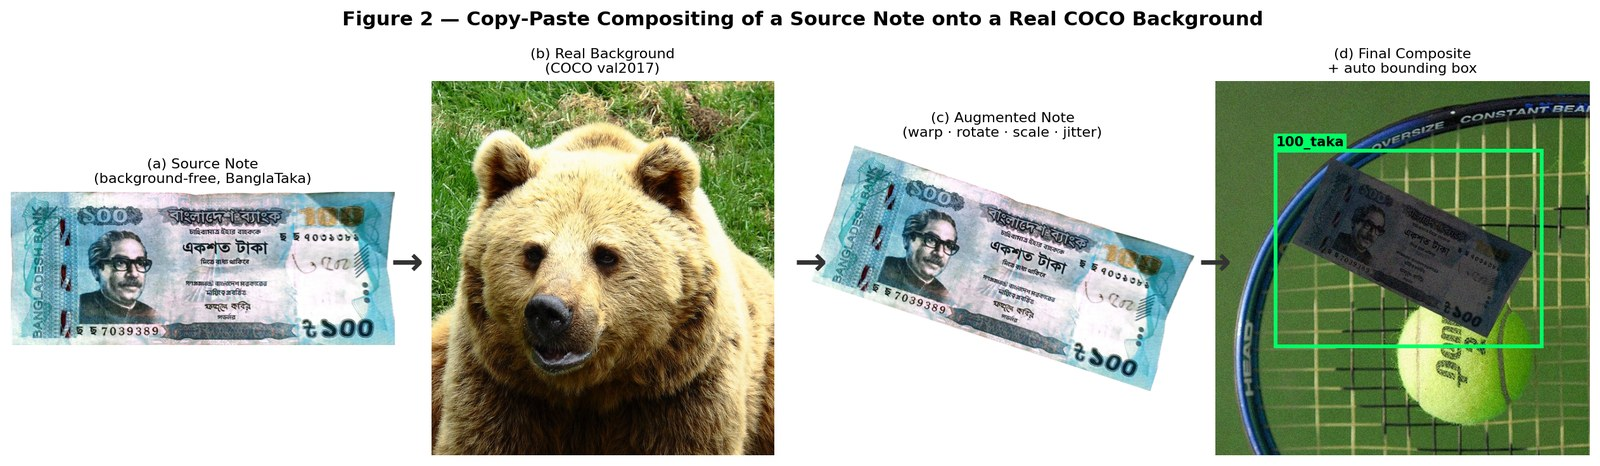
\includegraphics[width=0.9\textwidth]{fig_compositing.jpg}
    \caption{Copy-paste compositing applied to a 100 Taka note: (a) background-free source note, (b) real COCO background, (c) note after perspective warp, rotation, scaling and colour jitter, (d) final composite with the automatically generated bounding box and label}
    \label{fig:compositing}
\end{figure}

\subsection{Augmentation Operations}
Table~\ref{tab:aug} lists the domain-randomisation operations. The ranges were chosen to cover, and in most cases slightly exceed, the variation expected from a camera held by a person.

\begin{table}[!htbp]
\centering
\caption{Domain-randomisation operations used in compositing}
\label{tab:aug}
\begin{tabular}{|p{2.6cm}|p{4.6cm}|p{6cm}|}
\hline
\textbf{Stage} & \textbf{Operation} & \textbf{Setting} \\ \hline
\multirow{4}{*}{Geometry} & Perspective warp & 70\% probability, corner jitter 8\% \\ \cline{2-3}
 & Rotation & $\pm30^\circ$, expanded canvas, transparent fill \\ \cline{2-3}
 & Scale & Note occupies 0.25--0.90 of the canvas \\ \cline{2-3}
 & Placement & Random position \\ \hline
\multirow{2}{*}{Photometric} & HSV jitter & H $\pm18^\circ$, S $\times$0.5--1.5, V $\times$0.4--1.6 \\ \cline{2-3}
 & Brightness / contrast & 0.4--1.6 / 0.7--1.3 \\ \hline
\multirow{3}{*}{Sensor} & Motion blur & 20\% probability, kernel 3/5/7, horizontal or vertical \\ \cline{2-3}
 & Gaussian noise & 50\% probability, $\sigma \approx 12$ \\ \cline{2-3}
 & JPEG re-compression & Quality 55--92 \\ \hline
Balance & Negative images & 10\% background-only images with empty labels \\ \hline
\end{tabular}
\end{table}
\FloatBarrier

\subsection{Final Detection Dataset}
Four composites were generated per source note, plus background-only negatives. The data was split 80/10/10 \textit{by source note}, so no physical note image appears in more than one split (Table~\ref{tab:split}). The counts are those of the dataset as it is stored on disk; an earlier version of this thesis gave 22,315 images, a figure taken from a generation log that no longer matches the files.

\begin{table}[!htbp]
\centering
\caption{Composition of the synthetic Taka detection dataset}
\label{tab:split}
\begin{tabular}{|l|r|r|r|r|}
\hline
\textbf{Split} & \textbf{Positive} & \textbf{Negative} & \textbf{Total} & \textbf{Note instances} \\ \hline
Train & 16,224 & 1,615 & 17,839 & 16,224 \\ \hline
Validation & 2,016 & 196 & 2,212 & 2,016 \\ \hline
Test & 2,052 & 230 & 2,282 & 2,052 \\ \hline
\textbf{Total} & \textbf{20,292} & \textbf{2,041} & \textbf{22,333} & \textbf{20,292} \\ \hline
\end{tabular}
\end{table}

\subsection{Raw Photograph Test Set}
To test the detector on images that are not composites, 450 raw phone photographs of notes, 50 for each of the nine denominations, were taken from the raw BanglaTaka collection and labelled with their denomination. These images show real paper, real lighting and real camera noise, but they are not independent of the training data in the strict sense: the raw collection is the same source from which the training foregrounds were cropped, so some physical notes may overlap. This set is therefore a source-domain check, not a test.

\subsection{Independent Photograph Collections}
The real test of the detector uses photographs taken by other people and never used for training or selection. \textit{Bangla Money}, a public Kaggle collection, has 1,536 photographs of eight of the nine denominations (no 200 Taka) and 101 photographs of the 1 Taka note, a class the detector does not know. \textit{NSTU-BDTAKA} \cite{nstubdtaka2024} provides 186 annotated detection images and 1,144 close-ups in which a folded note is held in a hand. A third public collection was excluded because its files are byte-identical to the training source. A further set of 566 composites was built from the test-split notes on backgrounds from a different COCO subset, as a second synthetic test.

\section{Currency Authentication Data}
The authenticator is trained on the JaalTaka collection of genuine and counterfeit Bangladeshi notes \cite{jaaltaka}. Every physical note is photographed in six ordered close-up views that show different regions and security features (Figure~\ref{fig:jaaltaka}). Table~\ref{tab:jaaltaka} gives the statistics of the split used in all experiments.

\begin{figure}[H]
    \centering
    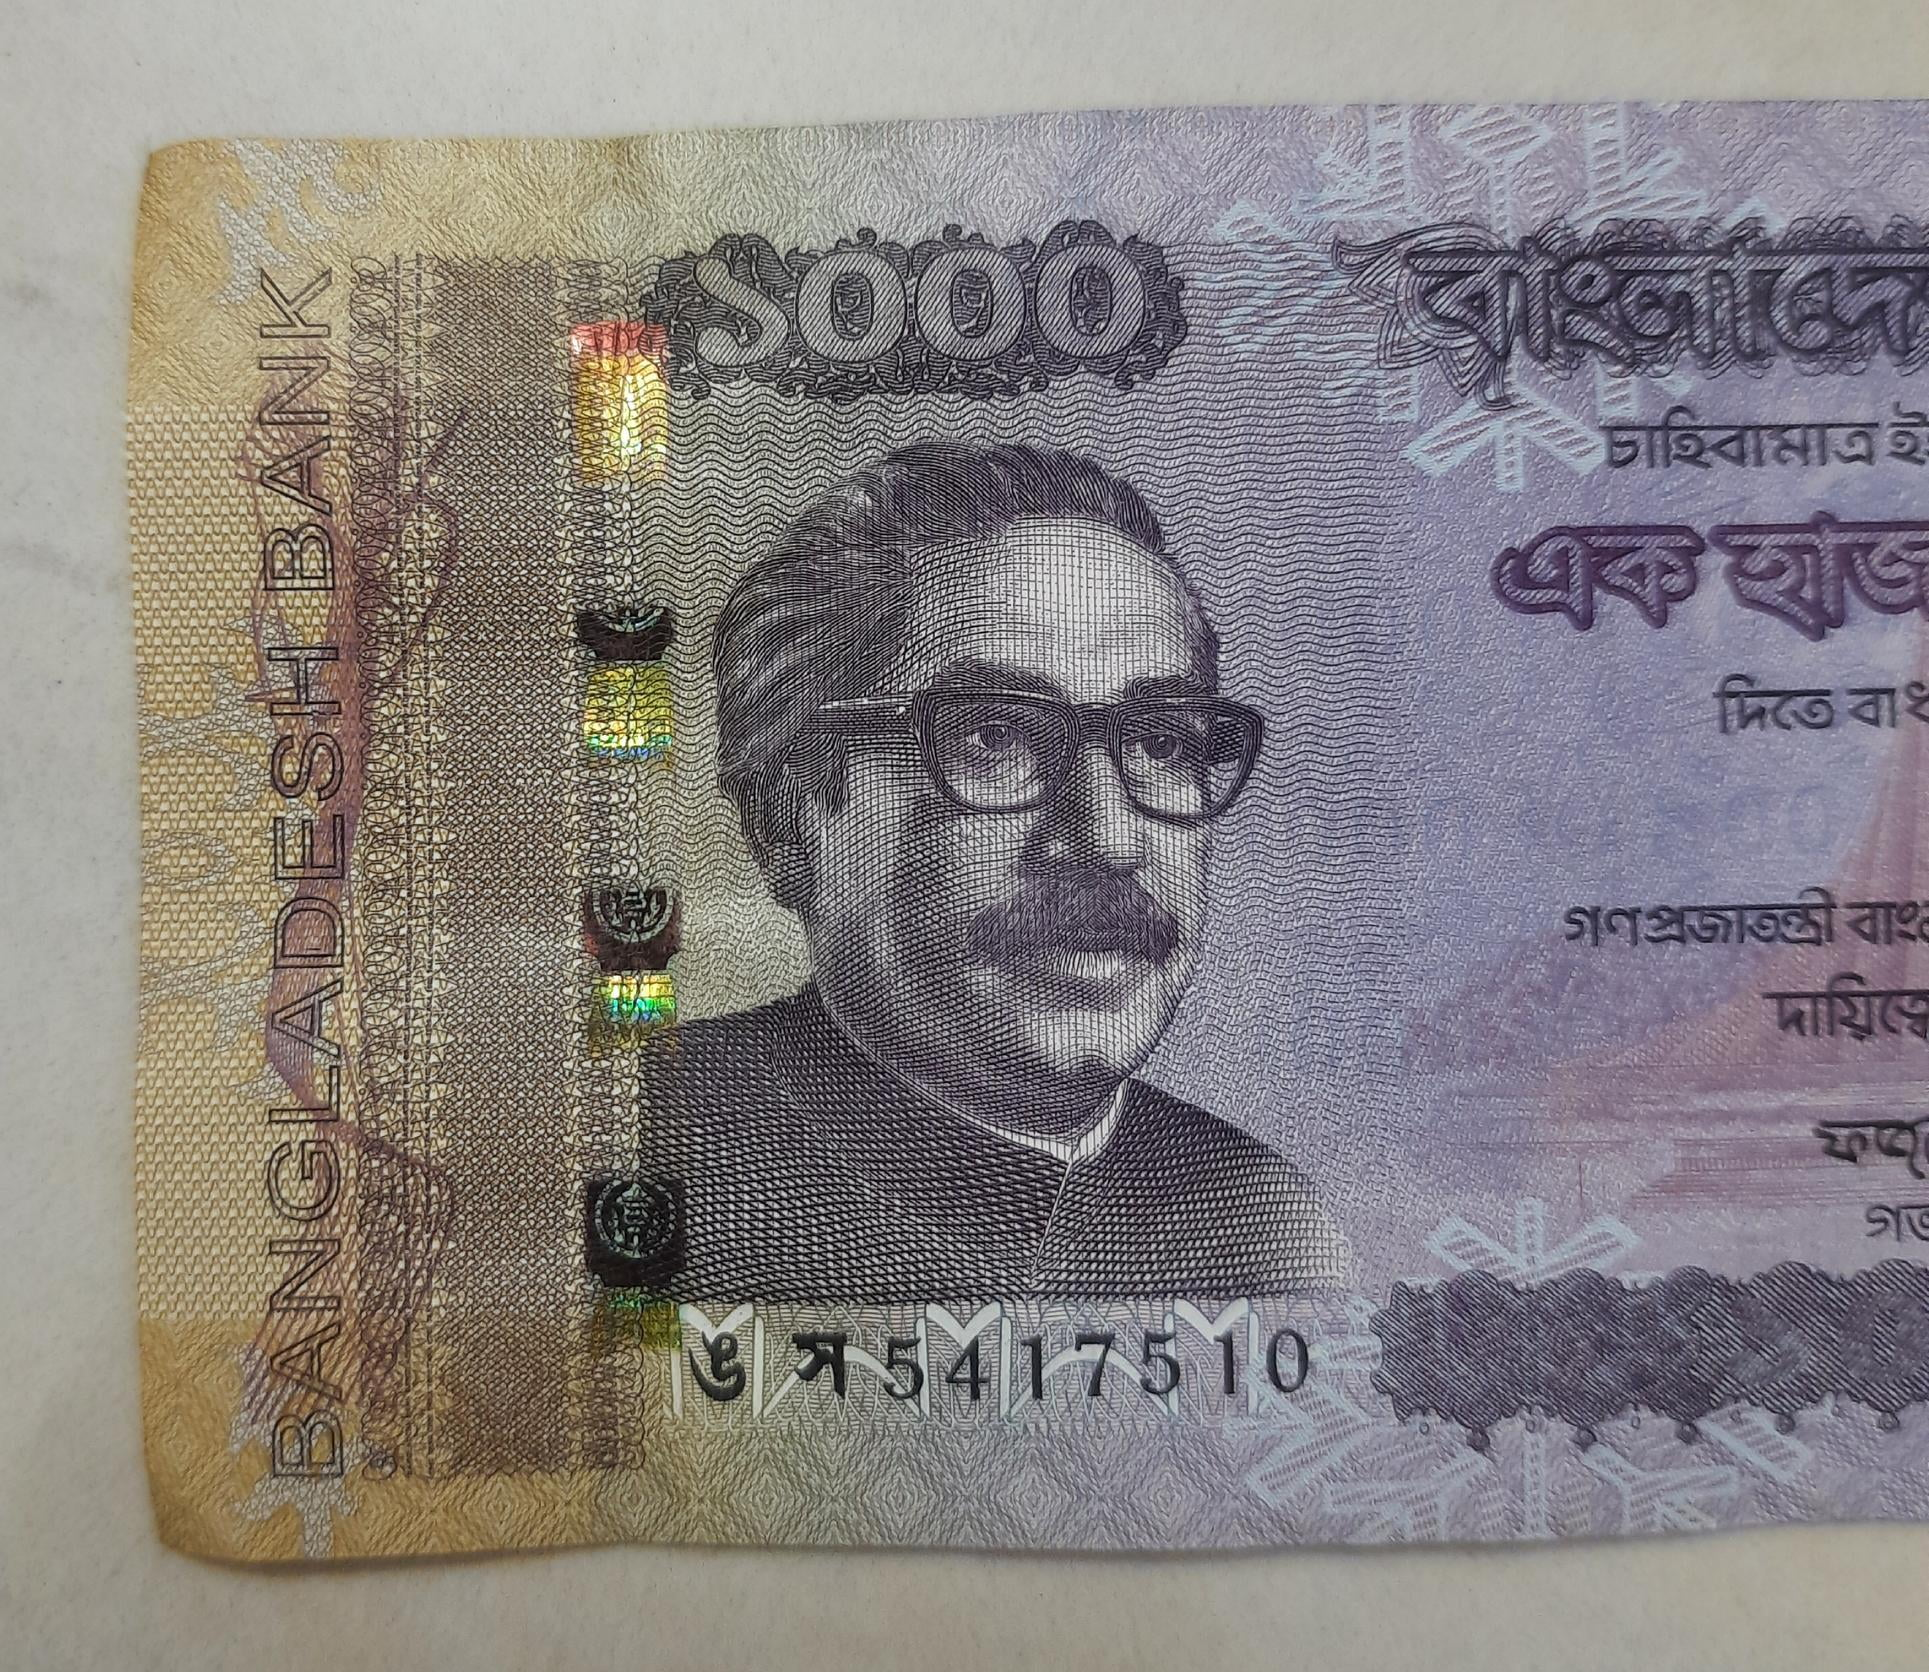
\includegraphics[width=0.3\textwidth]{jaal_real_v1.jpg}
    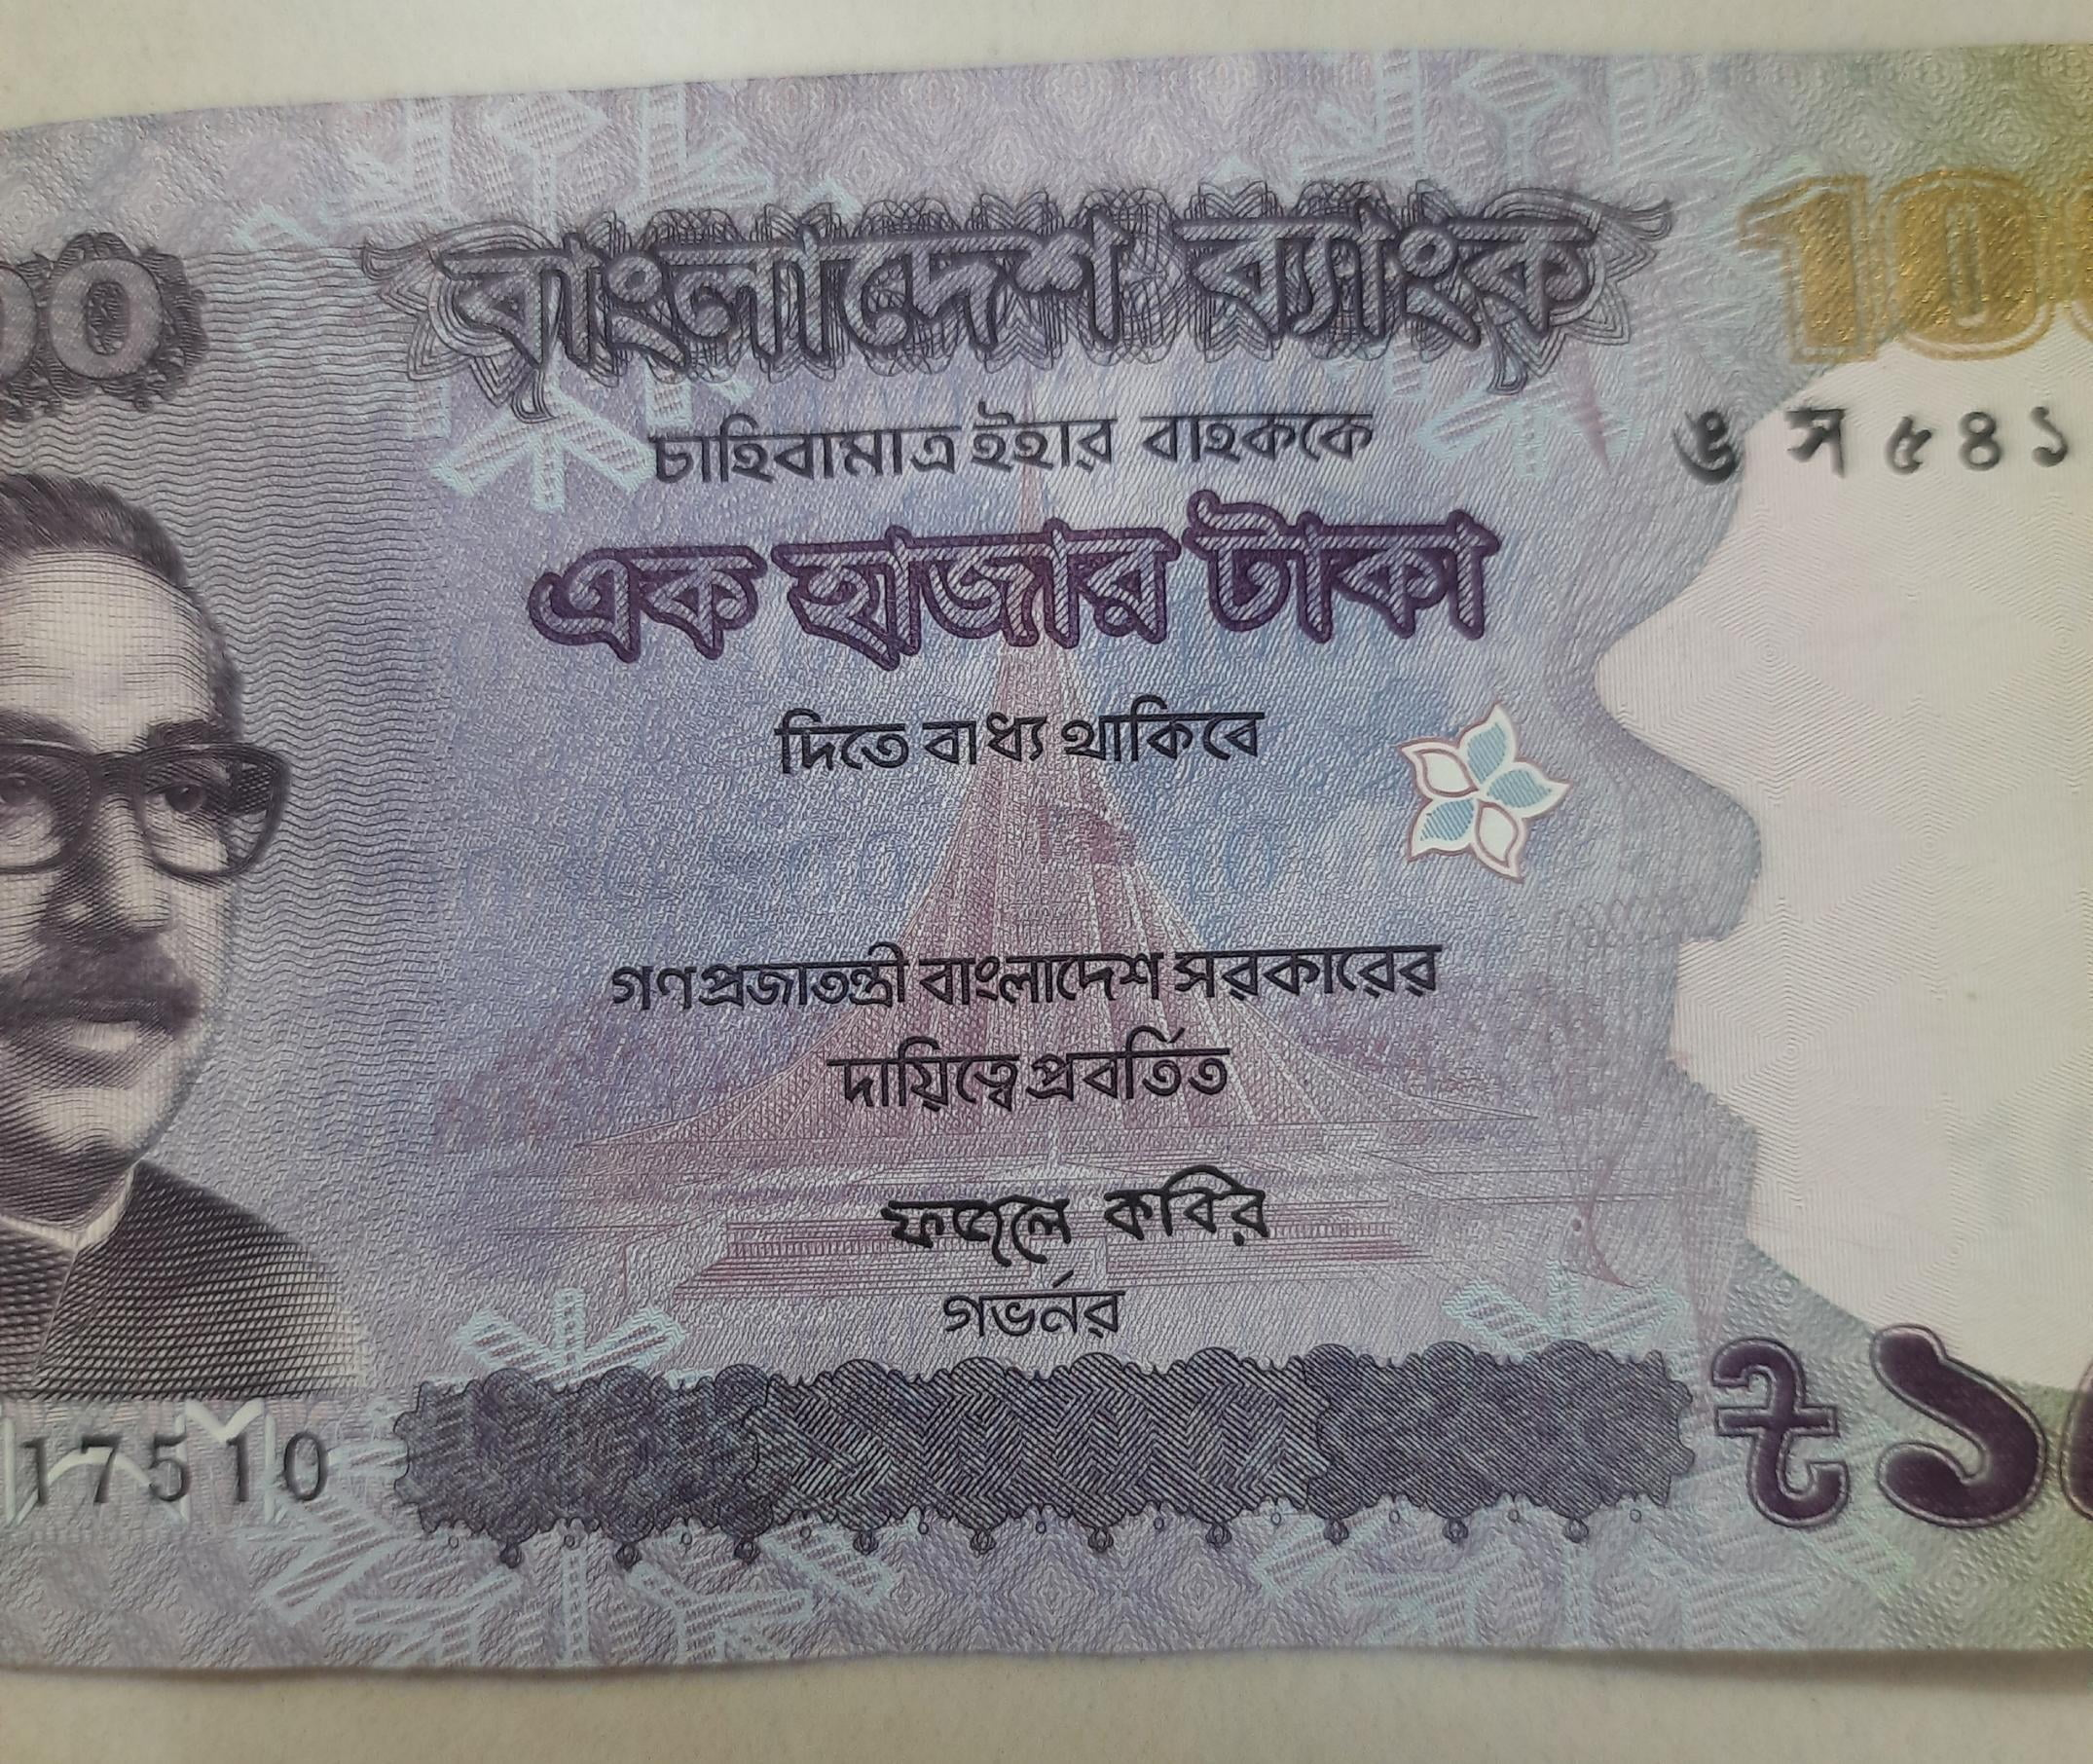
\includegraphics[width=0.3\textwidth]{jaal_real_v2.jpg}
    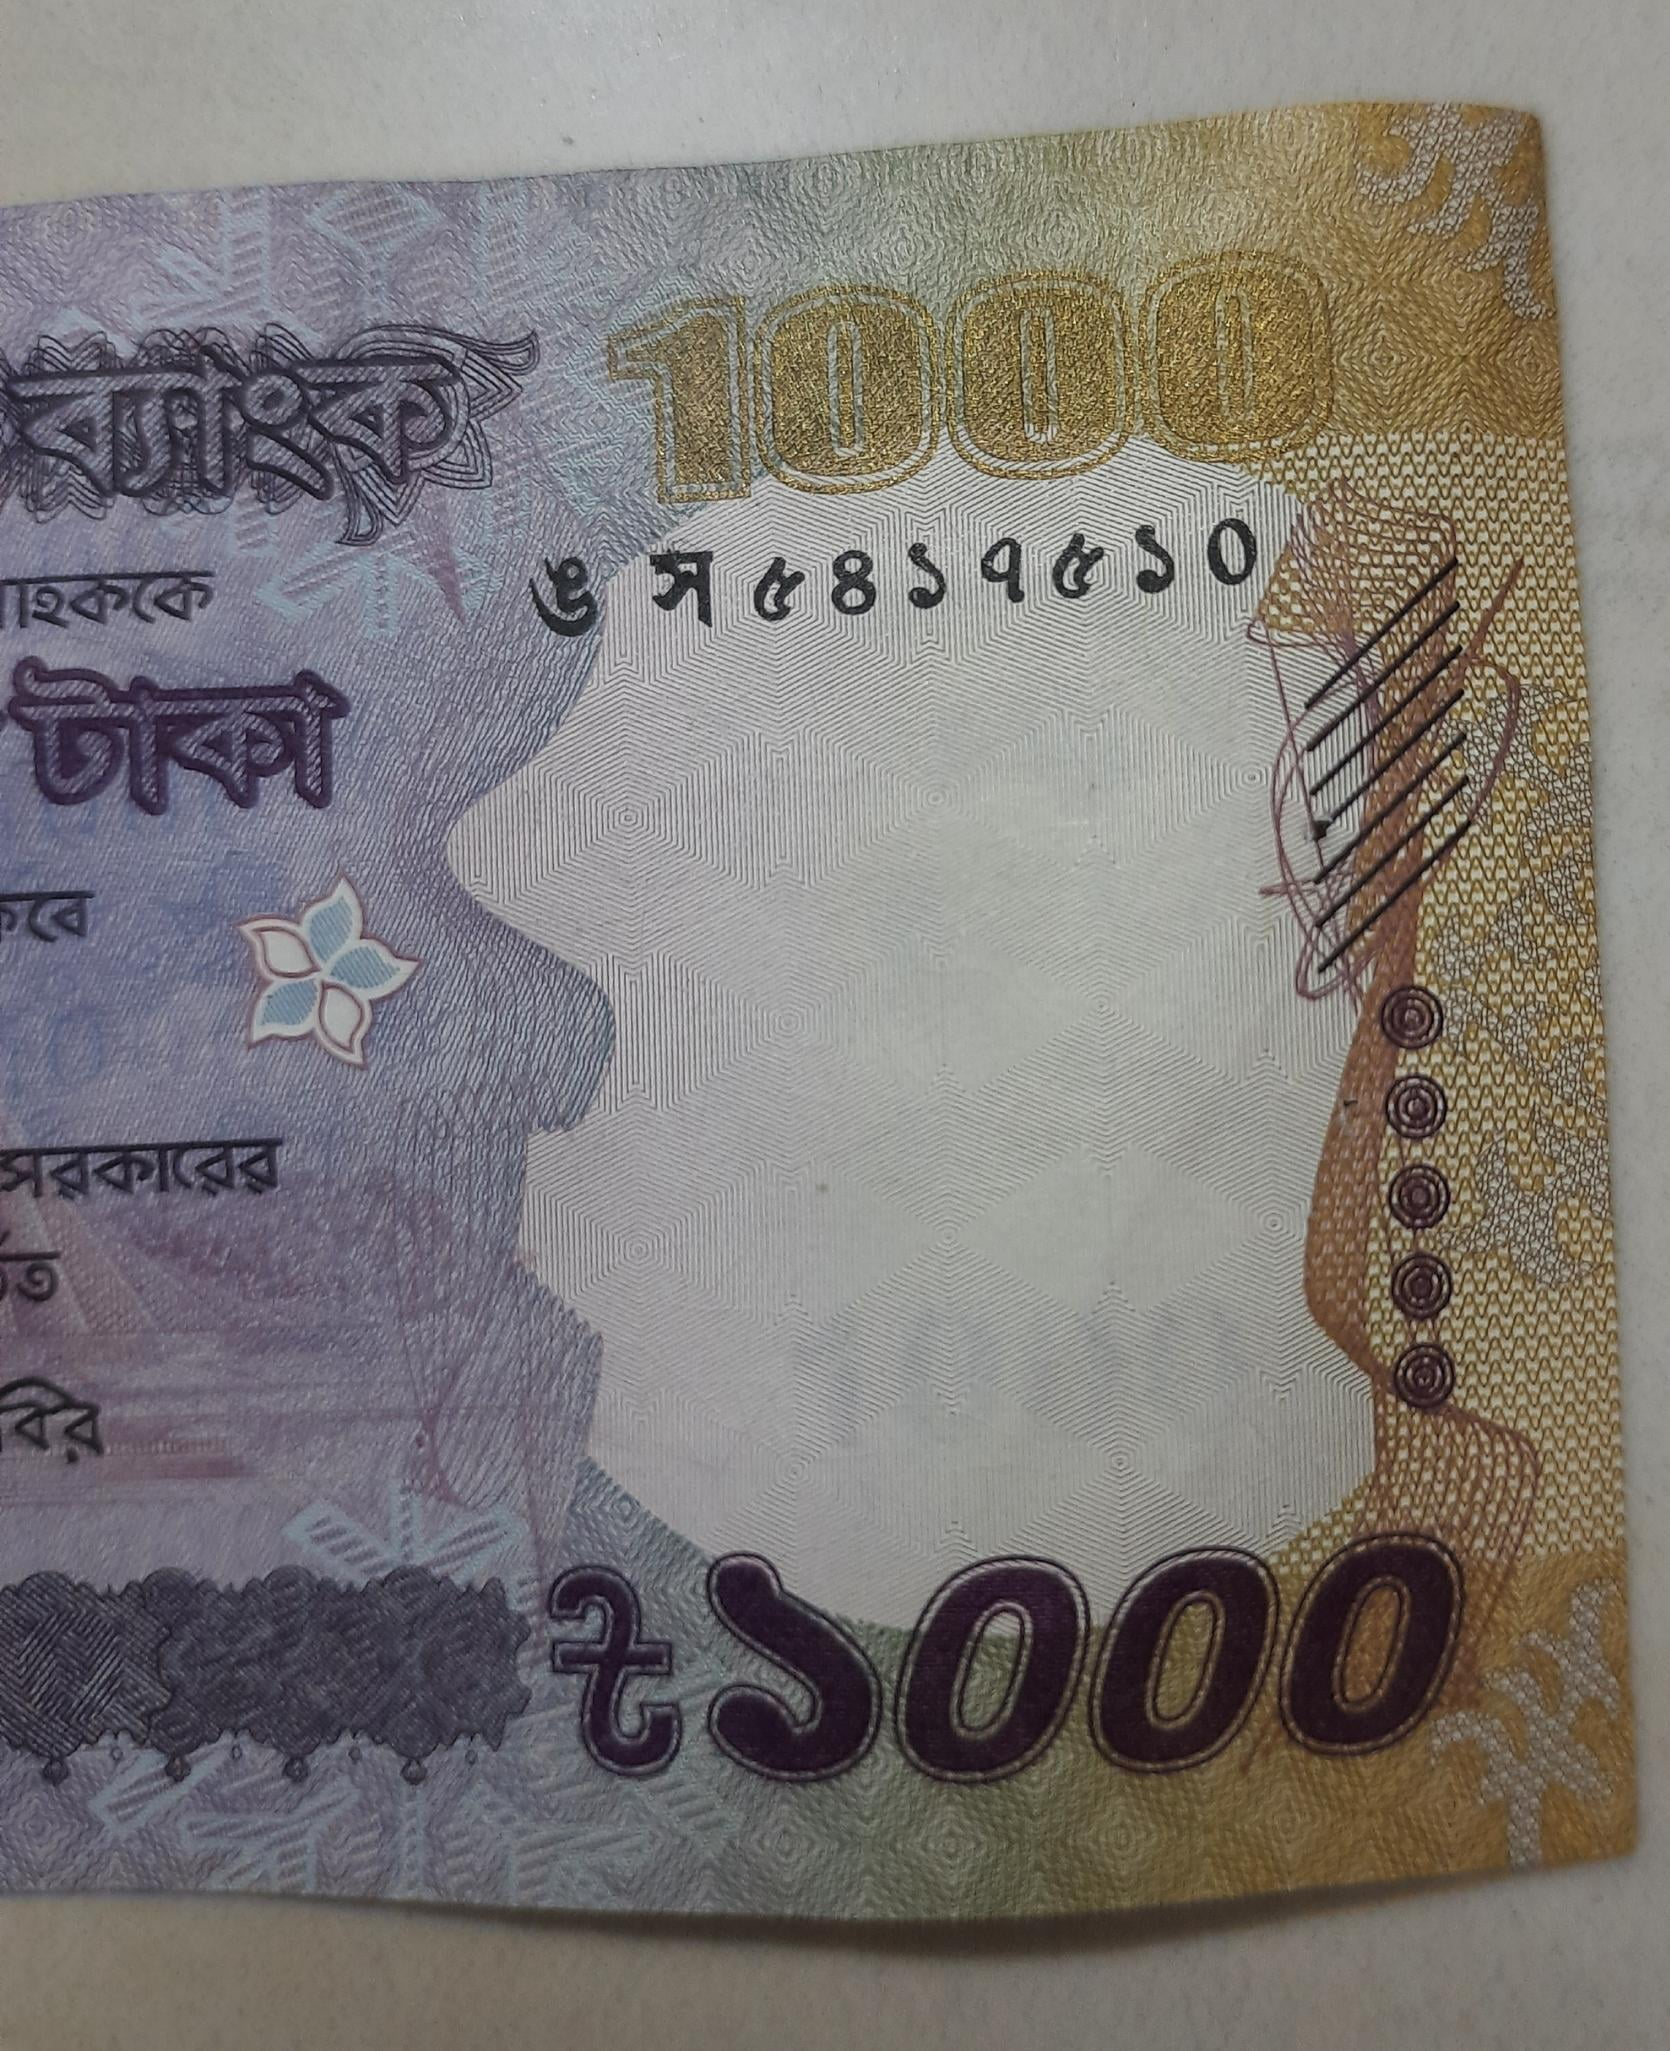
\includegraphics[width=0.3\textwidth]{jaal_real_v3.jpg}\\[3pt]
    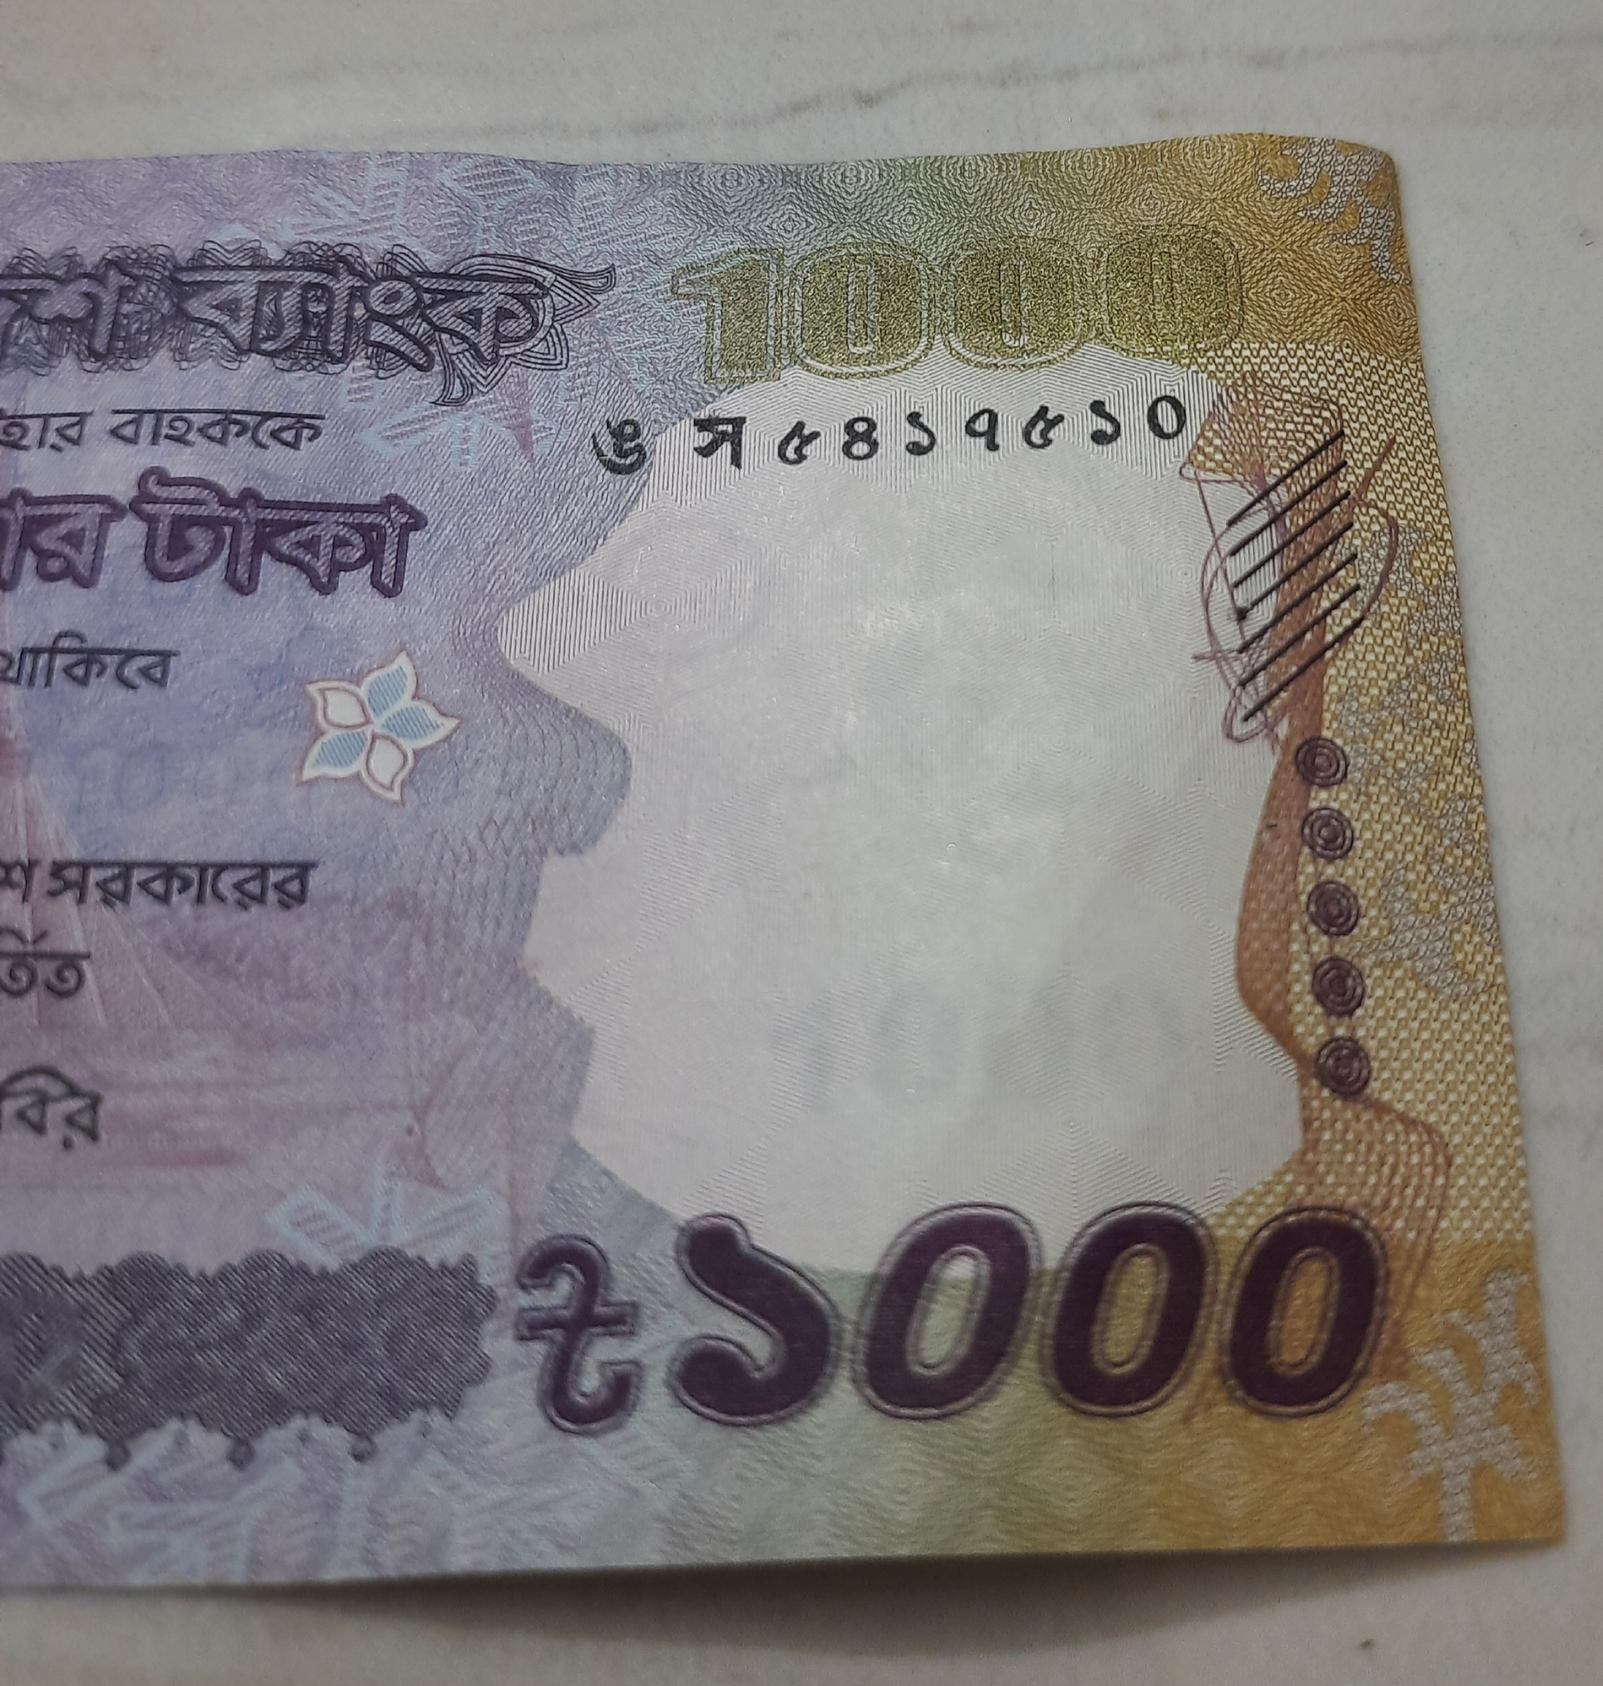
\includegraphics[width=0.3\textwidth]{jaal_real_v4.jpg}
    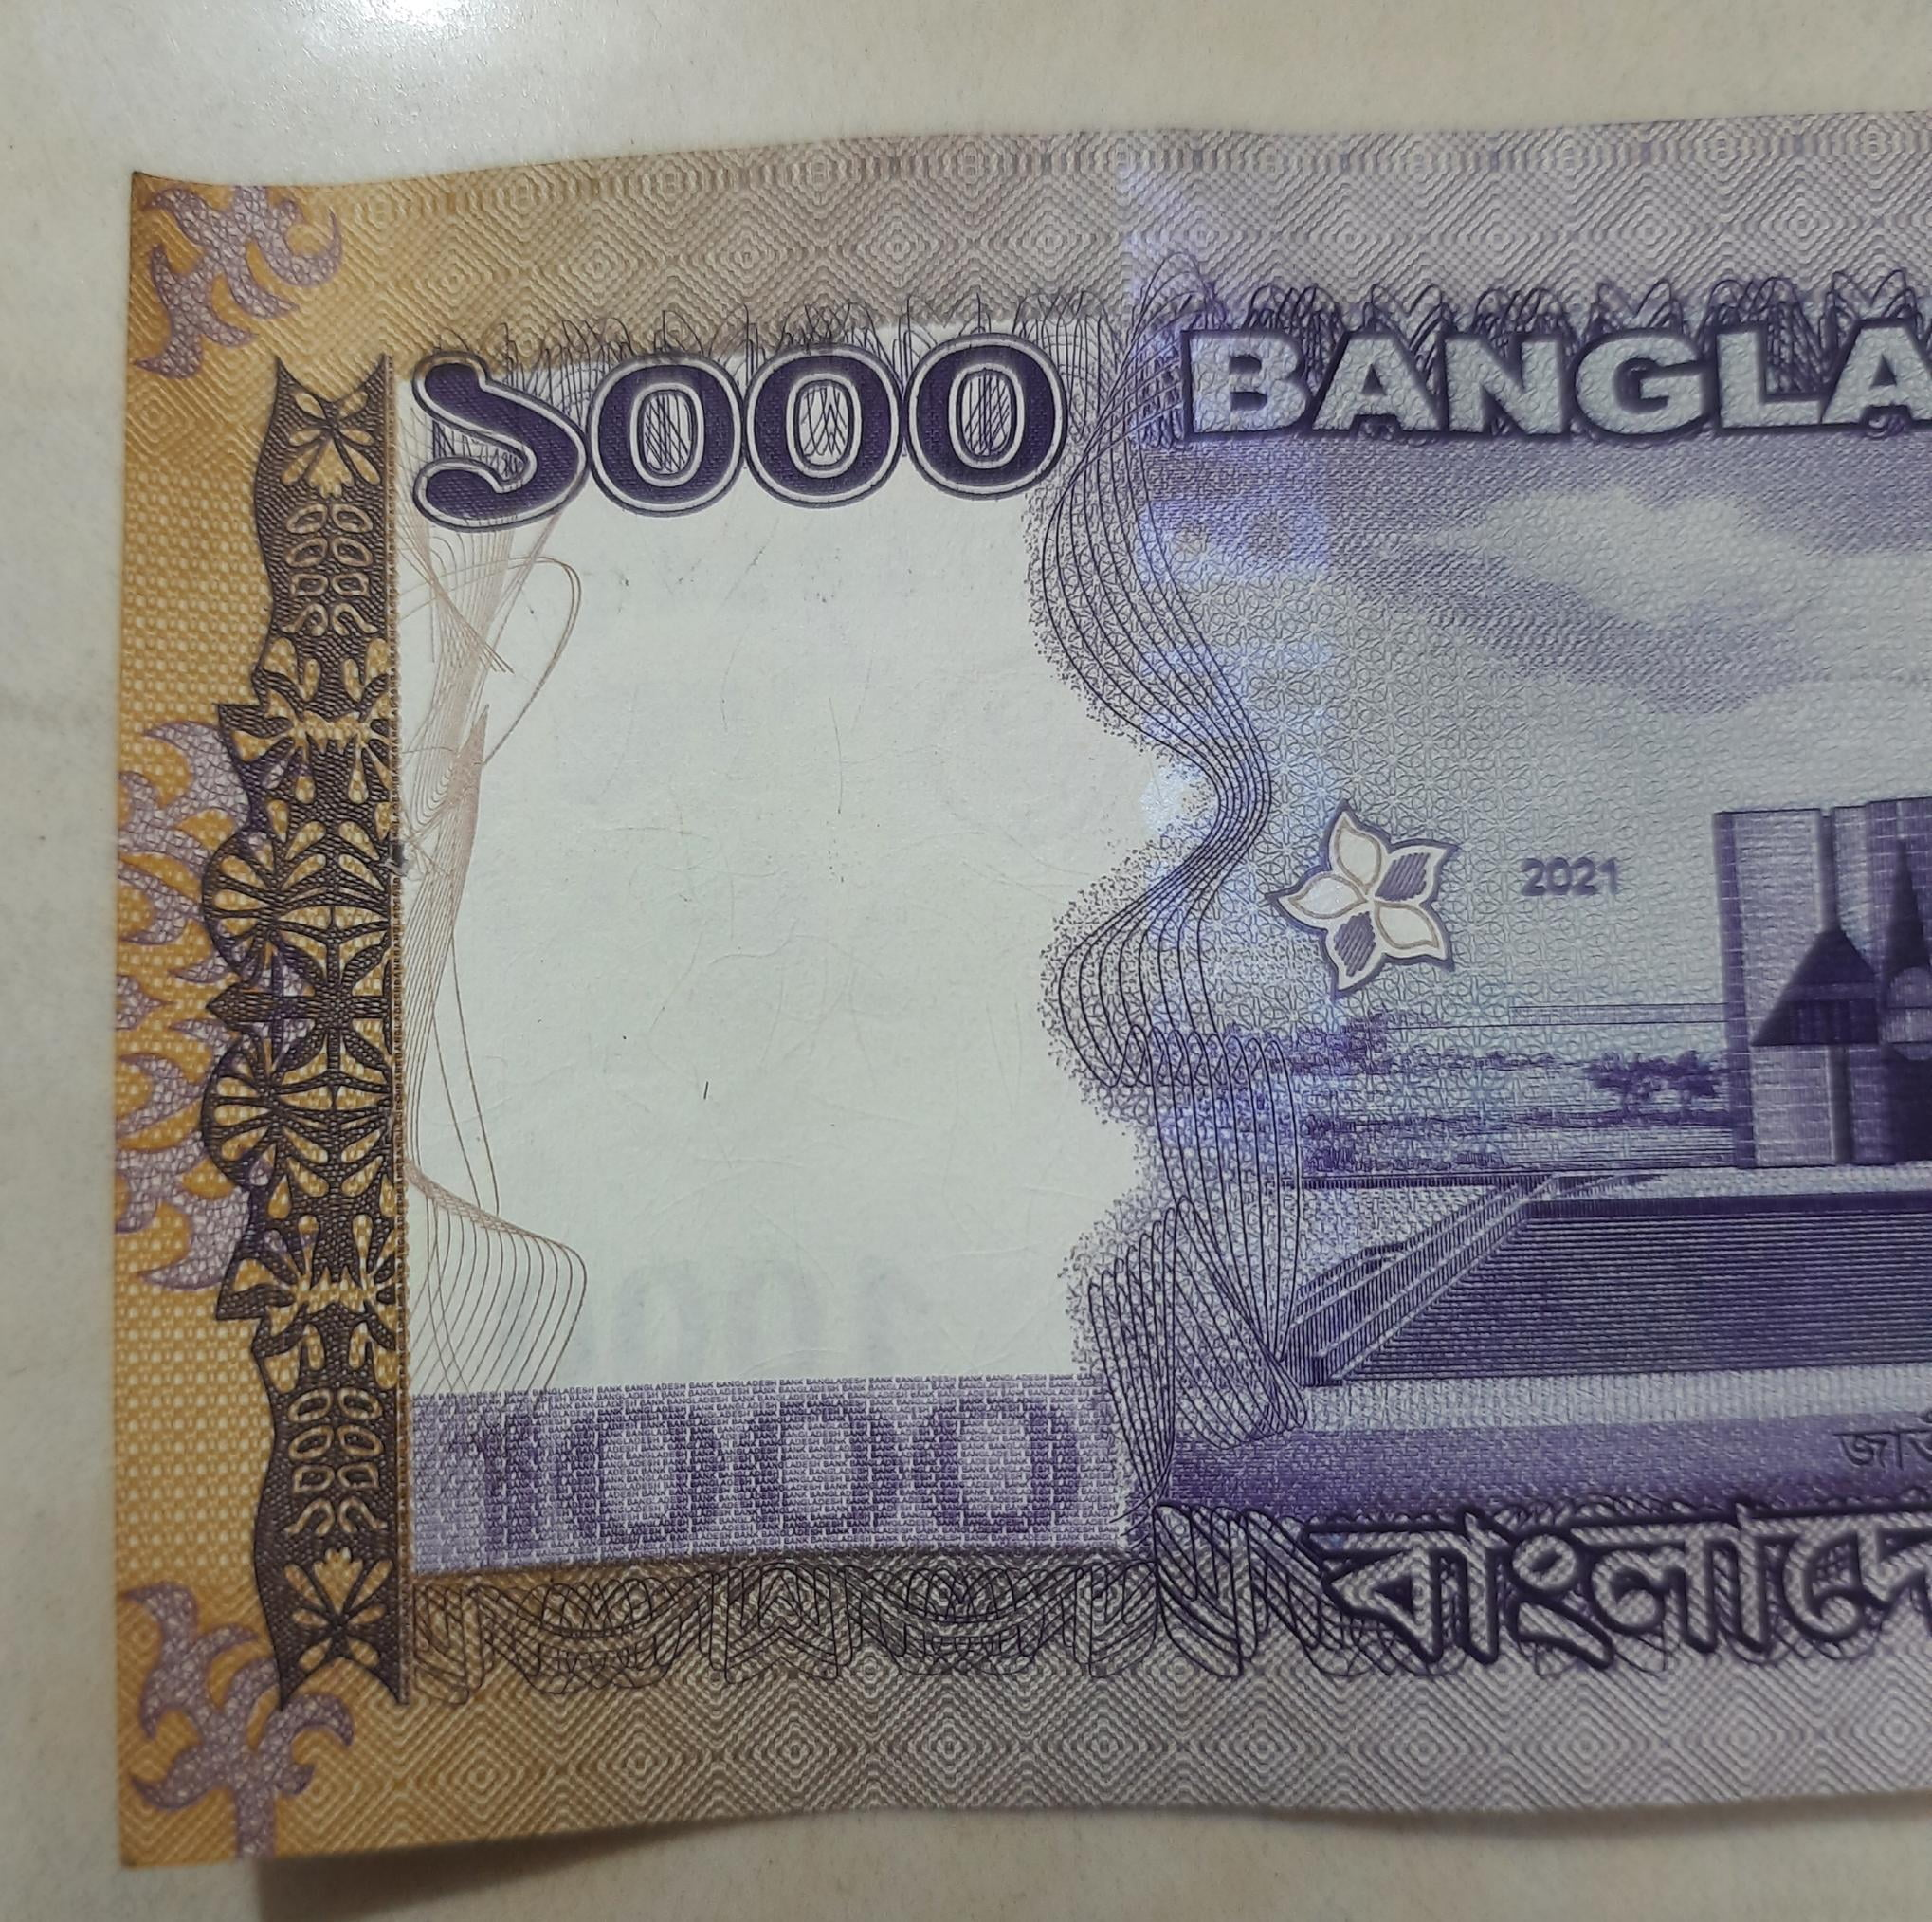
\includegraphics[width=0.3\textwidth]{jaal_real_v5.jpg}
    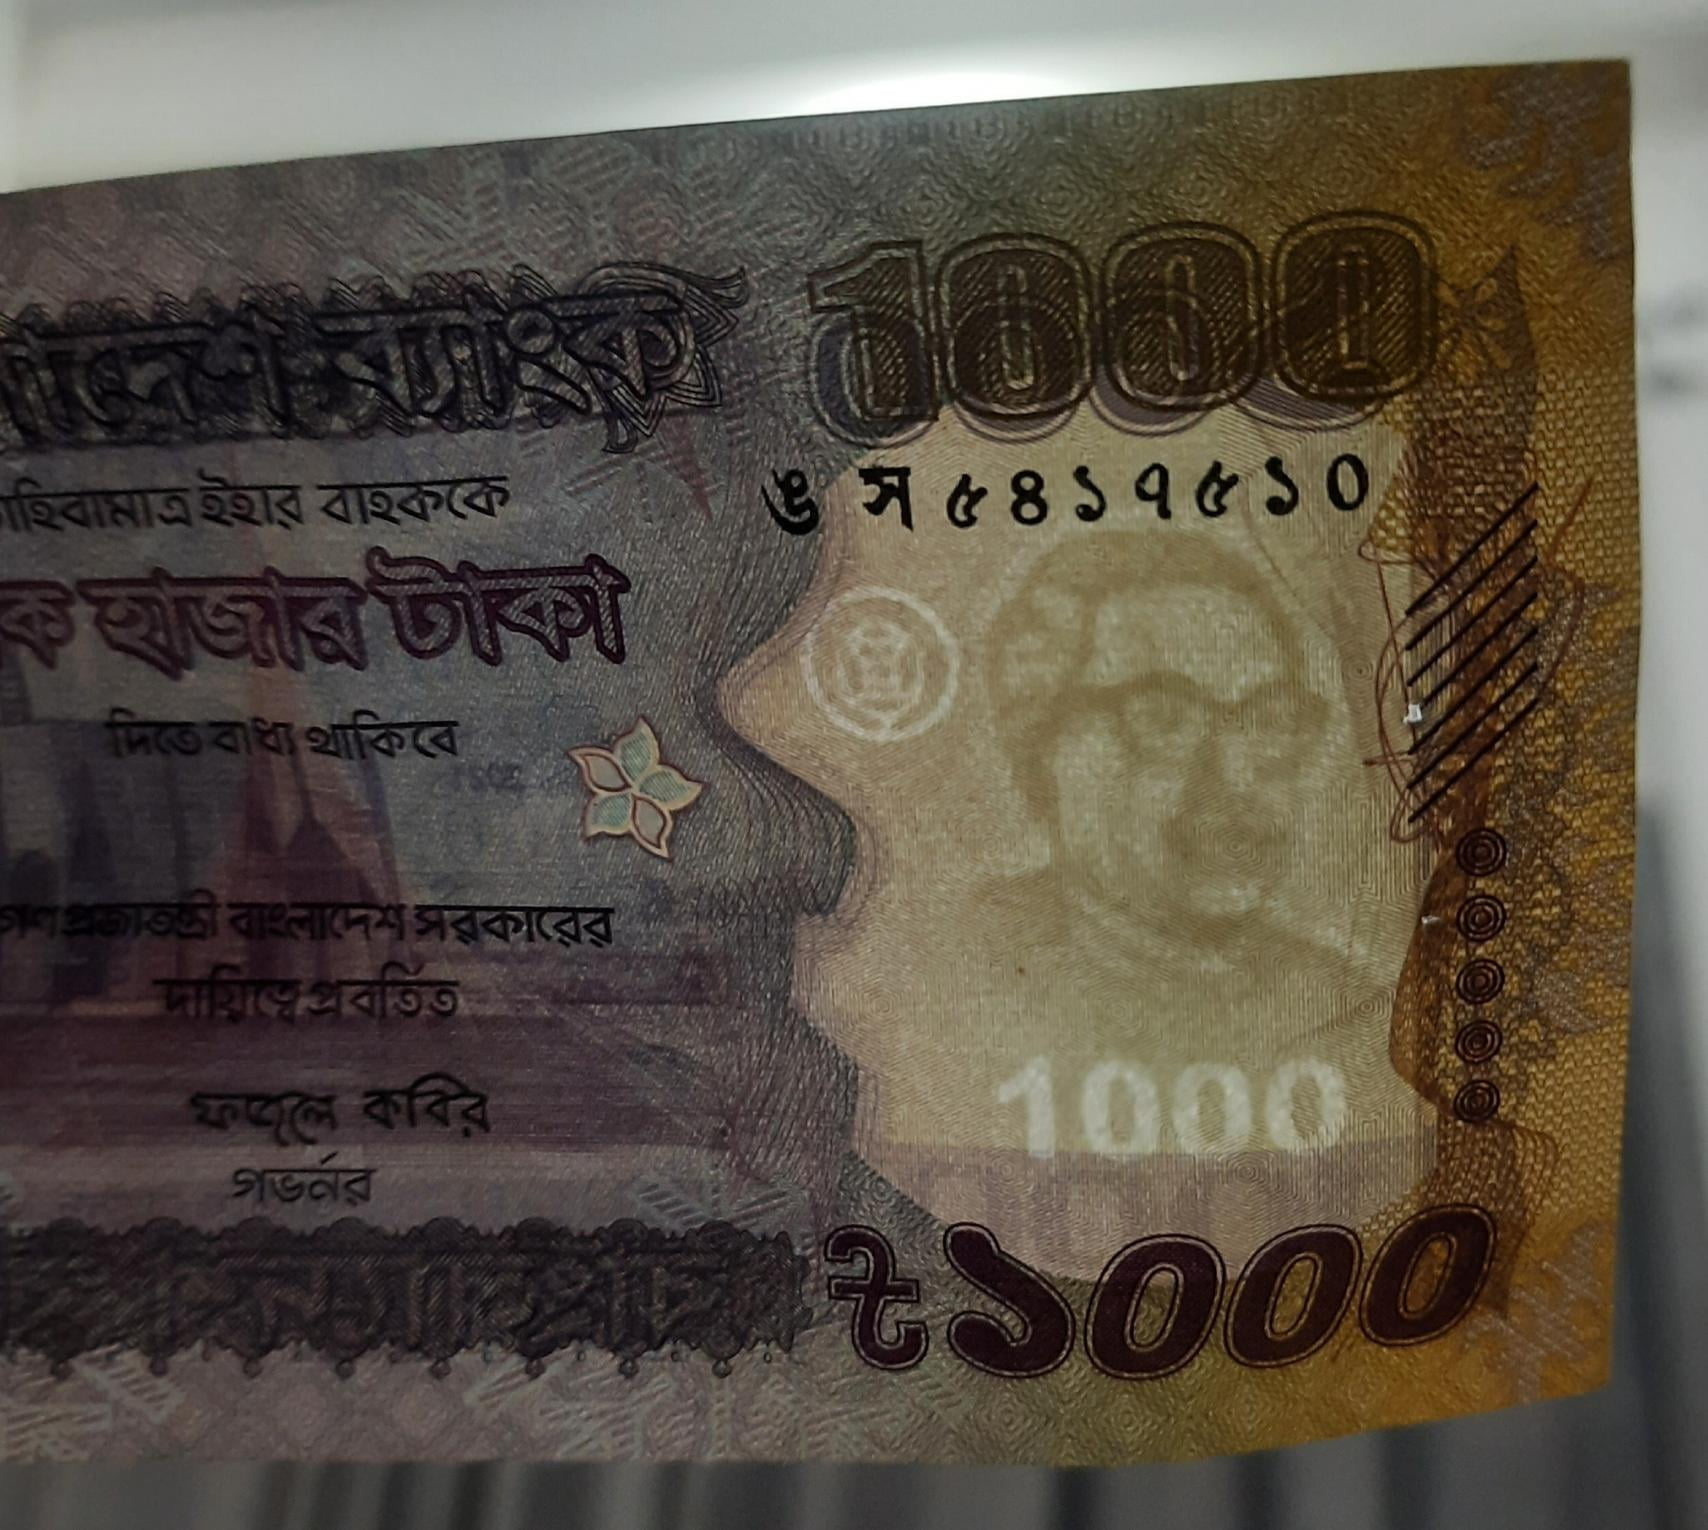
\includegraphics[width=0.3\textwidth]{jaal_real_v6.jpg}
    \caption{The six ordered views of one genuine note in the JaalTaka collection. Each view shows a different region, such as the portrait with the hologram strip and the serial number.}
    \label{fig:jaaltaka}
\end{figure}

\begin{table}[!htbp]
\centering
\caption{JaalTaka split used for authentication (split seed 42)}
\label{tab:jaaltaka}
\begin{tabular}{|l|c|}
\hline
\textbf{Item} & \textbf{Value} \\ \hline
Physical notes & 1,390 \\ \hline
Genuine / counterfeit notes & 802 / 588 \\ \hline
Views per note & 6 \\ \hline
Images & 8,340 \\ \hline
Train / validation / test notes & 974 / 208 / 208 \\ \hline
Train genuine / counterfeit & 562 / 412 \\ \hline
Note overlap between splits (train--val, train--test, val--test) & 0 / 0 / 0 \\ \hline
\end{tabular}
\end{table}

An earlier split of the same data at the image level produced an accuracy of 1.00, because views of the same note appeared in both training and test data. That number was a data-leakage artefact and is not reported as a result; all authentication results in this thesis use the note-disjoint split above or the print-disjoint split below.

\subsection{Serial-Number Audit}
\label{sec:serial_audit}
A genuine banknote has a unique serial number. A counterfeit is printed from a scanned or engraved original, so every copy of one print carries the same serial. To see how many distinct prints JaalTaka contains, the serial number at the lower left of each note was read with OCR, Bangla digits were mapped to 0--9, and the first six digits were compared (one digit can be misread). Table~\ref{tab:serial} gives the result.

\begin{table}[!htbp]
\centering
\caption{Serial numbers read from JaalTaka notes}
\label{tab:serial}
\begin{tabular}{|l|c|c|c|p{4.6cm}|}
\hline
\textbf{Class} & \textbf{Notes} & \textbf{Serial read} & \textbf{Distinct} & \textbf{Most common serial} \\ \hline
500 Taka counterfeit & 324 & 322 & 27 & on 279 notes (86.6\% of those read) \\ \hline
1,000 Taka counterfeit & 261 & 201 & 66 & on 43 notes; two near-identical readings on 29 more \\ \hline
500 Taka genuine & 397 & 331 & 233 & 1.2\% \\ \hline
1,000 Taka genuine & 401 & 270 & 227 & 1.5\% \\ \hline
\end{tabular}
\end{table}

Genuine notes have almost one serial per note. Counterfeit notes are dominated by a few serials: 279 of the 322 readable 500 Taka counterfeits carry the same one. The note-disjoint split is therefore not print-disjoint. On its test split, 68 of 87 counterfeits have a serial that also occurs on a training counterfeit, and a rule that needs no knowledge of counterfeiting at all, ``counterfeit if the serial occurs among the training counterfeits'', scores 90.2\% on the 205 test notes that could be reconstructed as whole notes. This is a shortcut in the sense of \cite{geirhos2020shortcut}, and it affects every result published on this split, not only ours. The data article does not mention it.

\subsection{Print-Disjoint Split}
\label{sec:serial_split}
A second split was built in which no test counterfeit shares its serial with a training or validation counterfeit: 946 training, 222 validation and 222 test notes. The test split has 121 genuine and 101 counterfeit notes, and its counterfeits come from about 24 distinct prints. This small number is the real size of the test: two detectors can only be compared on about 24 independent counterfeit prints, however many notes there are. All results labelled ``unseen prints'' in Chapter~\ref{chap:results} use this split.

\subsection{Back-Lit Views and Watermark Labels}
The sixth view of each note is a back-lit photograph in which the watermark is visible on a genuine note. For the watermark classifier, the window was cut from each back-lit view after registration to a note template; registration succeeded on 867 of 946 training, 197 of 222 validation and 197 of 222 test photographs. The corner positions of these windows, mapped back into each photograph, are the training labels of the localizer.

\subsection{Whole-Note Counterfeit Photographs}
The glass sees whole notes, not close-up views. To check the deployed verdict, the Bangladeshi Counterfeit Currency Image Dataset was used, which has whole-note photographs of 500 and 1,000 Taka notes: 1,199 genuine and 87 counterfeit, of which 60 are augmented copies. The counterfeit photographs show about four physical notes, so this set can support a safety check but cannot prove it. The genuine 500 and 1,000 Taka photographs of Bangla Money and BanglaTaka were used as further genuine notes.

\subsection{A Tool for a Larger Print-Disjoint Dataset}
A dataset with about 100 unseen counterfeit prints would be needed to compare detectors with confidence. Such notes can only be obtained with a bank or the police, which was outside the reach of this project. A collection tool was written for that future work: it registers each photograph with its note and its print, refuses a print that would appear in two splits, a note that changes print, contradicting labels and duplicates, and exports the split. A second tool records the watermark window by four mouse clicks, and the localizer training script accepts these labels.

\section{Emotion Recognition Data}
Emotion recognition uses the Real-world Affective Faces Database (RAF-DB) \cite{rafdb} with its official training (12,271 images) and test (3,068 images) split. The class distribution of the test set is imbalanced (Table~\ref{tab:rafdb}): happy faces are sixteen times as frequent as fearful ones, which later explains the weaker recall for fear and disgust.

\begin{table}[!htbp]
\centering
\caption{Class distribution of the RAF-DB official test set}
\label{tab:rafdb}
\begin{tabular}{|l|c|c|c|c|c|c|c|c|}
\hline
\textbf{Class} & Happy & Sad & Angry & Surprise & Fear & Disgust & Neutral & \textbf{Total} \\ \hline
\textbf{Images} & 1,185 & 478 & 162 & 329 & 74 & 160 & 680 & \textbf{3,068} \\ \hline
\end{tabular}
\end{table}

\section{Text Recognition Data}
\subsection{OCR Benchmark}
\label{sec:ocr_bench_data}
The first OCR test set of this project had 80 phrases rendered with one font. Two faults made its numbers unusable. First, the images were drawn with a graphics library that, on the development machine, did not shape Bangla text: vowel signs that belong before the consonant were drawn after it, and conjuncts were broken apart. Real print never looks like that. Second, the correction step of the OCR mode used a word list that contained the test phrases. A new benchmark was therefore built:
\begin{itemize}[noitemsep]
    \item \textbf{Shaping.} Text is shaped with HarfBuzz \cite{harfbuzz} and drawn with FreeType, the way a printer or a browser does it.
    \item \textbf{Phrases.} Short phrases of the kind a visually impaired person needs to read (signs, counters, labels, directions). The validation set has 24 Bangla and 24 English phrases; the test set has 48 other phrases. A further 24 phrases were used once, for the canvas-size decision.
    \item \textbf{Fonts.} Validation images use Nirmala UI and Noto Serif Bengali for Bangla and Georgia and Verdana for English; test images use Nirmala UI, Noto Sans Bengali and Tiro Bangla, and Arial, Times and Calibri. In all, 10 Bangla and 9 Latin fonts are used, and the fonts used to train a recogniser are never scored.
    \item \textbf{Conditions.} Every phrase appears three ways: on a clean page, on a distorted page (rotation, blur, low resolution), and as a sign placed into a real COCO photograph at 640$\times$480 pixels, the frame size of the glass.
    \item \textbf{Seeds.} Three image seeds, giving 432 images per phrase set.
\end{itemize}
Every choice was made on the validation set; the test set was read once per finished method. For the fine-tuning experiment, training text came from general frequency lists of 50,000 Bangla and 50,000 English words, with every word of every benchmark phrase removed.

\subsection{Ekush Handwritten Characters}
As an additional study of Bangla recognition, a CNN classifier for 122 classes of isolated handwritten Bangla characters (vowels, consonants, conjuncts, modifiers and digits) was trained on the Ekush dataset \cite{ekush}. The data was split by writer (2,429 / 303 / 305 writers; 292,974 / 35,436 / 38,608 images) so that no writer's handwriting appears in both training and test data.

\section{Object Detection Data}
The object mode uses a YOLOv8 model pre-trained on COCO without retraining. To check its accuracy in our pipeline, it was evaluated on a random subset of 250 images from COCO val2017, in which 77 of the 80 classes appear.

\section{Note on User Survey}
This work does not yet include results from a study with visually impaired participants. Trial sessions and a survey have started (Section~\ref{sec:field_test}), and their data will be added when they are complete. A protocol has been prepared and its hypotheses and analysis were written down in advance (8--12 participants; tasks for denomination identification, the watermark check with and without spoken guidance, and reading; measures including task time, accuracy, NASA-TLX \cite{nasatlx} and the System Usability Scale \cite{sus}). The software for it exists: the study log of the watermark check, an analysis script, and the voice-driven questionnaire. The questionnaire tool was tried in three pilot sessions run by the project team, each about three and a half minutes long, to test that names and spoken answers are recorded; in the last two sessions five and six of the six answers were recognised from speech. These sessions test the tool. They are not study data, and no user-study result is reported in this thesis. Conducting the study, with ethical approval, is the most important next step (Chapter~\ref{chap:conclusion}).

\clearpage
\chapter{Result and Discussion}
\label{chap:results}

\section{Performance Evaluation Overview}

The evaluation of Savior Glass covers six functional areas: Taka detection, Taka authentication, emotion recognition, text recognition, object detection and processing speed. Each module was evaluated on held-out data that was not used for training or model selection, using the protocol described in Section~\ref{sec:method}. Model training and evaluation were run on laptop GPUs (NVIDIA RTX~4060 for the Taka detector, RTX~3050 for the other models); speed on the laptop CPU is also reported. Every number in this chapter was copied from a saved evaluation file of the project. When a measurement does not exist, it is written as \textit{not measured} rather than estimated.

\section{Taka Detection Performance}

\subsection{Training Behaviour}
The YOLOv8s detector was fine-tuned from COCO weights for 80 epochs at 640$\times$640 pixels with batch size 16, SGD (initial learning rate 0.01, momentum 0.937, weight decay 0.0005, three warm-up epochs), mosaic 1.0 and mixup 0.15. Horizontal and vertical flips were disabled because a mirrored note is not a real note. Training converged quickly: mAP@0.5 was above 0.97 after 8 epochs and above 0.99 after 11 epochs, while mAP@0.5:0.95 kept improving slowly as the boxes became tighter (Figure~\ref{fig:traincurves}).

\begin{figure}[H]
    \centering
    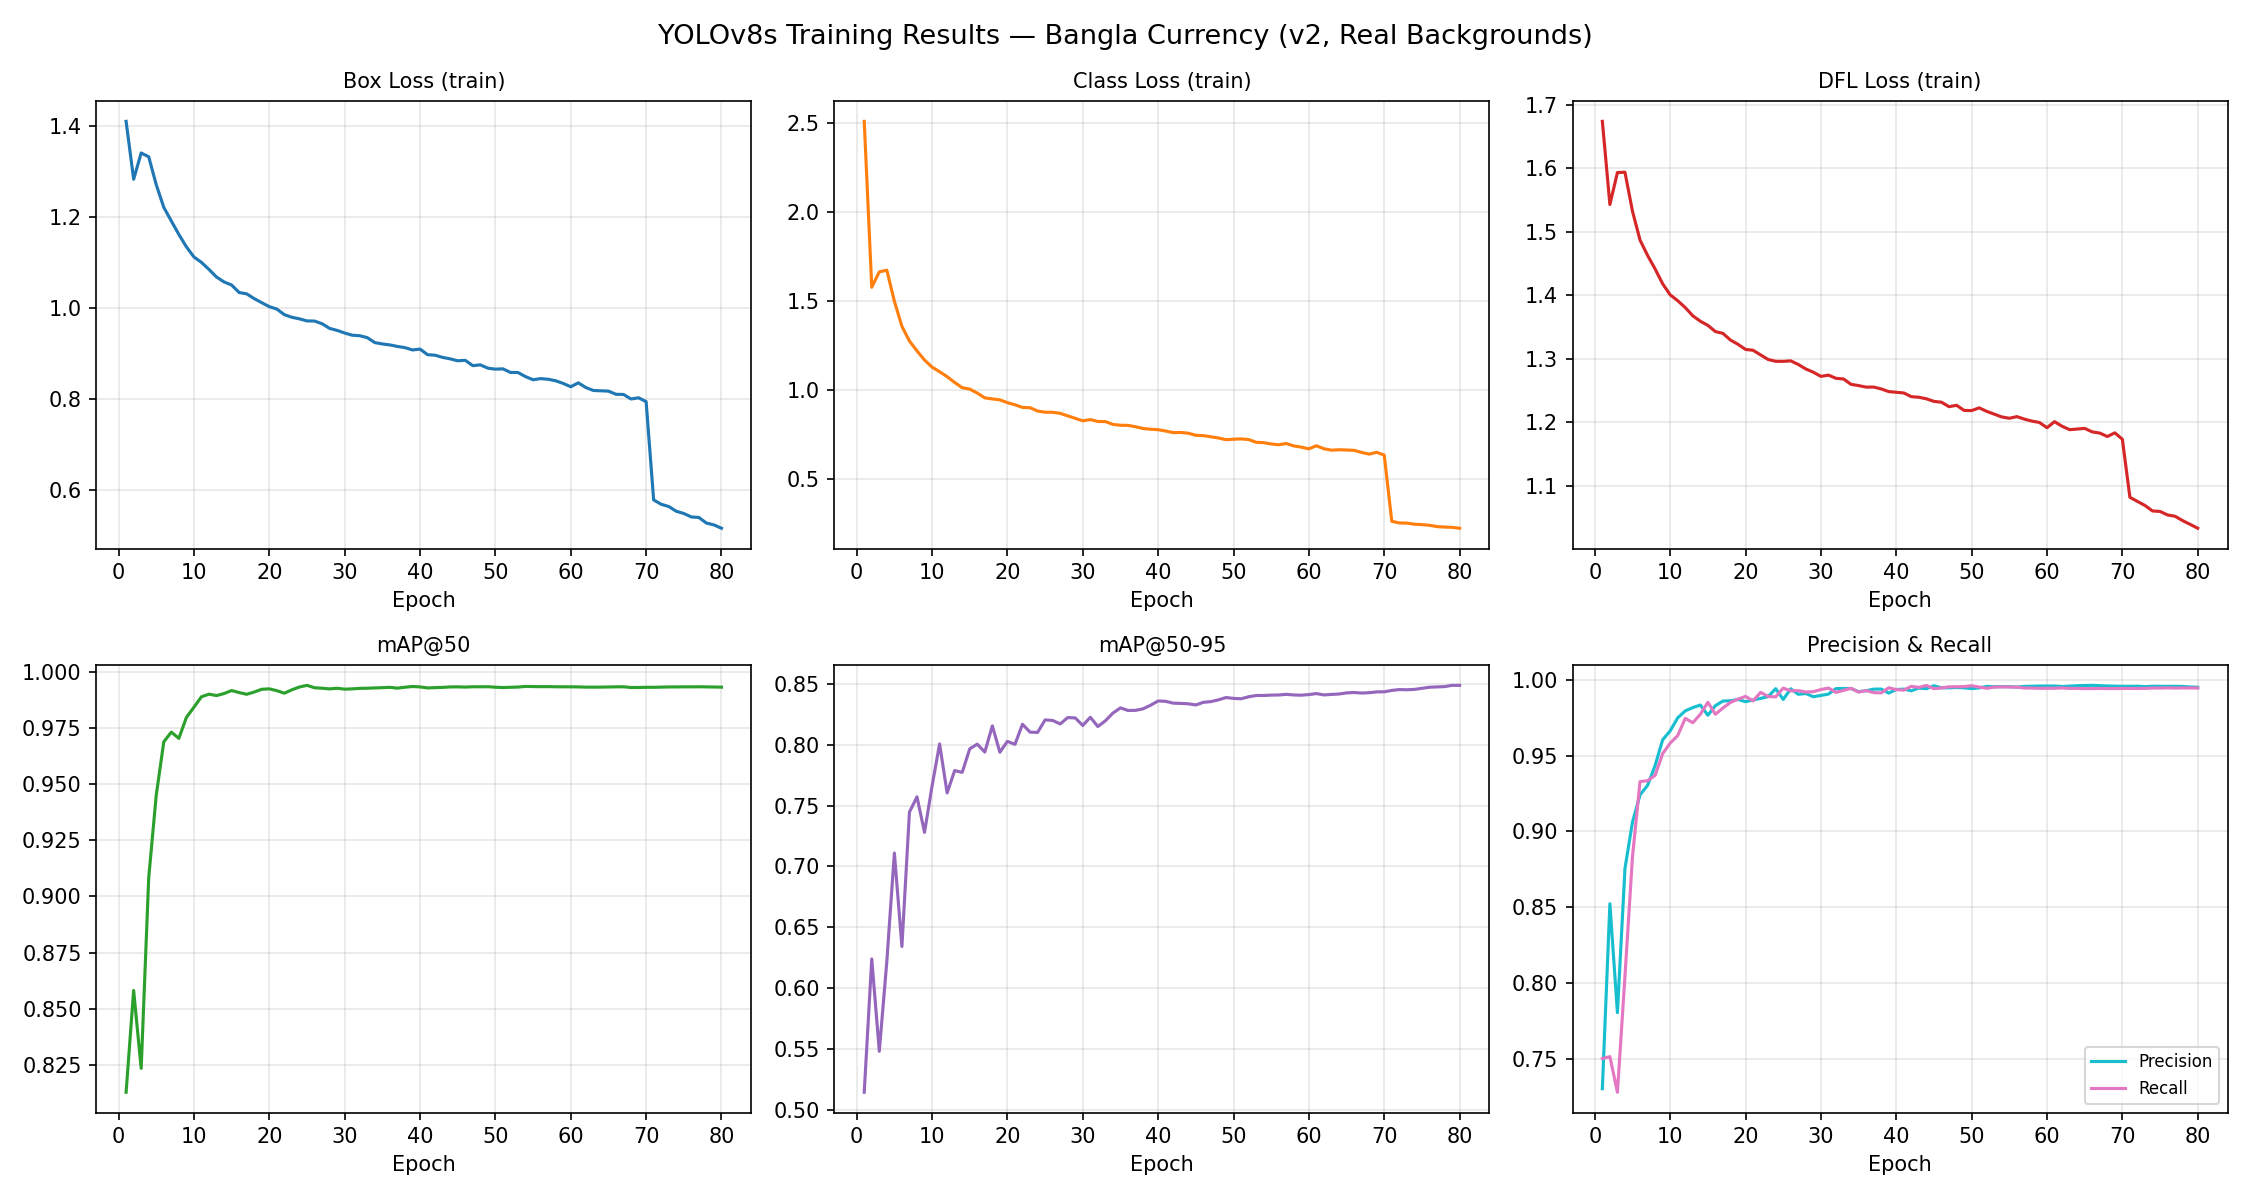
\includegraphics[width=\textwidth]{fig_training_curves.png}
    \caption{Training curves of the YOLOv8s Taka detector: box, class and DFL losses (top) and mAP@0.5, mAP@0.5:0.95, precision and recall (bottom) against epoch}
    \label{fig:traincurves}
\end{figure}

\subsection{Results on Held-Out Composites}
Table~\ref{tab:det_overall} reports the final performance on the 2,238 held-out test composites.

\begin{table}[!htbp]
\centering
\caption{Taka detection performance on the synthetic test set (2,238 images)}
\label{tab:det_overall}
\begin{tabular}{|l|c|}
\hline
\textbf{Metric} & \textbf{Value} \\ \hline
Precision & 0.998 \\ \hline
Recall & 0.997 \\ \hline
mAP@0.5 & 0.995 \\ \hline
mAP@0.5:0.95 & 0.847 \\ \hline
Inference time (RTX 4060 laptop GPU) & 7.3 ms / image ($\approx$135 FPS) \\ \hline
Pre-process / post-process time & 1.7 ms / 1.7 ms \\ \hline
\end{tabular}
\end{table}

A later re-validation of the same weights on the locally available validation data gave mAP@0.5 = 0.994, mAP@0.5:0.95 = 0.844, precision 0.991 and recall 0.992, which agrees with the original numbers. The gap between mAP@0.5 (0.995) and mAP@0.5:0.95 (0.847) shows that the detector almost always finds and correctly names the note, but that the box edges are less precise at strict IoU thresholds. One plausible reason is the slight anti-aliasing at the pasted, warped note borders, which does not correspond to a sharp physical edge.

\begin{table}[!htbp]
\centering
\caption{Per-denomination detection metrics on the synthetic test set}
\label{tab:det_perclass}
\begin{tabular}{|l|c|c|c|c|c|}
\hline
\textbf{Class} & \textbf{Instances} & \textbf{Precision} & \textbf{Recall} & \textbf{mAP@0.5} & \textbf{mAP@0.5:0.95} \\ \hline
2 Taka & 180 & 0.998 & 1.000 & 0.995 & 0.838 \\ \hline
5 Taka & 264 & 0.998 & 0.996 & 0.995 & 0.844 \\ \hline
10 Taka & 172 & 0.995 & 0.988 & 0.995 & 0.848 \\ \hline
20 Taka & 192 & 0.998 & 1.000 & 0.995 & 0.847 \\ \hline
50 Taka & 172 & 1.000 & 0.993 & 0.995 & 0.851 \\ \hline
100 Taka & 228 & 0.999 & 1.000 & 0.995 & 0.845 \\ \hline
200 Taka & 172 & 0.999 & 1.000 & 0.995 & 0.843 \\ \hline
500 Taka & 500 & 1.000 & 1.000 & 0.995 & 0.853 \\ \hline
1000 Taka & 172 & 0.994 & 1.000 & 0.995 & 0.858 \\ \hline
\textbf{All} & \textbf{2,052} & \textbf{0.998} & \textbf{0.997} & \textbf{0.995} & \textbf{0.847} \\ \hline
\end{tabular}
\end{table}

Results are uniformly strong across the nine classes (Table~\ref{tab:det_perclass}), including the smallest source class (10 Taka, 419 source images), so the model does not simply favour the most frequent class (500 Taka, 1,243 source images). Because mAP@0.5 rounds to 0.995 for every class, mAP@0.5:0.95 (0.838--0.858) is the more informative column for comparing denominations. The normalised confusion matrix (Figure~\ref{fig:det_confusion}) is almost perfectly diagonal; the remaining errors are missed or spurious detections against the background, not confusions between two denominations. For a currency reader this is the safer failure mode: the glass may ask the user to hold the note again, but it rarely names the wrong value.

\begin{figure}[H]
    \centering
    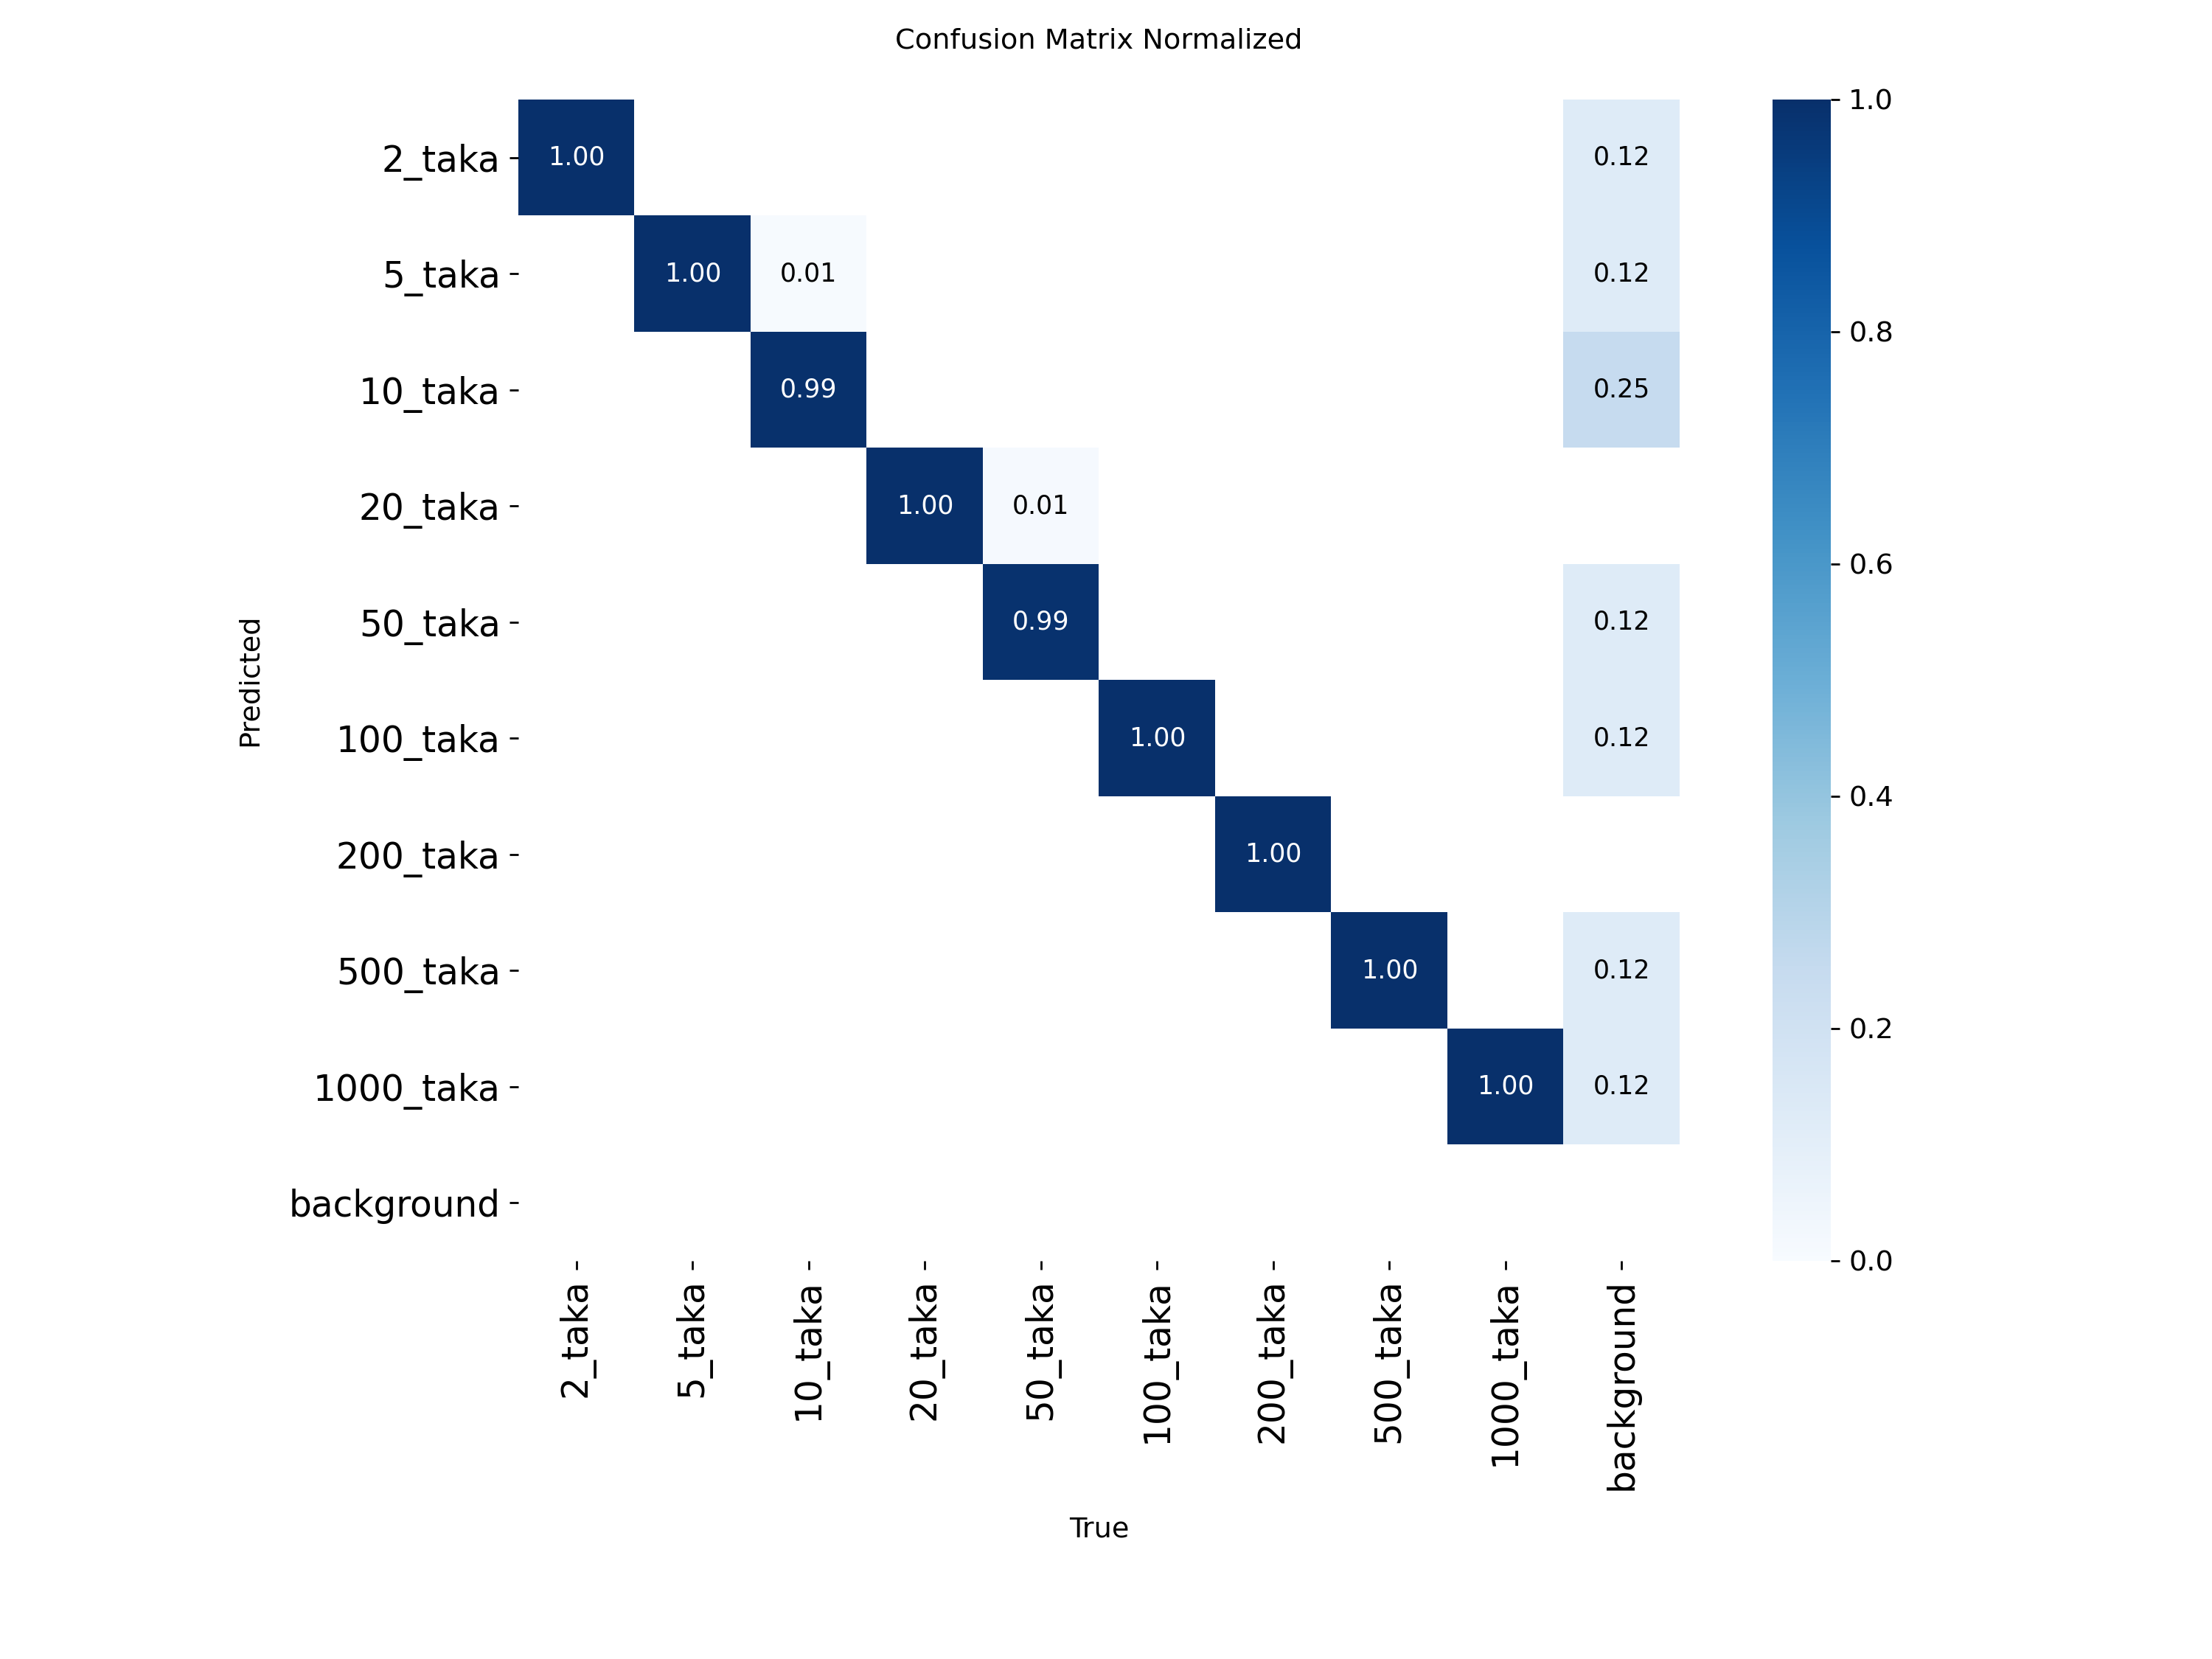
\includegraphics[width=0.7\textwidth]{fig_confusion_matrix.png}
    \caption{Normalised confusion matrix of the Taka detector on the synthetic test set}
    \label{fig:det_confusion}
\end{figure}

\begin{figure}[H]
    \centering
    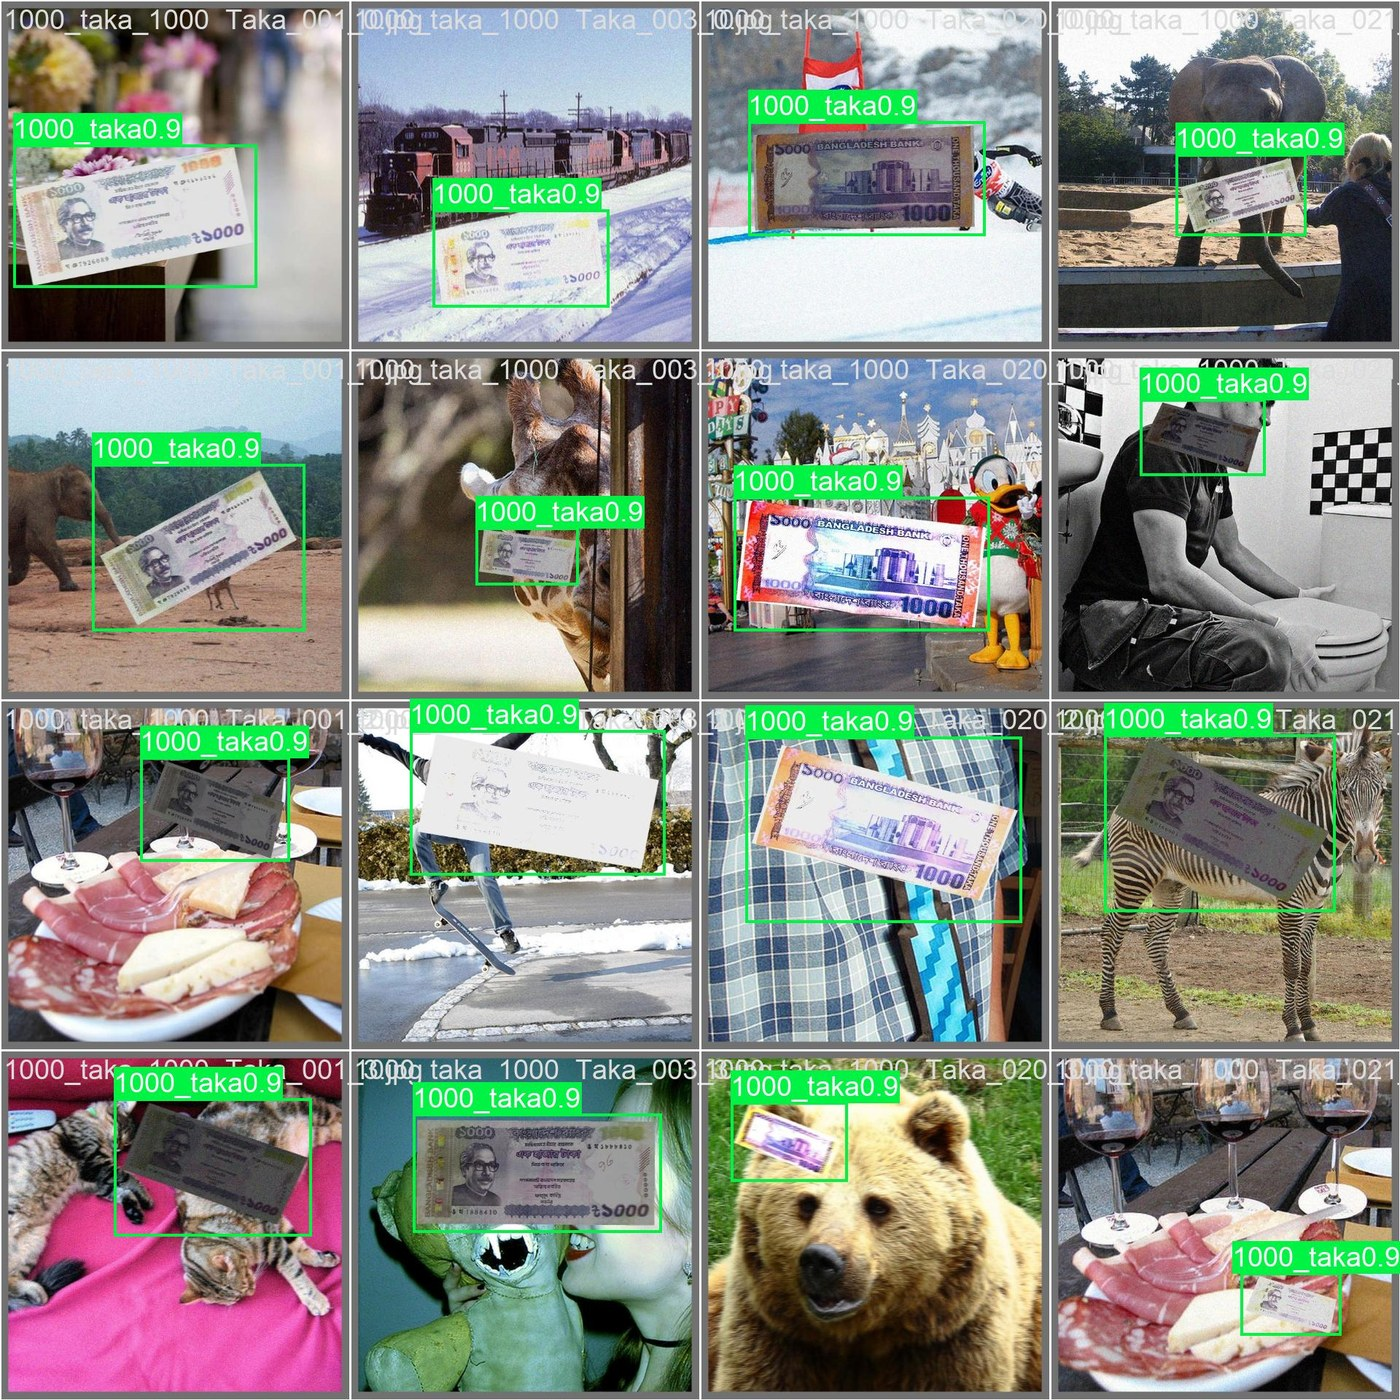
\includegraphics[width=0.95\textwidth]{fig_qualitative.jpg}
    \caption{Example predictions on held-out composites with predicted class and confidence. The note is localised across different scales, rotations and backgrounds.}
    \label{fig:qualitative}
\end{figure}

\subsection{Results on Raw Phone Photographs (Source Domain, Not Held Out)}
Table~\ref{tab:wild} shows the result of the same detector on the 450 raw phone photographs (50 per denomination). A note counts as \textit{detected} if any box is predicted, and as \textit{correct} if the top-scoring box has the true denomination.

\begin{table}[!htbp]
\centering
\caption{Taka detection on 450 raw phone photographs (50 per denomination). Source-domain check: these photographs come from the detector's training source and are not held out. Independent results: Table~\ref{tab:external}.}
\label{tab:wild}
\begin{tabular}{|l|c|c|c|p{4.6cm}|}
\hline
\textbf{True class} & \textbf{Detected} & \textbf{Correct} & \textbf{Top-1 (\%)} & \textbf{Errors} \\ \hline
2 Taka & 49 & 47 & 94.0 & 2 read as 5 Taka, 1 missed \\ \hline
5 Taka & 50 & 50 & 100.0 & -- \\ \hline
10 Taka & 48 & 48 & 96.0 & 2 missed \\ \hline
20 Taka & 50 & 50 & 100.0 & -- \\ \hline
50 Taka & 48 & 46 & 92.0 & 1 as 5 Taka, 1 as 500 Taka, 2 missed \\ \hline
100 Taka & 48 & 48 & 96.0 & 2 missed \\ \hline
200 Taka & 50 & 50 & 100.0 & -- \\ \hline
500 Taka & 50 & 50 & 100.0 & -- \\ \hline
1000 Taka & 50 & 47 & 94.0 & 3 read as 500 Taka \\ \hline
\textbf{Overall} & \textbf{443 (98.4\%)} & \textbf{436} & \textbf{96.9} & \textbf{7 missed, 7 wrong value} \\ \hline
\end{tabular}
\end{table}

On raw photographs the detector finds 98.4\% of the notes and names 96.9\% correctly. Because these photographs come from the same source as the training foregrounds, this number does not measure transfer to new notes; the independent collections in Table~
ef{tab:external} do (91.5\% on Bangla Money). The errors are informative: 2 and 5 Taka are both small, similar-coloured notes, and the 1000 and 500 Taka notes share a similar layout and portrait. As explained in Chapter~\ref{chap:dataset}, some physical notes in this set may also occur in the training foregrounds, so this is an optimistic estimate. The 450 images were drawn from the raw folder without excluding the photographs used as training foregrounds, so this table is a source-domain check, not a test; the independent results below replace it as the real-photograph result.

\subsection{Results on Independent Photographs}
Two public collections that were never used for training or selection were scored with the same detector at confidence 0.25 (Table~\ref{tab:external}). A third, ``A Diverse Image Dataset for Bangladeshi Currency Recognition'', was excluded because its files are byte-identical to the training source.

\begin{table}[!htbp]
\centering
\caption{Taka detection on independent photograph collections}
\label{tab:external}
\begin{tabular}{|l|c|p{7cm}|}
\hline
\textbf{Set} & \textbf{n} & \textbf{Result} \\ \hline
Bangla Money (Kaggle), 8 denominations & 1,536 & 91.5\% correct denomination; no note found 3.9\%; 95.2\% correct when a note is found \\ \hline
NSTU-BDTAKA detection test & 186 & class-agnostic AP@0.5 0.796; precision 0.832, recall 0.694 \\ \hline
NSTU-BDTAKA hand-held close-ups & 1,144 & 18.5\% correct denomination; no note found 66.9\% \\ \hline
Bangla Money 1-Taka notes (unknown class) & 101 & 57 not detected; 44 announced as a known note (37 as 5 Taka) \\ \hline
\end{tabular}
\end{table}

The detector transfers to full-note photographs taken by other people, with 1000 Taka the weakest class (78.4\%, mostly read as 500 Taka). It does not transfer to close-ups in which fingers cover part of a folded note, and it has no ``unknown note'' output.

\subsection{Fall-Back Classifier}
The MobileNetV3-Small classifier used as a fall-back reached a best validation accuracy of 99.2\% on the nine-class BanglaTaka crops. This is a whole-note classification score on clean crops, not a detection score in a scene.

\subsection{Comparison with Related Work}
Compared with published detectors (Table~\ref{tab:currency_compare}), our mAP@0.5:0.95 of 0.847 on composites is higher than the 0.804 reported for a custom-head YOLOv8n multi-currency model \cite{yolov8nse}, and our precision and recall (0.998/0.997) are higher than the 0.95/0.93 of the YOLOv5 baseline trained on 3,111 manually annotated images \cite{nstubdtaka2024}. Our labelled dataset is about seven times larger and required no manual annotation. However, the test sets are different and our headline scores are on synthetic images, so the comparison indicates competitiveness, not superiority on a common benchmark.

\section{Taka Authentication Performance}

\subsection{Accuracy for One to Six Views}
All authentication models were evaluated on the same 208 test notes with the first $k$ views, for $k = 1,\dots,6$. Table~\ref{tab:auth_views} compares the CNN+ViT baseline, which was trained with all six views, with the prefix-robust model (PRMVT).

\begin{table}[!htbp]
\centering
\caption{Authentication accuracy on 208 test notes with the first $k$ views (seed 42)}
\label{tab:auth_views}
\begin{tabular}{|c|c|c|c|}
\hline
\textbf{Views} & \textbf{CNN+ViT baseline} & \textbf{PRMVT (proposed)} & \textbf{Gain (points)} \\ \hline
1 & 73.56\% & \textbf{97.12\%} & +23.6 \\ \hline
2 & 87.02\% & \textbf{98.08\%} & +11.1 \\ \hline
3 & 91.35\% & \textbf{98.08\%} & +6.7 \\ \hline
4 & 91.83\% & \textbf{98.08\%} & +6.3 \\ \hline
5 & 89.90\% & \textbf{98.56\%} & +8.7 \\ \hline
6 & 91.83\% & \textbf{98.08\%} & +6.3 \\ \hline
\end{tabular}
\end{table}

The baseline is much weaker with one view (73.6\%) than with six (91.8\%). An earlier version of our fusion model trained only on six views showed the same problem even more strongly: 96.6\% with six views but only 68.8\% with one view. This is the view-count distribution shift described in Section~\ref{sec:method}. The prefix-robust protocol removes it: PRMVT stays between 97.1\% and 98.6\% for every number of views. The difference to the baseline is statistically significant under McNemar's test at one view ($p = 4.3\times10^{-11}$) and at six views ($p = 0.0020$). After a Bonferroni correction over 36 algorithm-by-view comparisons, the one-, two-, three- and five-view gains remain significant, while the four- and six-view gains do not; this correction is reported so that the six-view improvement is not overstated. The PRMVT numbers in this chapter were re-evaluated after a numerical fault was fixed: the entropy of a fully confident prediction was computed as $0 \cdot \log 0$, which is undefined, and the model then reported a probability of 0.5 for that note. The fault affected 23 of the 208 test notes at six views and made the earlier figures slightly lower (six-view accuracy 97.6\% instead of 98.1\%).

\begin{figure}[H]
    \centering
    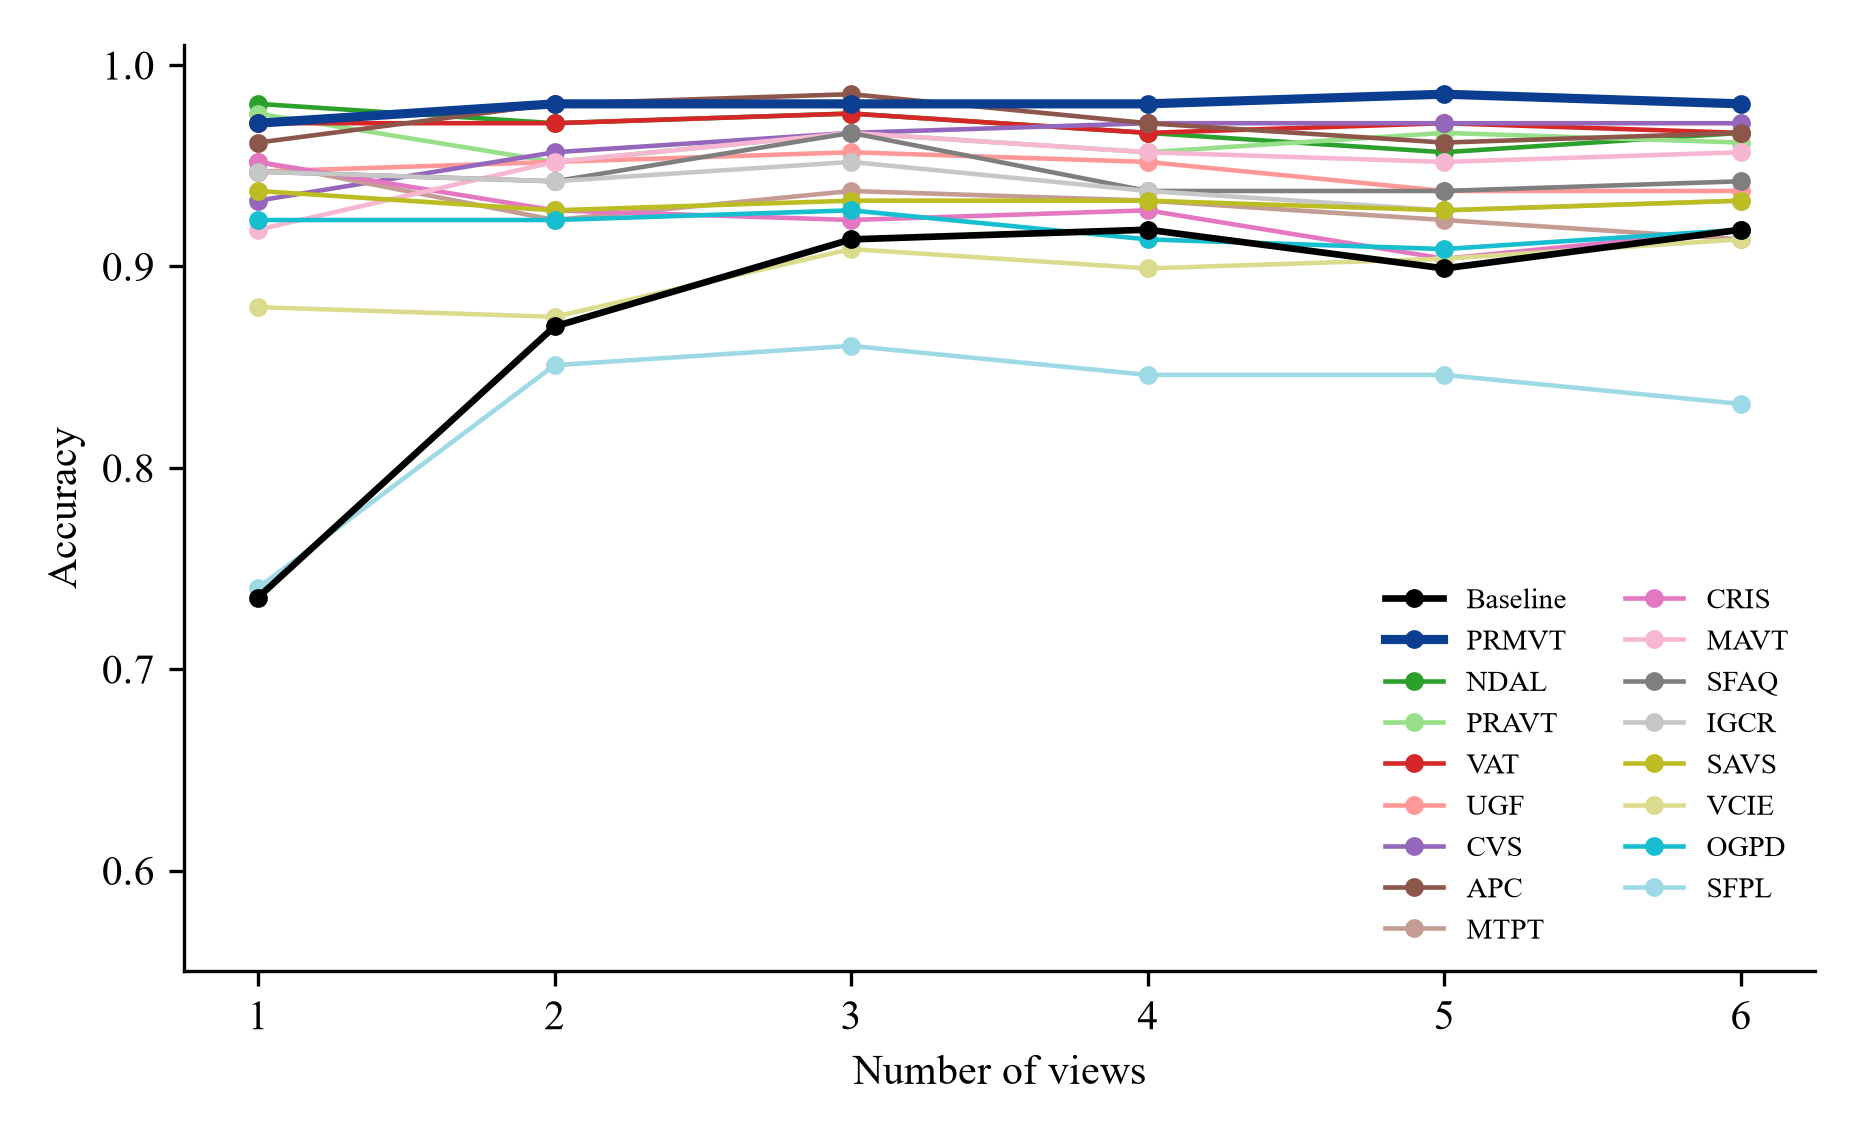
\includegraphics[width=0.85\textwidth]{fig_auth_views.png}
    \caption{Authentication accuracy against the number of views for the CNN+ViT baseline, PRMVT and the other training variants tried in this project}
    \label{fig:auth_views}
\end{figure}

\subsection{Repeatability over Seeds}
PRMVT was trained with three random seeds (42, 43, 44). The mean accuracy was 96.5\% (standard deviation 1.6 points) with one view and 98.1\% (standard deviation 1.0 point) with six views; the lowest mean over the six view counts was 96.5\% (Table~\ref{tab:multiseed}). The result is therefore not a lucky seed, although three seeds is a small sample.

\begin{table}[!htbp]
\centering
\caption{PRMVT accuracy over three seeds (mean $\pm$ standard deviation)}
\label{tab:multiseed}
\begin{tabular}{|c|c|c|c|c|c|c|}
\hline
\textbf{Views} & 1 & 2 & 3 & 4 & 5 & 6 \\ \hline
\textbf{Mean (\%)} & 96.47 & 98.40 & 98.08 & 97.60 & 98.56 & 98.08 \\ \hline
\textbf{SD (points)} & 1.55 & 0.56 & 0.48 & 0.83 & 0.48 & 0.96 \\ \hline
\end{tabular}
\end{table}

\subsection{Other Metrics and Calibration}
For the six-view operating point of the fixed-count fusion model, the improvement over the baseline is consistent across metrics: accuracy 0.966 vs.\ 0.918, macro-F1 0.966 vs.\ 0.914, balanced accuracy 0.965 vs.\ 0.906, ROC-AUC 0.989 vs.\ 0.971, and expected calibration error (ECE) 0.030 vs.\ 0.079. A lower ECE means that the confidence reported by the model matches its real accuracy better, which is important if the glass tells the user ``probably counterfeit''. For PRMVT, the six-view ECE without any calibration is 0.015, so its confidence is already well matched to its accuracy; calibration maps fitted on the validation set (temperature scaling and a quality-aware map) do not improve on it (0.017--0.018). An earlier uncalibrated value of 0.061 was caused by the numerical fault described above, which reported a probability of 0.5 for notes the model was certain about. The confusion matrices (Figure~\ref{fig:auth_confusion}) show that PRMVT mainly removes the baseline's errors on counterfeit notes that were accepted as genuine (a fraction of 0.07 of all test notes for the baseline, 0.01 for PRMVT).

\begin{figure}[H]
    \centering
    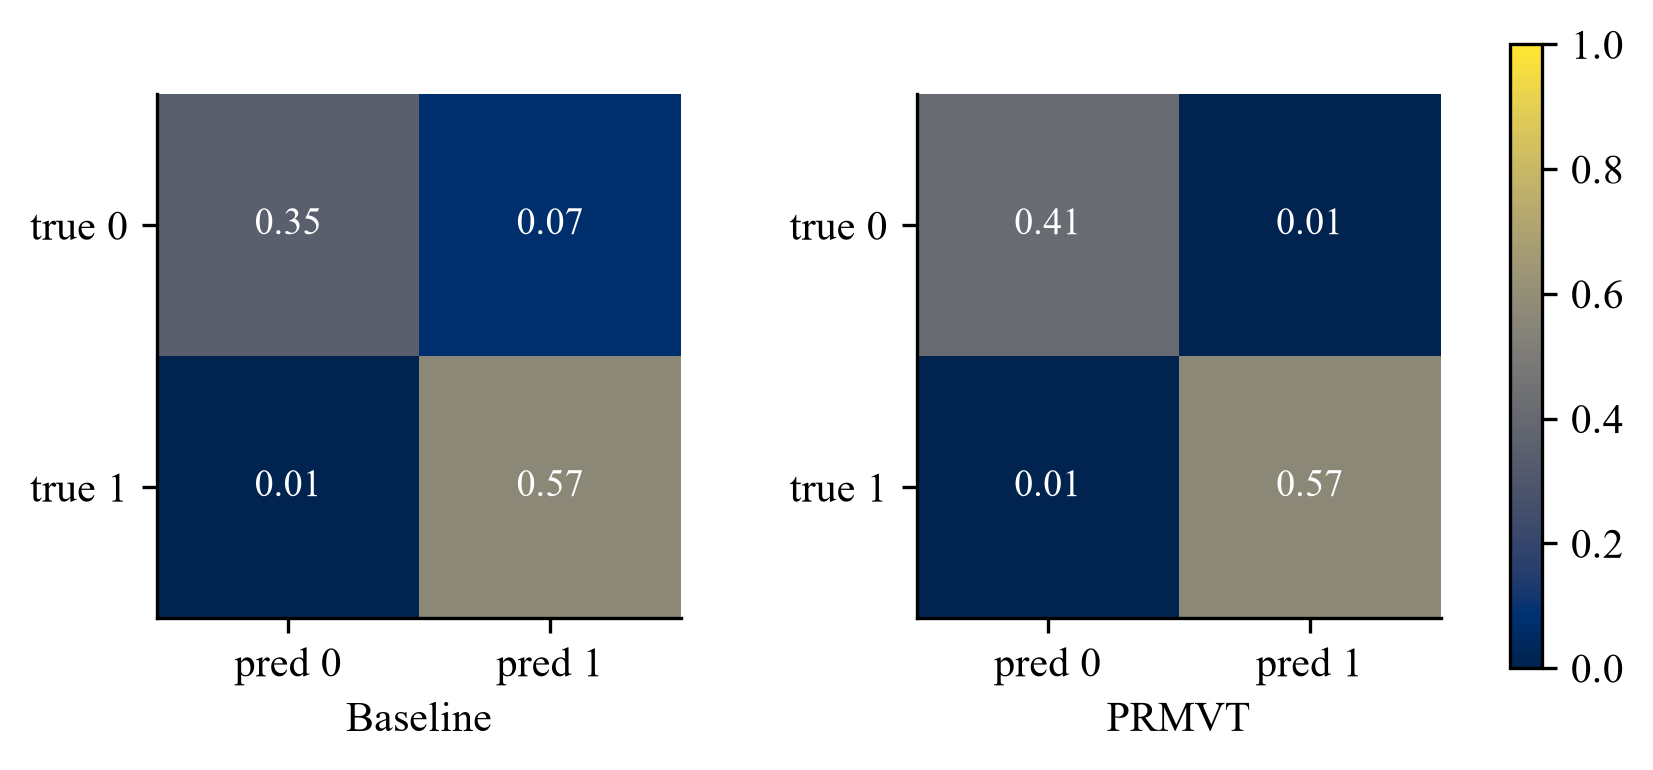
\includegraphics[width=0.75\textwidth]{fig_auth_confusion.png}
    \caption{Normalised confusion matrices of the baseline and PRMVT at six views (0 = counterfeit, 1 = genuine)}
    \label{fig:auth_confusion}
\end{figure}

\subsection{Robustness to Image Corruptions}
The models were tested under 13 image corruptions at several strengths (Figure~\ref{fig:auth_robust}). PRMVT is almost unaffected by Gaussian and motion blur, JPEG compression, scale change and sensor noise. It is clearly sensitive to low light, strong brightness, rotation, perspective and especially occlusion: at an occlusion of 55\% of the image, six-view accuracy fell to 51.9\%, which is worse than the baseline (81.3\%). Fine-tuning with low-light augmentation raised accuracy at the darkest setting (brightness factor 0.2) to 93.75\% while keeping 98.6\% on clean images, but a first, short occlusion fine-tune did not fix occlusion (68.3\%, with clean accuracy falling to 90.9\%). An analysis on the validation set showed why: under occlusion PRMVT called most genuine notes counterfeit, because a covered region looks like a missing security feature, and the earlier fine-tunes had kept the CNN frozen and trained only briefly. A longer fine-tune in which every view is randomly covered and the last CNN blocks can adapt, with the epoch chosen on the validation set, raised accuracy at 55\% occlusion to 88.5\% (87.0\% $\pm$ 2.2 over three seeds, 88.9\% for their average) while clean accuracy stayed at 98--99\%. This is still below 90\%. If the model is allowed to answer only when it is at least 99\% confident and otherwise asks the user to reposition the note, it answers about half of the occluded notes with 99.0\% accuracy, and wrong verdicts fall from 11.1\% to 0.5\% of occluded notes. These tests use a black rectangle; a real finger is neither black nor rectangular, so occlusion by fingers remains the main open failure mode.

\begin{figure}[H]
    \centering
    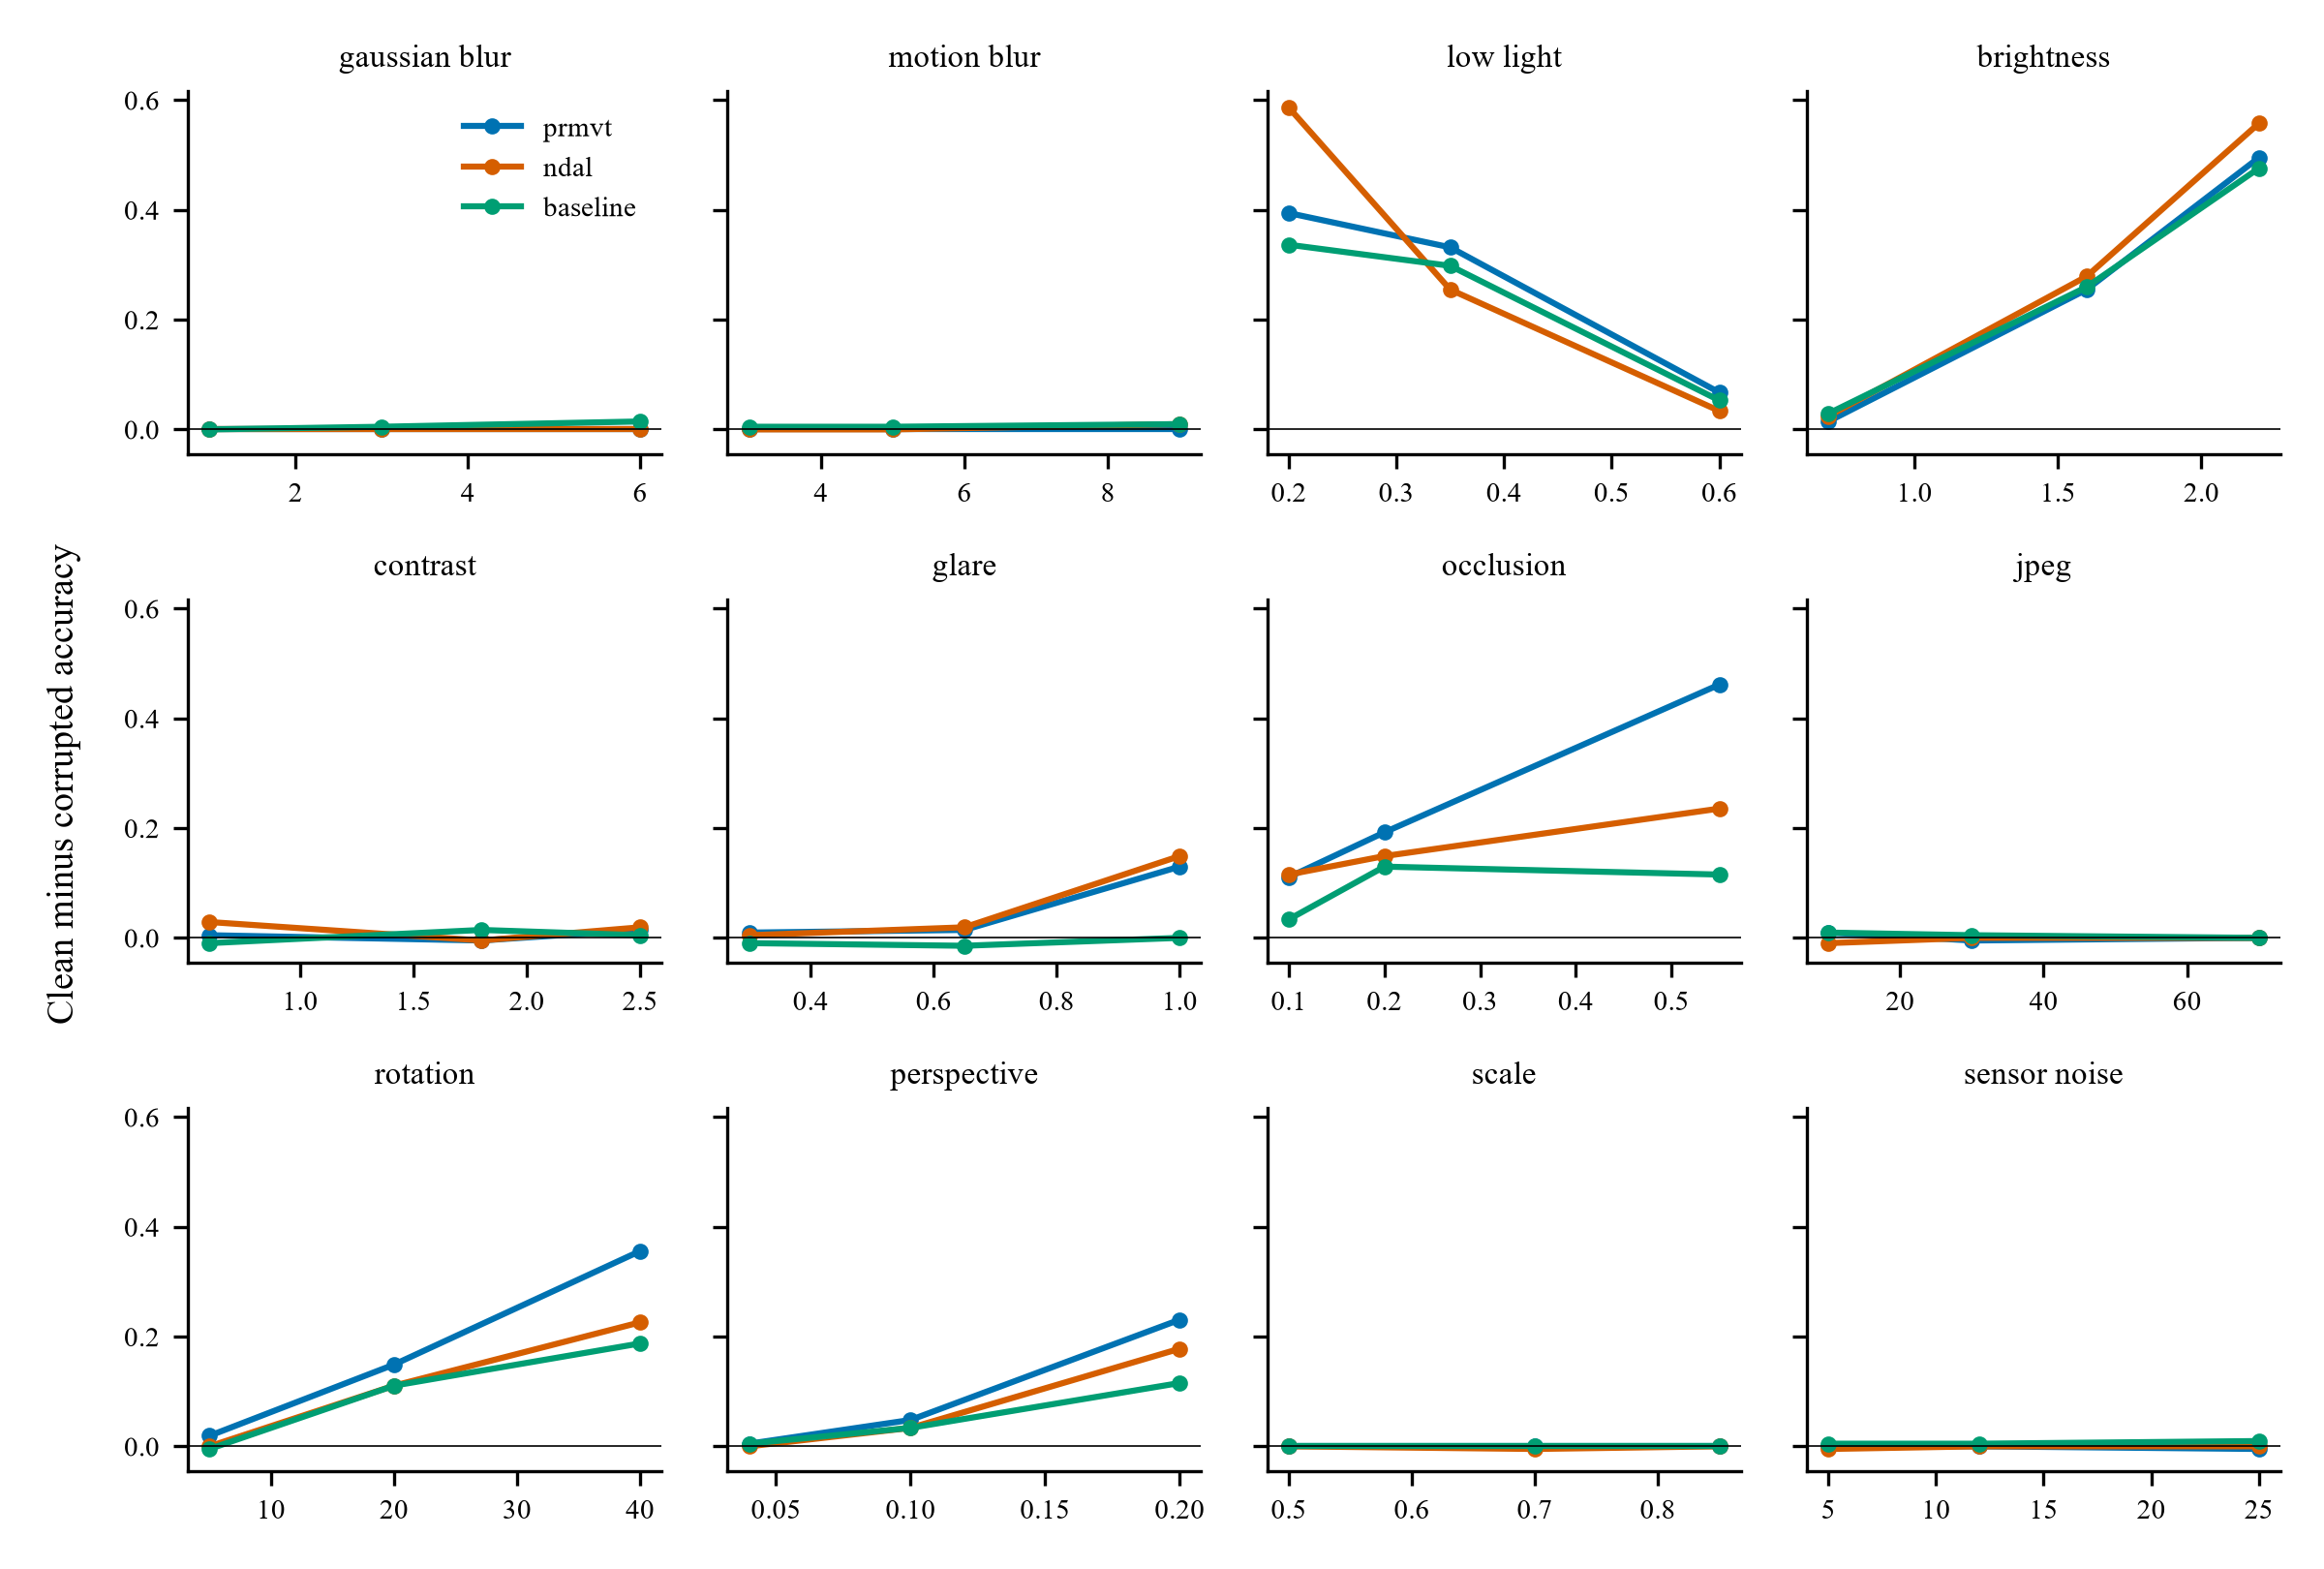
\includegraphics[width=\textwidth]{fig_auth_robustness.png}
    \caption{Accuracy drop (clean minus corrupted accuracy) at six views under 12 corruptions for PRMVT, the NDAL variant and the baseline}
    \label{fig:auth_robust}
\end{figure}

\subsection{Authentication on Whole-Note Photographs}
\label{sec:jaal_deployed}
The glass applies the authenticator to one crop of the note found by the detector, not to the close-up views it was trained on. This deployed path was scored on photographs that were not used for training or selection (Table~\ref{tab:jaal_deployed}).

\begin{table}[!htbp]
\centering
\caption{Deployed genuine/counterfeit verdict on whole-note photographs (one crop, threshold 0.5)}
\label{tab:jaal_deployed}
\begin{tabular}{|l|c|c|}
\hline
\textbf{Set} & \textbf{Notes judged} & \textbf{Wrong verdict (95\% Wilson CI)} \\ \hline
Bangla Money, genuine & 1,464 & 47.7\% (45.2--50.3) \\ \hline
BanglaTaka raw, genuine & 441 & 59.2\% (54.5--63.7) \\ \hline
Counterfeit-currency set, genuine & 1,187 & 20.4\% (18.2--22.8) \\ \hline
Counterfeit-currency set, counterfeit & 75 & 40.0\% (29.7--51.3) \\ \hline
\end{tabular}
\end{table}

A genuine note called counterfeit, or a counterfeit called genuine, is the most harmful error for a blind user. The glass therefore no longer speaks the verdict: it announces the denomination followed by ``the counterfeit check was not done''. The high close-up accuracy in Table~\ref{tab:auth_views} does not carry over to whole-note crops.

\subsection{Other Training Variants and Negative Results}
Fifteen other training variants were tried on the same split (Figure~\ref{fig:auth_views}). Several of them reach 95--98\% at one view, for example a focal-style loss variant (NDAL) \cite{focalloss} with 98.1\% at one view, so the accuracy alone does not single out one algorithm; the common factor is that all of them see varying numbers of views during training. Some variants failed: a simulated federated version stayed at 74.0\% with one view and below the baseline from two views on, and one retrained variant became worse than its first version. We also tried learned policies that choose which view to capture next and when to stop (rules based on image quality, confidence, diversity and uncertainty, and a cost-aware rule). On PRMVT, averaged over three seeds, none of them beat simply taking the views in their fixed order (96.5\% with one view and 97.6--98.6\% with two to six): the learned rules picked a weaker first view and reached 89.3--90.2\% with one view, and the cost-aware rule with early stopping stopped after one view at 89.3\%. A prefix stopping rule on the fixed order reached 97.1\% with an average of 1.01 views, which is simply because PRMVT is already accurate with one view. Earlier, much lower figures for these policies (down to 42\%) were caused by evaluation faults that have since been fixed, not by the policies themselves. These negative results are reported so that the method is not presented as better than it is.

\subsection{Speed}
On the RTX~3050 laptop GPU, one six-view authentication takes a median of 42.6~ms (95th percentile 69.5~ms). The model file is 14.5~MB. The time on the Raspberry Pi~5 has not been measured.

\section{Emotion Recognition Performance}

Several models were trained and compared on the official RAF-DB test set (Table~\ref{tab:emotion_runs}). The EfficientNet-V2-S model with flip test-time augmentation gave the best accuracy, 86.5\%, and is used in the system.

\begin{table}[!htbp]
\centering
\caption{Emotion recognition models compared during development}
\label{tab:emotion_runs}
\begin{tabular}{|p{4.8cm}|p{4.0cm}|c|c|}
\hline
\textbf{Model} & \textbf{Test set} & \textbf{Accuracy} & \textbf{Used} \\ \hline
FER+ ONNX & FER-2013 hold-out, n = 5,741 & 57.9\% & Fall-back \\ \hline
MobileNetV3-Large & RAF-DB official test, n = 3,068 & 81.0\% & Replaced \\ \hline
ViT (face-expression) fine-tune & RAF-DB official test & 84.3\% (peak) & No \\ \hline
EfficientNet-B2 (AffectNet) fine-tune & RAF-DB official test & 85.2\% (then over-fit) & No \\ \hline
\textbf{EfficientNet-V2-S + flip TTA} & \textbf{RAF-DB official test} & \textbf{86.5\%} & \textbf{Yes} \\ \hline
\end{tabular}
\end{table}

\begin{table}[!htbp]
\centering
\caption{Per-class results of the EfficientNet-V2-S emotion model on RAF-DB (n = 3,068)}
\label{tab:emotion_perclass}
\begin{tabular}{|l|c|c|c|c|}
\hline
\textbf{Class} & \textbf{Support} & \textbf{Precision} & \textbf{Recall} & \textbf{F1} \\ \hline
Happy & 1,185 & 0.946 & 0.925 & 0.936 \\ \hline
Sad & 478 & 0.839 & 0.839 & 0.839 \\ \hline
Angry & 162 & 0.789 & 0.809 & 0.799 \\ \hline
Surprise & 329 & 0.867 & 0.872 & 0.870 \\ \hline
Fear & 74 & 0.774 & 0.554 & 0.646 \\ \hline
Disgust & 160 & 0.671 & 0.588 & 0.627 \\ \hline
Neutral & 680 & 0.815 & 0.890 & 0.851 \\ \hline
\textbf{Macro average} & \textbf{3,068} & \textbf{0.815} & \textbf{0.782} & \textbf{0.795} \\ \hline
\end{tabular}
\end{table}

The accuracy is 86.5\% and the macro-F1 is 0.795 (Table~\ref{tab:emotion_perclass}). Happy, surprise, neutral and sad are recognised well; fear and disgust are the weakest classes because they have the fewest training images and are often confused with sad and neutral (Table~\ref{tab:emotion_cm}). The published state of the art on this split is about 92\% (POSTER~V2 \cite{posterv2}), so our model is a reasonable but not state-of-the-art recogniser. For adaptive speech, the most important decision is whether a person looks stressed (sad, fear, anger, disgust) or not, which is less demanding than the full seven-class task.

\begin{table}[!htbp]
\centering
\caption{Confusion matrix of the EfficientNet-V2-S emotion model on the RAF-DB official test set (rows: true class, columns: predicted class)}
\label{tab:emotion_cm}
\begin{tabular}{|l|c|c|c|c|c|c|c|}
\hline
\textbf{True / Pred.} & \textbf{Hap.} & \textbf{Sad} & \textbf{Ang.} & \textbf{Sur.} & \textbf{Fear} & \textbf{Dis.} & \textbf{Neu.} \\ \hline
\textbf{Happy} & \textbf{1096} & 11 & 8 & 12 & 1 & 11 & 46 \\ \hline
\textbf{Sad} & 14 & \textbf{401} & 5 & 4 & 1 & 14 & 39 \\ \hline
\textbf{Angry} & 7 & 2 & \textbf{131} & 4 & 4 & 4 & 10 \\ \hline
\textbf{Surprise} & 6 & 8 & 3 & \textbf{287} & 5 & 5 & 15 \\ \hline
\textbf{Fear} & 3 & 8 & 5 & 11 & \textbf{41} & 2 & 4 \\ \hline
\textbf{Disgust} & 11 & 15 & 13 & 4 & 0 & \textbf{94} & 23 \\ \hline
\textbf{Neutral} & 21 & 33 & 1 & 9 & 1 & 10 & \textbf{605} \\ \hline
\end{tabular}
\end{table}

\section{Text Recognition Performance}

\subsection{OCR Error Rates}
OCR quality is measured by the character error rate (CER) and word error rate (WER), the edit distance between recognised text and ground truth divided by the length of the ground truth. Table~\ref{tab:ocr} shows the results of EasyOCR with our pre-processing on the 80-phrase test set.

\begin{table}[!htbp]
\centering
\caption{OCR error rates of EasyOCR (Bangla + English) with CLAHE pre-processing}
\label{tab:ocr}
\begin{tabular}{|l|c|c|c|}
\hline
\textbf{Language} & \textbf{Samples} & \textbf{CER} & \textbf{WER} \\ \hline
English & 40 & 3.2\% & 10.4\% \\ \hline
Bangla & 40 & 27.8\% & 57.9\% \\ \hline
\textbf{Overall} & \textbf{80} & \textbf{15.5\%} & \textbf{34.2\%} \\ \hline
\end{tabular}
\end{table}

English text is read almost perfectly (3.2\% CER), but Bangla text has a CER of 27.8\%: on average more than one character in four is wrong, and more than half of the words contain an error. Inspection of the outputs shows that most Bangla errors are in vowel signs (\textit{kar}) that are dropped or placed on the wrong consonant, and in conjunct consonants (\textit{juktakkhor}) that are split into separate letters. The consonant skeleton of a word is usually correct, so a listener can often still guess the word, but the result is not reliable enough for unfamiliar text. A lexicon-based correction was tried; because its word list included the test phrases, its near-zero error is not a valid measurement and is not reported as a result.

\subsection{Handwritten Bangla Character Recognition}
The CNN trained on Ekush reached 90.0\% test accuracy on 38,608 characters from 305 unseen writers (best validation accuracy 91.1\%). Accuracy was 94.3\% for digits, 94.2\% for modifiers, 93.1\% for vowels, 89.9\% for consonants and 87.7\% for conjuncts. The lower accuracy for conjuncts confirms that compound characters are the hardest part of Bangla recognition, which is also the main source of the OCR errors above.

\section{Object Detection Performance}
The COCO-pretrained YOLOv8s model reached mAP@0.5 = 0.604 on the 250-image COCO val2017 subset (77 classes present). Large, distinctive objects such as buses, laptops, suitcases, dogs and beds had AP@0.5 above 0.90, while small or rare objects were weaker. The object mode reduces the effect of false alarms by using a confidence threshold of 0.50 and by announcing at most three objects per scan. Precision of the spoken announcements in real indoor use has not yet been measured.

\section{Processing Speed}
Table~\ref{tab:speed} summarises the measured speed. On a laptop CPU (AMD Ryzen~7 5800H, all three formats measured in the same run), the Taka detector takes a median of 109~ms per 640$\times$640 image (9.2 FPS) with PyTorch weights, 139~ms with FP32 ONNX Runtime and 101~ms (9.9 FPS) with the INT8 ONNX model, which is also the smallest file. An earlier INT8 figure (199~ms, 11.5~MB) belonged to a defective export that detected no notes and has been replaced. None of these figures is a Raspberry Pi~5 measurement.

\begin{table}[!htbp]
\centering
\caption{Measured processing speed (Raspberry Pi~5 not measured)}
\label{tab:speed}
\begin{tabular}{|p{4.6cm}|p{4.2cm}|c|c|}
\hline
\textbf{Model} & \textbf{Hardware} & \textbf{Time} & \textbf{Size} \\ \hline
YOLOv8s Taka (PyTorch) & RTX 4060 laptop GPU & 7.3 ms & 22.5 MB \\ \hline
YOLOv8s Taka (PyTorch) & Laptop CPU (Ryzen 7 5800H) & 109 ms & 22.5 MB \\ \hline
YOLOv8s Taka (FP32 ONNX) & Laptop CPU (Ryzen 7 5800H) & 139 ms & 44.8 MB \\ \hline
YOLOv8s Taka (INT8 ONNX) & Laptop CPU (Ryzen 7 5800H) & 101 ms & 18.0 MB \\ \hline
PRMVT authenticator, 6 views & RTX 3050 laptop GPU & 42.6 ms (median) & 14.5 MB \\ \hline
All models & Raspberry Pi~5 & Not measured & -- \\ \hline
\end{tabular}
\end{table}

\section*{Calculation Methods and Full Working}

This section presents the formulas used in this chapter and a worked example for each main table.

\subsection*{1) Detection Precision, Recall and mAP (Table~\ref{tab:det_overall})}
With $TP$, $FP$ and $FN$ the numbers of true positives, false positives and false negatives at a given IoU threshold,
\[
\text{Precision} = \frac{TP}{TP+FP}, \qquad \text{Recall} = \frac{TP}{TP+FN}, \qquad
\text{IoU}(A,B) = \frac{|A\cap B|}{|A\cup B|}.
\]
The average precision (AP) of one class is the area under its precision--recall curve; mAP@0.5 is the mean AP over the 9 classes at IoU $\geq 0.5$, and mAP@0.5:0.95 is the mean over the ten IoU thresholds $0.50, 0.55, \dots, 0.95$.

\subsection*{2) Raw-Photograph Detection Rate and Top-1 Accuracy (Table~\ref{tab:wild})}
\[
\text{Detection rate} = \frac{\text{notes with at least one box}}{\text{all notes}} = \frac{450-7}{450} = \frac{443}{450} = 98.4\%,
\]
\[
\text{Top-1 accuracy} = \frac{\text{notes with correct top box}}{\text{all notes}} = \frac{436}{450} = 96.9\%,
\]
where $436 = 48+48+47+47+50+50+50+46+50$ is the sum of the correct notes over the nine denominations.

\subsection*{3) Authentication Accuracy and McNemar's Test (Table~\ref{tab:auth_views})}
With 208 test notes, one-view PRMVT accuracy $= 202/208 = 97.12\%$ and baseline accuracy $= 153/208 = 73.56\%$. McNemar's test uses only the discordant notes: $n_{01}$ (baseline correct, PRMVT wrong) and $n_{10}$ (baseline wrong, PRMVT correct):
\[
\chi^2 = \frac{(|n_{01}-n_{10}|-1)^2}{n_{01}+n_{10}},
\]
with one degree of freedom. For example, for the fixed-count fusion model at six views $n_{01}=3$ and $n_{10}=13$, giving $\chi^2 = 81/16 = 5.06$ and $p = 0.024$.

\subsection*{4) Expected Calibration Error}
Predictions are grouped into $M = 10$ confidence bins $B_m$:
\[
\text{ECE} = \sum_{m=1}^{M} \frac{|B_m|}{n}\,\bigl|\text{acc}(B_m) - \text{conf}(B_m)\bigr|.
\]

\subsection*{5) Emotion Macro-F1 (Table~\ref{tab:emotion_perclass})}
For each class $c$, $F1_c = 2P_cR_c/(P_c+R_c)$. For fear, $F1 = 2\times0.774\times0.554/(0.774+0.554) = 0.646$. Macro-F1 is the unweighted mean of the seven class F1 scores: $(0.936+0.839+0.799+0.870+0.646+0.627+0.851)/7 = 0.795$.

\subsection*{6) OCR Error Rates (Table~\ref{tab:ocr})}
\[
\text{CER} = \frac{S+D+I}{N},
\]
where $S$, $D$ and $I$ are the character substitutions, deletions and insertions needed to turn the recognised text into the ground truth, and $N$ is the number of ground-truth characters. WER is computed in the same way on words.


\section{Discussion}
The results answer the research questions of Section~\ref{sec:Research Question}.

\textbf{System design (RQ1).} A complete three-mode assistive glass was implemented with offline models, Bangla speech, physical buttons, automatic start at boot and graceful fall-backs. The design runs on a laptop and is packaged for the Raspberry Pi~5; its speed on the Pi still has to be measured.

\textbf{Synthetic data for currency (RQ2).} Training only on automatically labelled composites gave near-perfect scores on held-out composites and, more importantly, 91.5\% correct denominations on 1,536 independently collected photographs, though only 18.5\% on hand-held close-ups. The main lesson is that realistic backgrounds and physically motivated augmentation matter more than a special network architecture.

\textbf{Multi-view authentication (RQ3).} A model trained with a fixed number of views fails when fewer views are available; training on random view prefixes fixes this and keeps accuracy at about 97--98\% from one to six views on a note-disjoint test set, with low variation across seeds. For a blind user this means that one clear view of the note is usually enough, and more views give a small additional benefit. Occlusion remains the main weakness: an occlusion fine-tune reaches 88.5\% with 55\% of each view covered, below the 90\% target, and a confidence threshold can turn most of the remaining errors into requests to reposition the note.

\textbf{Bangla OCR (RQ4).} Off-the-shelf OCR reads English well but Bangla poorly (27.8\% CER). Vowel signs and conjunct characters cause most errors. This is the weakest module of the glass and the one that most needs improvement.

\textbf{Interaction design (RQ5).} Separating capture from reading, per-class cooldowns, queue clearing on mode change, mixed-script speech and vibration patterns were designed for users without sight. Whether they actually help can only be shown with a user study, which has not been done yet.

\section{Limitations}
The following limitations must be considered when interpreting the results:
\begin{enumerate}[noitemsep]
    \item \textbf{No Raspberry Pi~5 measurements.} Latency, frame rate, CPU and memory use, temperature and battery life on the Pi~5 have not been measured. All speed figures are from laptops.
    \item \textbf{No user study.} The system has not been tested with visually impaired participants; usability claims are design intentions, not measured outcomes.
    \item \textbf{Synthetic and possibly overlapping test data for currency.} Headline detection metrics are on composites, and the raw-photograph set shares its source with the training data. On independent photographs the detector scores 91.5\% on full notes but 18.5\% on hand-held close-ups.
    \item \textbf{No counterfeit verdict on the glass.} The authenticator is accurate on JaalTaka close-up views but wrong on 20--59\% of genuine whole-note photographs, so the glass does not announce a verdict.
    \item \textbf{Single capture collection for authentication.} JaalTaka has no camera or session identifiers, so generalisation to other phones, cameras and lighting is untested. The authenticator is a visible-light aid, not a substitute for bank equipment.
    \item \textbf{Weak Bangla OCR.} A CER of 27.8\% is too high for reliable reading of unfamiliar Bangla text.
    \item \textbf{Occlusion and low light.} Authentication degrades when the note is partly covered: 88.5\% at 55\% synthetic occlusion after occlusion fine-tuning (51.9\% before), and occlusion by real fingers has not been measured.
    \item \textbf{Generic objects.} The object mode uses the 80 COCO classes, which do not include many objects important for navigation (stairs, open drains, rickshaws) and gives no distance.
    \item \textbf{Emotion camera direction.} Emotion-adaptive speech was tested with a user-facing webcam; on the glass the camera faces outward.
    \item \textbf{Small evaluation sets.} The OCR set has 80 phrases and the object subset 250 images, so these numbers have wide uncertainty.
\end{enumerate}

\clearpage
\chapter{Conclusion and Future Work}
\label{chap:conclusion}

\section{Conclusion}
This thesis presented Savior Glass, an offline, Bangla-first assistive smart glass for visually impaired people in Bangladesh. The glass reads Bangla and English text, announces everyday objects in Bangla, and detects and names all nine denominations of Bangladeshi Taka, with an additional multi-view check for counterfeit notes. It is controlled with five physical buttons, speaks through offline Piper or espeak-ng voices, confirms results with vibration, starts automatically at boot on a Raspberry Pi~5, and works without the internet.

Two technical problems were solved along the way. First, clean currency datasets do not teach a detector to find a note in a real scene. A copy-paste compositing pipeline that places notes on real photographs and computes exact bounding boxes automatically produced a 22,315-image dataset without any manual annotation. The YOLOv8s detector trained on it reached 0.995 mAP@0.5 and 0.847 mAP@0.5:0.95 on held-out composites and named the correct denomination for 91.5\% of 1,536 independently collected photographs, although only 18.5\% of hand-held close-ups. Second, a counterfeit authenticator trained with all six views of a note fails when a user captures fewer views. Training on random prefixes of the views removed this mismatch and raised single-view accuracy from 73.6\% for the CNN+ViT baseline to 97.1\%, with 97.1--98.6\% for every number of views on a note-disjoint test set and similar results over three seeds. That result holds for JaalTaka close-up views only; on whole-note photographs the verdict was wrong too often to be spoken, so the deployed glass does not announce it.

The supporting modules complete the system: an EfficientNet-V2-S expression recogniser with 86.5\% accuracy on RAF-DB makes the speech emotion-aware, and a Bangla character recogniser with 90.0\% accuracy on unseen writers shows where Bangla recognition is difficult. The evaluation also showed clearly what does not yet work well: Bangla OCR has a character error rate of 27.8\%, authentication still loses accuracy when the note is partly covered (88.5\% at 55\% synthetic occlusion after occlusion fine-tuning), and Raspberry Pi~5 speed and a study with visually impaired users have not yet been measured.

Overall, Savior Glass shows that a useful, private and affordable assistive device for Bangla-speaking users can be built from open models and low-cost hardware, and that careful data engineering, rather than new network architectures, was the key to making the currency functions work on real images.

\section{Future Work}

\subsection{User Study with Visually Impaired Participants}
The most important next step is a user study with 8--12 visually impaired participants, with ethical approval. Participants will identify denominations, decide between genuine and counterfeit notes, and read signs with and without the glass. Task time, accuracy, errors, requests for help, NASA-TLX workload and System Usability Scale scores will be recorded, with the participant as the unit of analysis.

\subsection{Raspberry Pi~5 Performance and Power}
Latency, frame rate, CPU and memory use, temperature and battery life of each mode must be measured on the Raspberry Pi~5 during a sustained 30-minute run. Faster runtimes such as NCNN (reported to be about 40\% faster on ARM for YOLO), TFLite and INT8 quantisation will be compared.

\subsection{Better Bangla Text Reading}
Bangla OCR must be improved by fine-tuning a recogniser on Bangla scene text and signs, by adding a language model or a general Bangla lexicon (not built from the test phrases) to correct vowel signs and conjuncts, and by building a larger, independent test set of real photographs.

\subsection{Stronger Currency Authentication}
The authenticator should be trained with occlusion by fingers, tested on notes captured with different phones and in different sessions, and connected to guidance that asks the user to move the fingers or turn the note. Labelled security features (thread, hologram, watermark) would allow the device to explain its decision.

\subsection{Independent Real-World Currency Test Set}
A new set of notes photographed by users in markets, shops and homes, independent of the training data, will give an unbiased estimate of real-world accuracy, including worn, folded and torn notes.

\subsection{Navigation and Voice Control}
Future versions can add obstacle distance (ultrasonic or depth sensors), navigation-relevant object classes such as stairs, rickshaws and open drains, and Bangla voice commands once an offline Bangla speech recogniser is available. An inward-facing camera or other sensor could make emotion-adaptive speech respond to the user's own state.

\subsection{Mechanical Design}
A lighter, integrated spectacle frame with the camera, an earpiece or bone-conduction speaker and a compact battery would make the glass more comfortable and less noticeable.

\section{Impact and Sustainability}
Savior Glass is built from widely available hardware and open-source software, which keeps the cost low and allows local repair and extension. Because all core functions are offline, the device does not require a data plan and continues to work in rural areas with poor connectivity. The modular mode design makes it possible to add new languages, currencies or functions without redesigning the system, and the Windows harness lets students and developers improve the software without the hardware.

\section{Social and Ethical Considerations}
An assistive device that uses a camera in public raises privacy concerns. Savior Glass processes images on the device and does not store or transmit them in the offline modes; the only online mode is optional and must be chosen by the user. The currency authenticator can make mistakes, and a wrong ``genuine'' decision could cause financial loss, so the device must present its answer as advice and communicate uncertainty. Emotion recognition of other people must be used with care and only to adapt the device's own speech, never to label or record people.

\section{Contributions and Final Thoughts}
This thesis contributes a complete offline Bangla-first assistive glass, a zero-annotation data pipeline and detector for Bangladeshi Taka, a prefix-robust multi-view authenticator that remains accurate with one view, and an evaluation in which every number can be traced to a saved result and every missing measurement is named. We hope that this honest account will make it easier for others to continue the work, and that future versions of Savior Glass, tested with and improved by visually impaired users, will help them read, recognise and pay with more independence.

\section{Analysis of Social Effects}

\subsection*{Improving Independence}
Reading a label, knowing which note is in the hand and knowing what is in front of oneself without asking another person are small tasks that together decide how independent a person can be. Savior Glass targets exactly these daily tasks.

\subsection{Reducing Fraud and Financial Risk}
Visually impaired people are vulnerable to receiving wrong change or counterfeit notes. Denomination detection and a counterfeit warning can reduce this risk and increase confidence in cash transactions.

\subsection{Supporting Education and Employment}
Access to printed text in Bangla and English supports study and work, especially where accessible digital documents are not available.

\subsection{Changing Perceptions of Assistive Technology}
A low-cost device built locally, speaking the user's language, can change the perception that assistive technology is only available as an expensive import.

\subsection{Possible Social Risks}
Over-reliance on an imperfect device, privacy concerns of people around the user, and the stigma of wearing a visible device are possible risks, which must be studied together with users.

\subsection{Summary of Social Impact}
If validated with users, Savior Glass can increase independence, reduce financial risk and improve access to information for visually impaired people in Bangladesh, while keeping their data private.


\appendix
\chapter{Appendix}
\clearpage
\section{Additional Plots}
\label{app:plots}

\subsection{Taka Detector Precision--Recall Curve}
\begin{figure}[H]
  \centering
  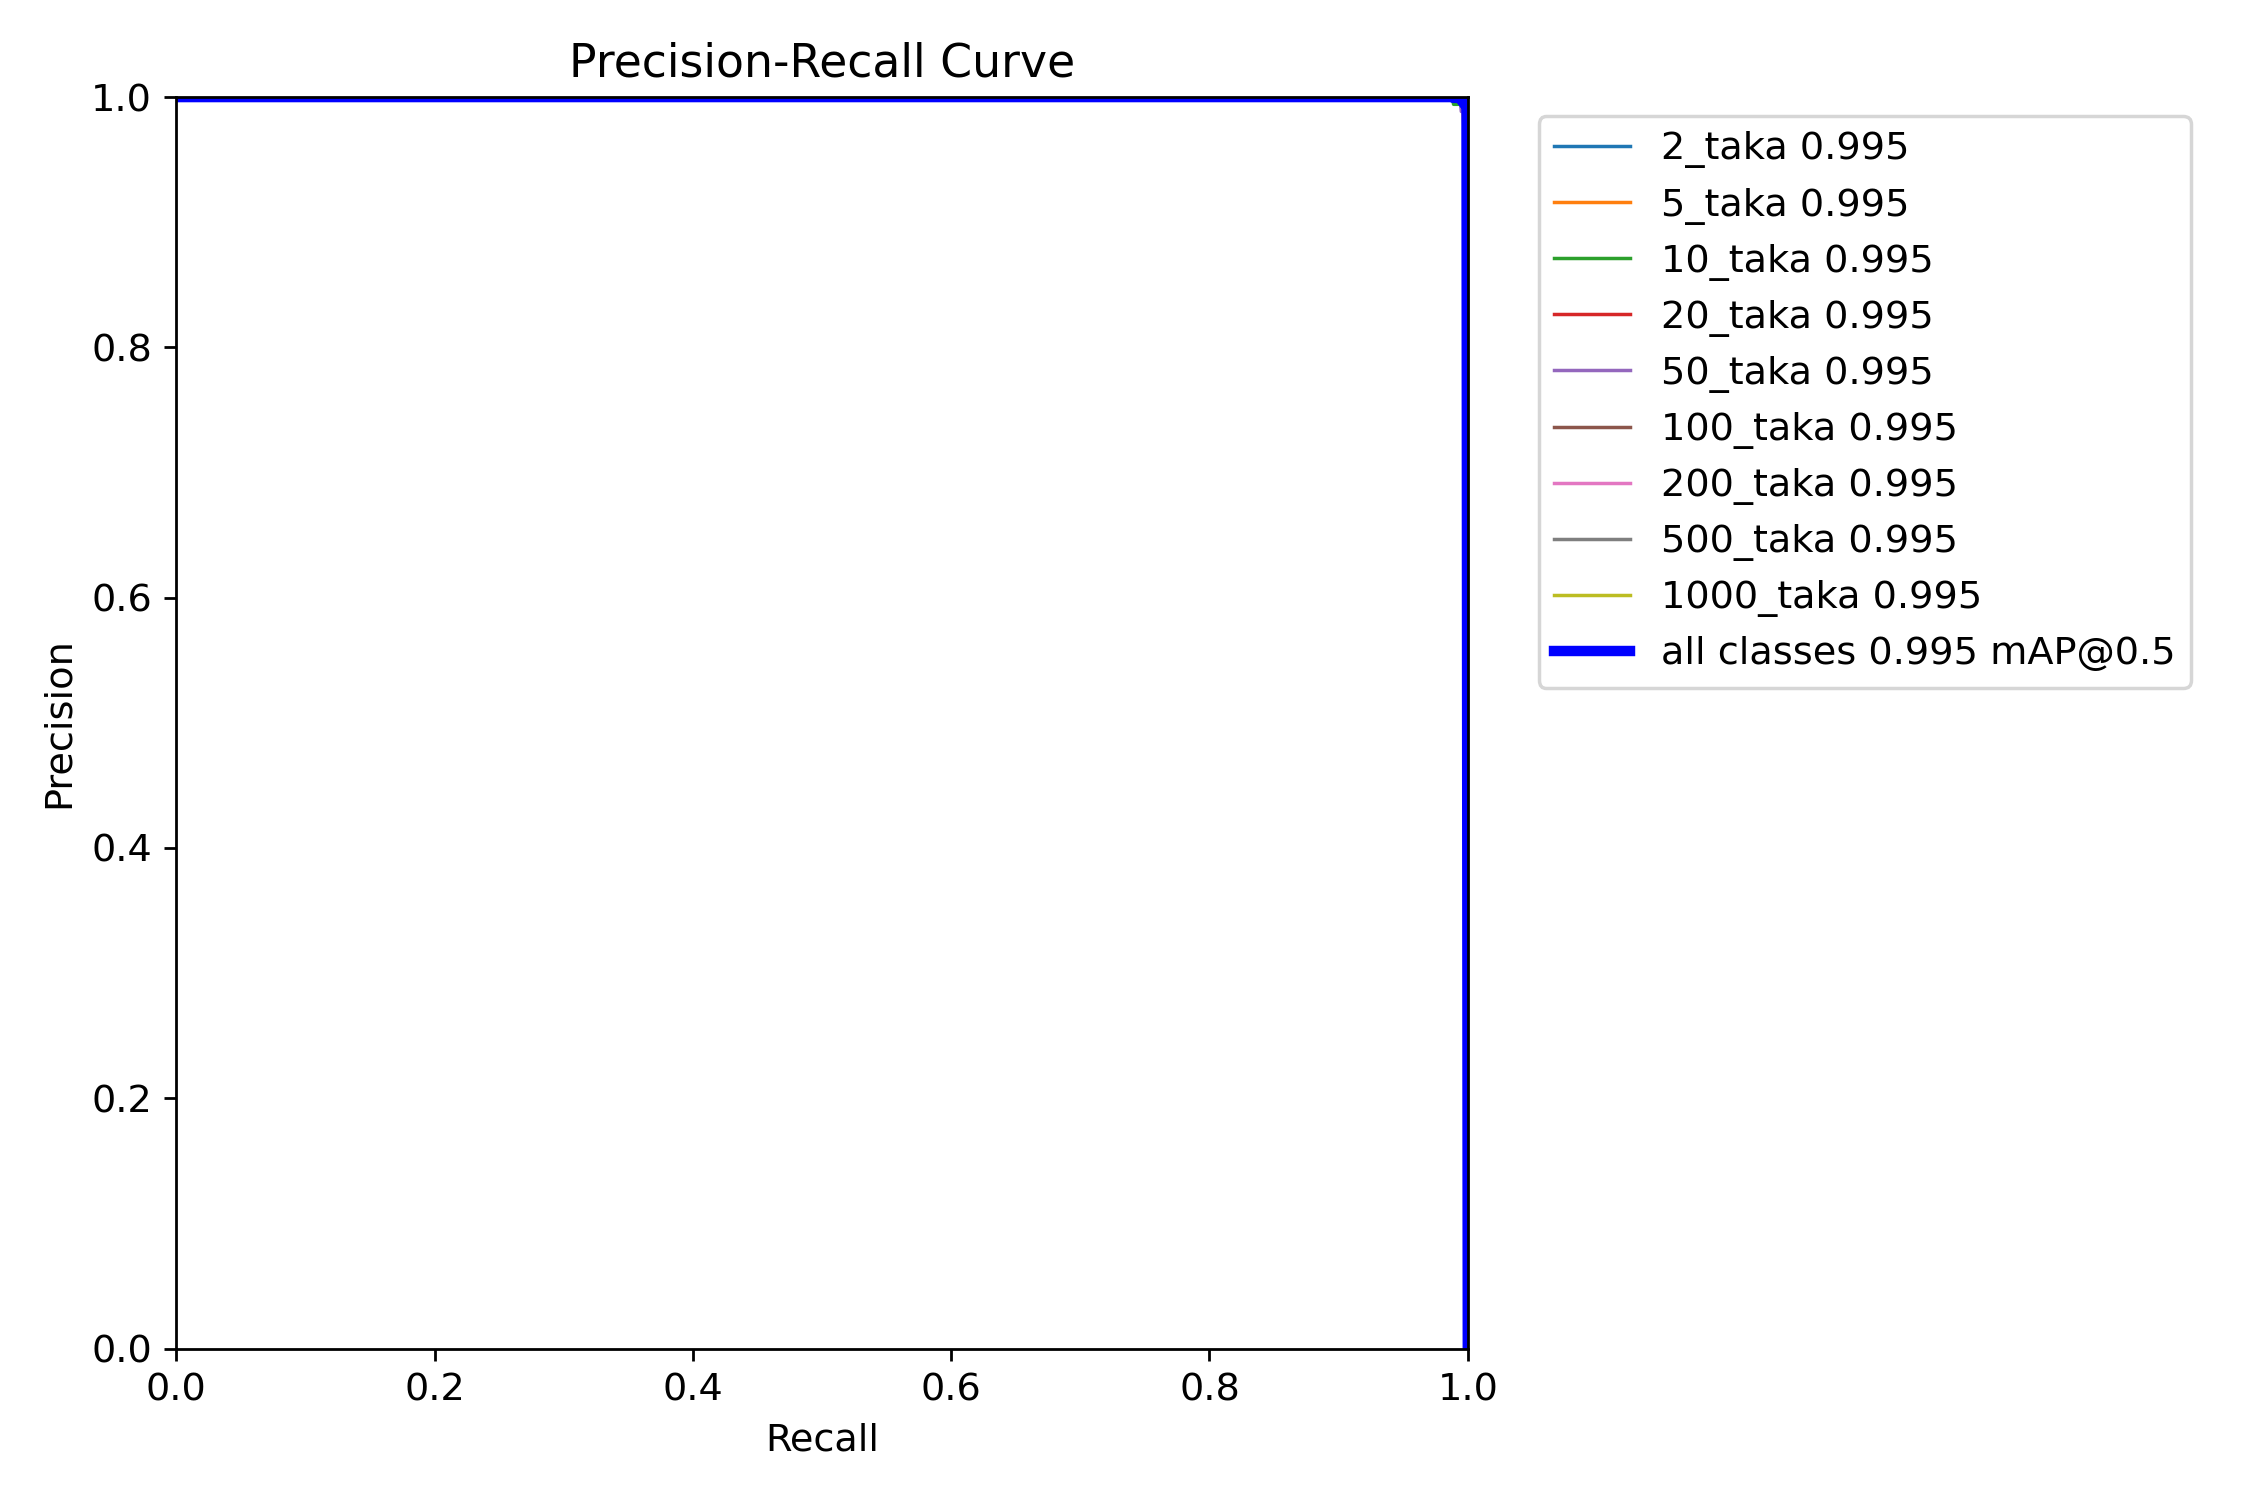
\includegraphics[width=0.75\textwidth]{fig_pr_curve.png}
  \caption{Precision--recall curves of the YOLOv8s Taka detector for all nine classes on the held-out synthetic test set}
  \label{fig:app_pr}
\end{figure}

\subsection{Sample Detections}
\begin{figure}[H]
  \centering
  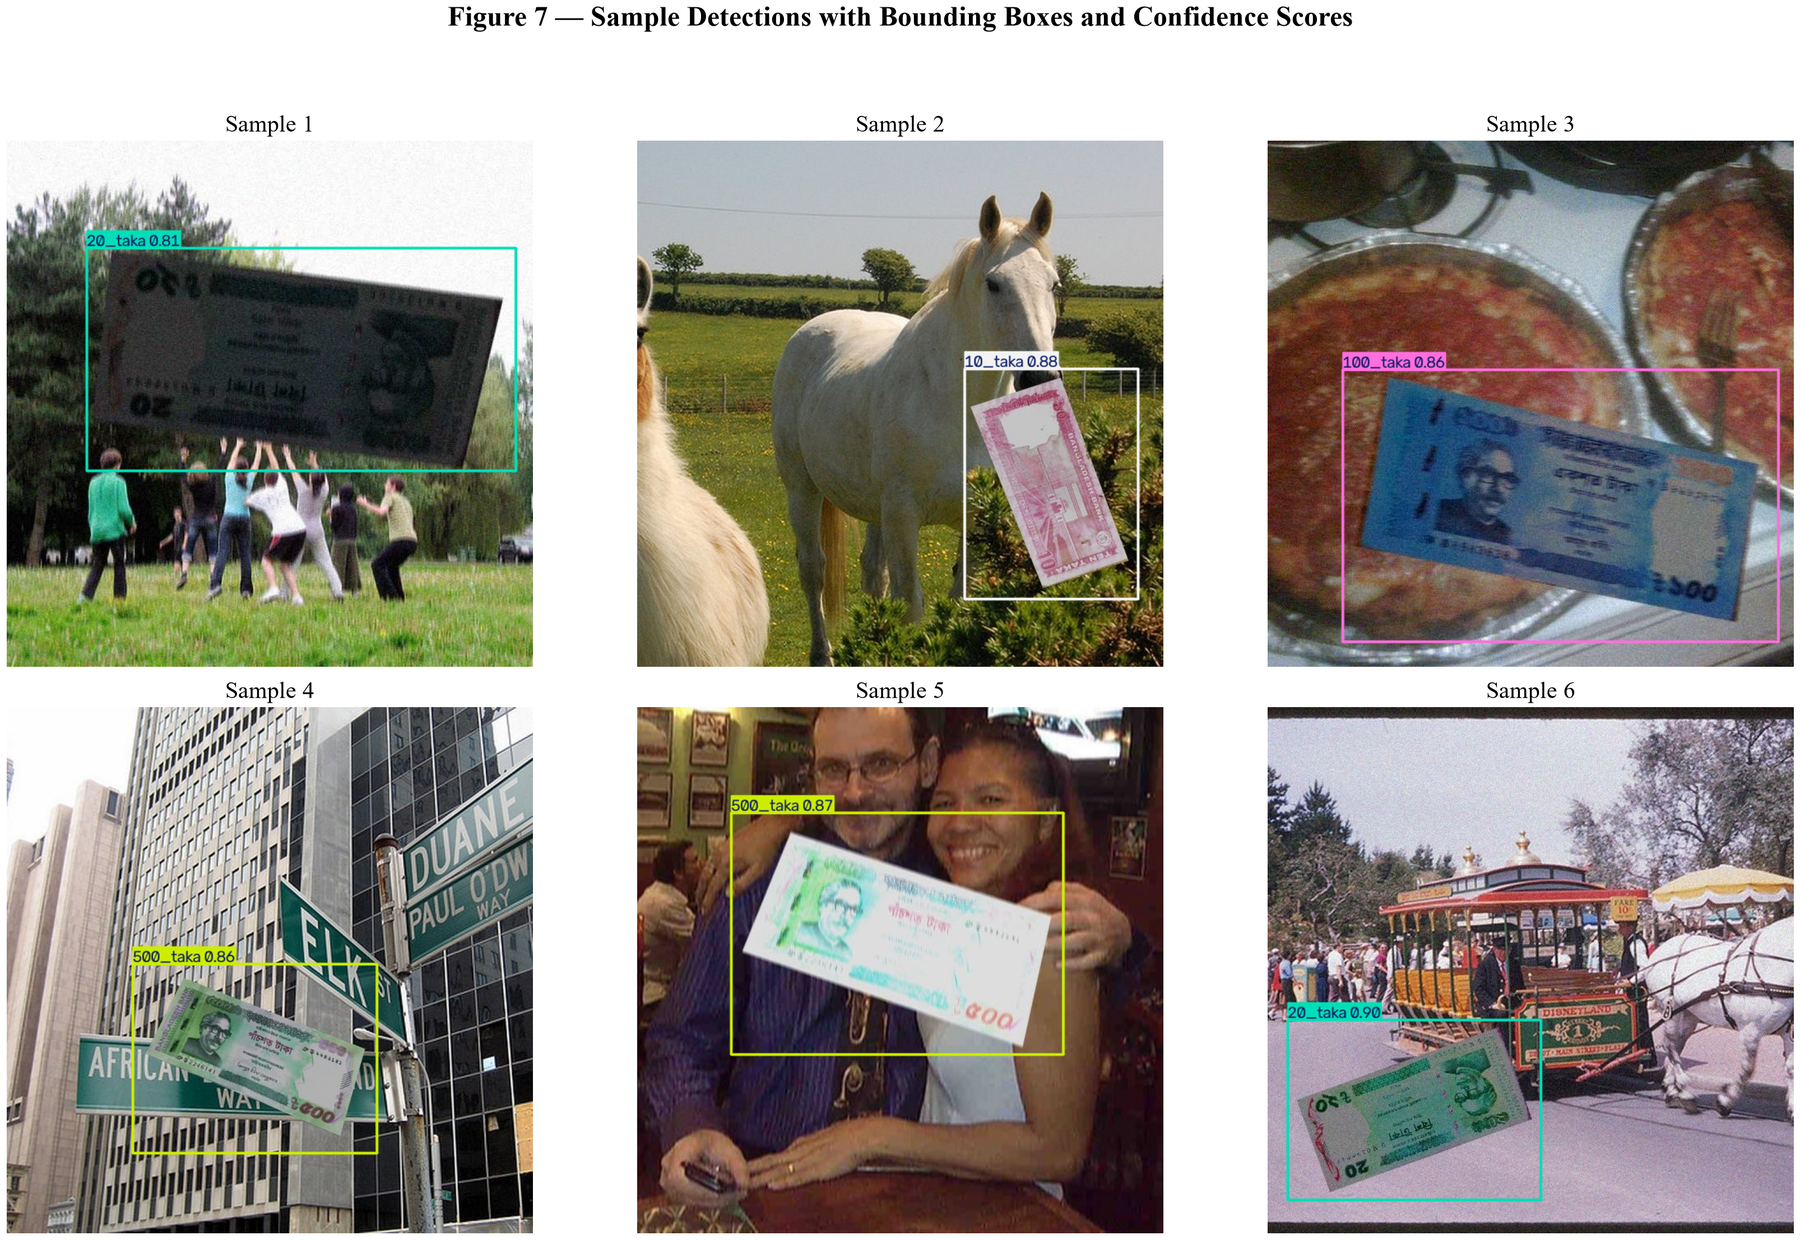
\includegraphics[width=\textwidth]{fig7_sample_detections.png}
  \caption{Sample detections of the Taka detector on composited scenes}
  \label{fig:app_samples}
\end{figure}

\subsection{Authentication Calibration}
\begin{figure}[H]
  \centering
  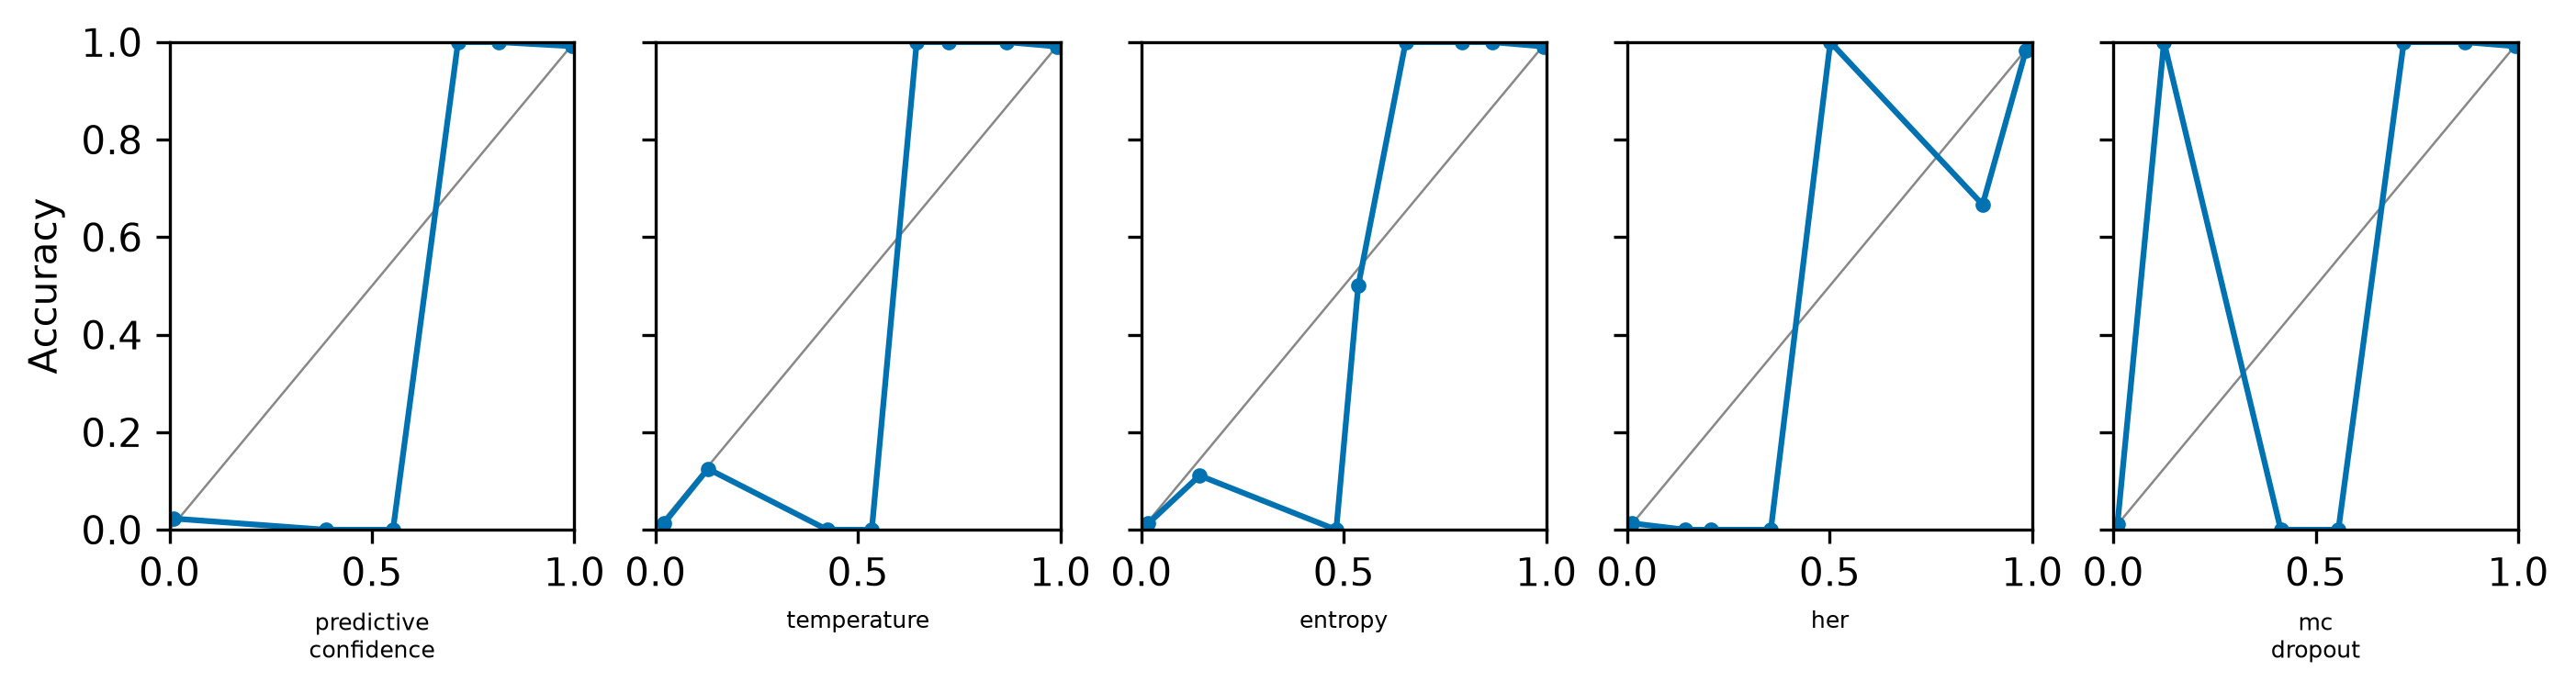
\includegraphics[width=\textwidth]{fig_auth_calibration.png}
  \caption{Reliability diagrams of the authenticator at six views for five confidence estimates (raw predictive confidence, temperature scaling, entropy mapping, HER and MC dropout); calibration maps fitted on the validation split and evaluated on the test split}
  \label{fig:app_calib}
\end{figure}

\subsection{Authentication over Seeds}
\begin{figure}[H]
  \centering
  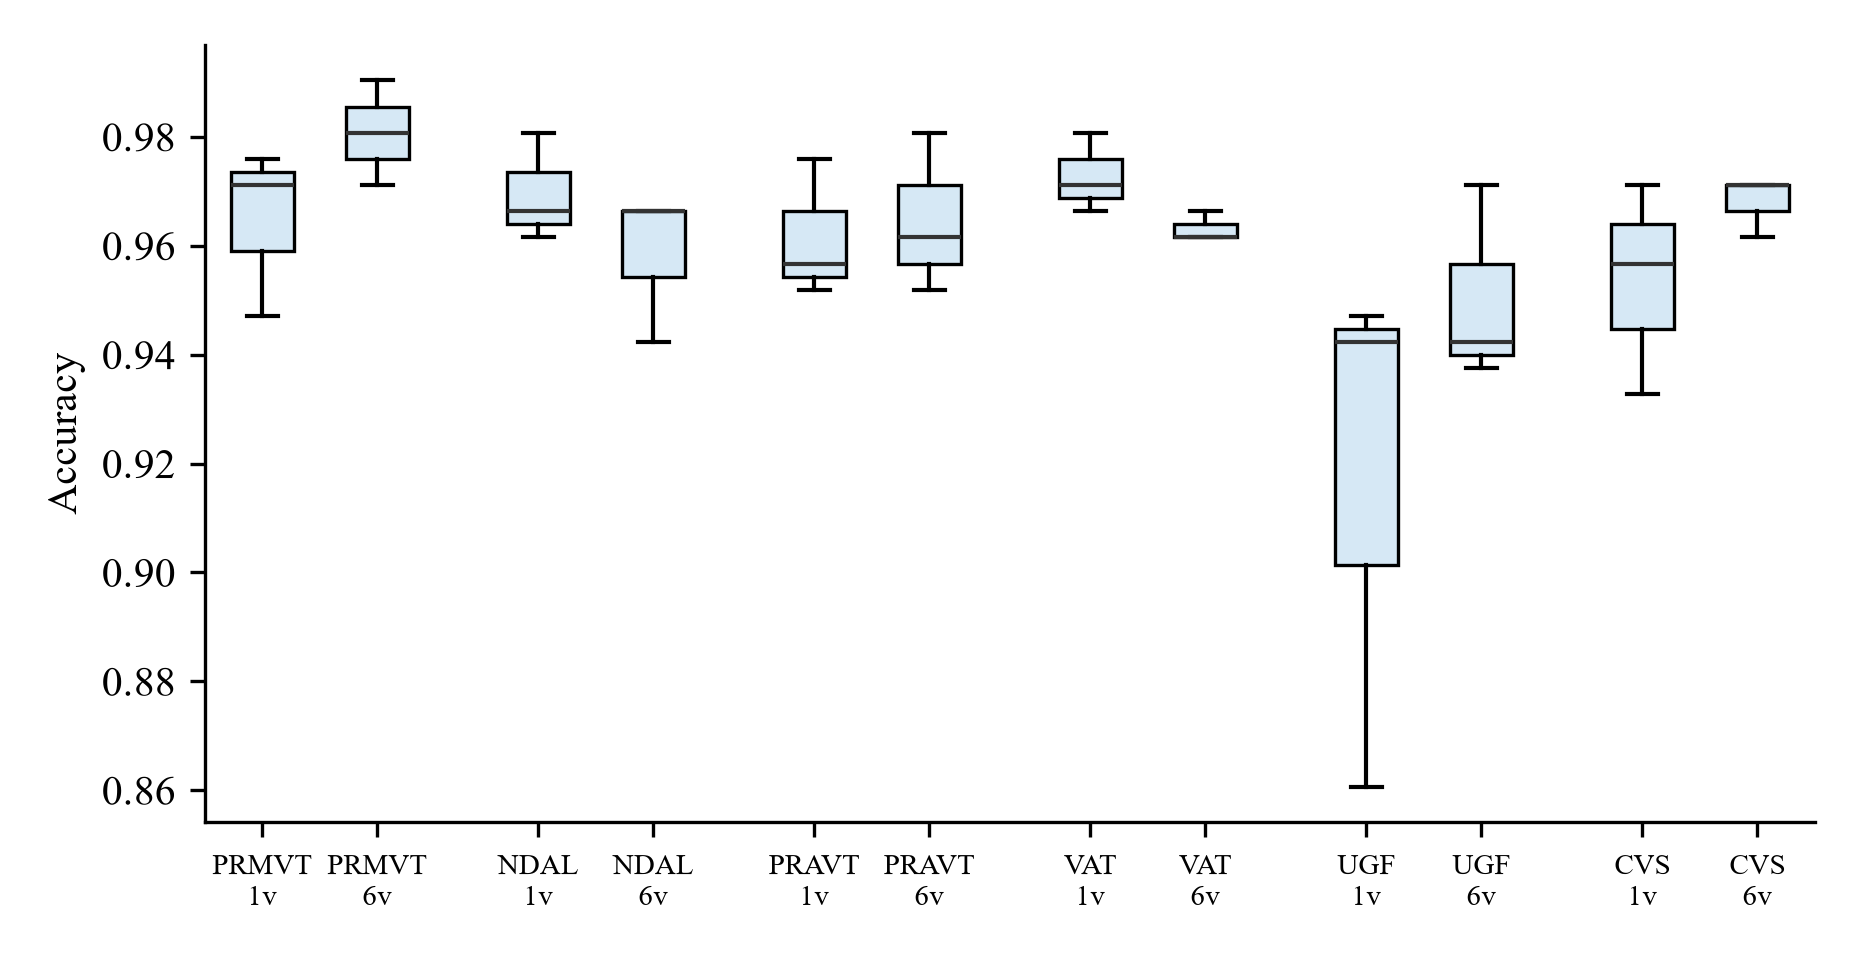
\includegraphics[width=0.8\textwidth]{fig_auth_multiseed.png}
  \caption{Spread of test accuracy over seeds 42, 43 and 44 at one view (1v) and six views (6v) for the main training variants}
  \label{fig:app_multiseed}
\end{figure}

\clearpage
\section{Configuration Parameters}
\label{app:config}

\begin{table}[H]
\centering
\caption{Main configuration parameters of Savior Glass (\texttt{config.py})}
\label{tab:app_config}
\small
\begin{tabular}{|l|c|p{4.8cm}|}
\hline
\textbf{Parameter} & \textbf{Value} & \textbf{Meaning} \\ \hline
OCR\_CONFIDENCE & 0.4 & Minimum EasyOCR confidence \\ \hline
OCR\_MIN\_CHARS & 3 & Shorter results are discarded \\ \hline
OBJECT\_CONFIDENCE & 0.50 & Minimum YOLO confidence for objects \\ \hline
CURRENCY\_CONFIDENCE & 0.65 & Minimum MobileNetV3 softmax score \\ \hline
OBJECT\_SCAN\_INTERVAL & 1.5 s & Time between automatic object scans \\ \hline
OBJECT\_ANNOUNCE\_COOLDOWN & 4.0 s & Per-class repetition cooldown \\ \hline
DEFAULT\_VOLUME & 80\% & Volume at start \\ \hline
VOLUME\_STEP & 10\% & Change per button press \\ \hline
TTS\_QUEUE\_MAXSIZE & 5 & Maximum queued messages \\ \hline
TTS\_INTER\_UTTERANCE\_PAUSE & 0.15 s & Pause between segments \\ \hline
ESPEAK\_SPEED / PITCH & 135 wpm / 45 & espeak-ng voice settings \\ \hline
Button debounce & 250 ms & Ignore repeated edges \\ \hline
Camera & 640$\times$480, 30 FPS & Capture resolution \\ \hline
\end{tabular}
\end{table}

\begin{table}[H]
\centering
\caption{Training hyper-parameters of the YOLOv8s Taka detector}
\label{tab:app_yolo}
\begin{tabular}{|l|p{8cm}|}
\hline
\textbf{Item} & \textbf{Value} \\ \hline
Model & YOLOv8s (11.1 M parameters, 28.5 GFLOPs), COCO-pretrained \\ \hline
Epochs / patience & 80 / 15 \\ \hline
Image size / batch & 640 / 16 \\ \hline
Optimiser & SGD, lr0 = 0.01, lrf = 0.01, momentum 0.937, weight decay 0.0005 \\ \hline
Warm-up & 3 epochs \\ \hline
Loss weights & box (CIoU) 7.5, class (BCE) 0.5, DFL 1.5 \\ \hline
Online augmentation & mosaic 1.0, mixup 0.15, HSV (0.02, 0.7, 0.4), degrees 20, shear 5, scale 0.5, translate 0.1 \\ \hline
Flips & Disabled (left--right and up--down) \\ \hline
Framework & Ultralytics 8.4.64, PyTorch 2.6.0 + CUDA 12.4 \\ \hline
\end{tabular}
\end{table}

\section{Reproducing the Results}
\label{app:repro}
\begin{lstlisting}
# Taka detector (Windows, from realtime_bangla_taka_detection/)
python -m venv venv
.\venv\Scripts\pip.exe install -r requirements.txt
.\venv\Scripts\python.exe scripts\download_backgrounds.py
.\venv\Scripts\python.exe scripts\generate_synthetic_dataset.py
.\venv\Scripts\python.exe scripts\train.py
.\venv\Scripts\python.exe scripts\evaluate.py
.\venv\Scripts\python.exe scripts\realtime_detect.py   # live demo

# Smart glass on Raspberry Pi 5 (from savior_glass/)
chmod +x install.sh && ./install.sh
sudo systemctl enable --now smart_glass.service

# Smart glass on Windows without GPIO
python test_windows.py
\end{lstlisting}


\phantomsection
\nocite{*}
\printbibliography[heading=bibintoc]

\end{document}
